%%==================================================
%% thesis.tex
%%==================================================

% 双面打印
\documentclass[master, adobefonts, openright, cs4size]{TJUgraduates} 
% \documentclass[bachelor, adobefonts, openright, cs4size]{TJUgraduates} 
% \documentclass[master]{TJUgraduates} 
% \documentclass[%
%   bachelor|master|doctor 
%   adobefonts, winfonts  	% 修改 /ctex 中的adobefonts, 改为mac默认中文字体
%   openany|openright 		% 单面打印,双面打印(默认)
%   cs4size|c5size 		% 正文字号:小四、五号(默认)
% ]

\usepackage{zhfontcfg}
\usepackage{siunitx}
\usepackage{booktabs}
\usepackage{textcomp}
\usepackage{paralist}

\begin{document}
\title{衰减介质的反射全波形反演方法研究}
\projectsource{}

\author{邹鹏}
\advisor{程玖兵 ~ 教授}
\defenddate{2018-06}
\school{同济大学}
\institute{海洋与地球科学学院}
\studentnumber{1533006}
\major{地球物理学}
\discipline{理学}
\faculty{海洋与地球科学学院}

\englishtitle{Reflection Full Waveform inversion in Attenuation Media}
\englishauthor{\textsc{Peng Zou}}
\englishadvisor{Prof. \textsc{ Jiubing Cheng}}
\englishschool{Tongji University}
\englishinstitute{\textsc{Depart of Geophysics, School of Ocean and Earth science} \\
  \textsc{ Tongji University} \\
  \textsc{Shanghai, P.R.China}}

\englishdiscipline{Natural Science}
\englishfaculty{Ocean and Earth Science}

\englishmajor{Geophysics}
\englishdate{May, 2017}

\resume{

\vspace{-5ex}
邹鹏,男,土家族,1993年03月出生于贵州思南。\\
2011年9月,考入同济大学海洋与地球科学学院。 \\
2015年6月,获地球物理理学学士学位。\\
2015年9月,免试直接攻读同济大学固体地球物理学硕士学位至今。
}


\include{frontmatter/cover}
%%==================================================
%% abstract.tex for TJU Master Thesis
%% based on CASthesis
%% version: 0.3a
%% Encoding: UTF-8
%% last update: Dec 5th, 2010
%%==================================================


%中文摘要

\begin{abstract}

实际地球介质是非弹性的,当地震波在地层中传播时将引起地震衰减,衰减强度通常
用品质因子$Q$来描述。强地震衰减往往出现在油气勘探的目标区域如汽云、
汽包区。地震衰减对地震波的运动学和动力学特征都会产生影响:速度频散和振幅衰减。
在地震数据处理中,如果不考虑地震衰减效应将直接影响储层识别和解释的可靠性。
在偏移成像中可以通过衰减补偿来校正速度频散和能量损失。然而所有的带
衰减补偿的偏移算法均需要相对准确的背景$Q$模型。

$Q$模型估计一直是地震学和勘探地震学领域的研究热点之一。早期用衰减前后地震波
的振幅谱的比值来构建层析矩阵,为了消除非衰减因素对振幅谱的影响,学者们通过检测
质心频率的变化来反演$Q$值。这类方法通过射线追踪计算层析矩阵,当介质变化复杂时
射线理论由于存在焦散以及多路径效应,从而降低了此类方法反演的精度。
随着高性能计算机技术的不断进步以及宽频带、宽方位、高密度地震数据采集技术的逐渐
成熟,单参数速度的全波形反演(FWI)技术逐渐走向成熟。近年来,粘声介质的全波形
反演($Q$-FWI)技术也得到了飞速发展。$Q$-FWI以波动方程为传播引擎,能适应复杂地质
情况,但其利用的主要是透射波信息,透射波对地下的穿透深度有限。当缺乏低频、长
偏移距数据时,$Q$-FWI只能反演得到浅层的模型参数。为了获得中深部的$Q$模型,
在成像域中提出了偏移$Q$分析方法。但成像域方法相较于数据域方法其分辨率偏低。

本文第3章首次将$Q$反演纳入反射全波形反演($Q$-RWI)框架。当观测地震数据缺少大孔径的
折射波信息时,$Q$-RWI利用反射波数据更新中深层模型。$Q$-RWI强烈依赖高波数速度
模型,在缺乏$Q$信息的情况下,最小平方逆时偏移(LSRTM)没法给出准确的高波数
速度模型。为了降低$Q$-RWI对速度模型高波数成分的依赖性,论文第4章引入了峰值频率
移动目标函数来更新中深层$Q$模型。峰值频率是地震数据的一个属性,其大小只与地震子波
以及地层的衰减有关,只要速度的高频成分不影响地震子波的形状即不会改变峰值频率的大小。
在实际反演中用层状速度平滑差代替高波数速度扰动即可满足要求。

本文针对中深层背景$Q$反演遇到的问题,提出了$Q$-RWI反演方法。通过峰值频率移动
目标函数的引入全完降低了$Q$-RWI对高波数速度模型的依赖,使$Q$-RWI方法更加
实用化。




  \keywords{\zihao{-4} 
  	地震衰减,  
  	全波形反演, 
  	粘声反射全波形反演,  
  	峰值频率,  
  	衰减补偿逆时偏移 
  	}
\end{abstract}



%英文摘要


\begin{englishabstract}






  \englishkeywords{\zihao{-4}  
  	test, 
  	test, 
  	test,
  }
  
  
\end{englishabstract}
 %% 摘要
%% 目录、插图目录、表格目录
\tableofcontents

\listoffigures
\addcontentsline{toc}{chapter}{\listfigurename} %将插图目录加入全文目录

%\listoftables
%\addcontentsline{toc}{chapter}{\listtablename}  %将表格目录加入全文目录

		%%==================================================
%% symbol.tex for SJTU Master Thesis
%% based on CASthesis
%% modified by wei.jianwen@gmail.com
%% version: 0.3a
%% Encoding: UTF-8
%% last update: Dec 5th, 2010
%%==================================================

%\chapter{主要符号对照表}
%\label{chap:symb}
%
%
%\begin{center}
%	
%
%\vspace{1cm}
%\begin{tabular}{ll}
%	$\alpha$ \qquad & \hspace{5em}test \\
%
%\end{tabular}
%
%
%\end{center}
 % 主要符号、缩略词对照表



\mainmatter	% 使用阿拉伯数字对正文编号

%% 正文内容
%%==========================
%% chapter01.tex for TJU Master Thesis
%% based on CASthesis
%% modified by charlie.yaha@gmail.com
%% version: 0.1alpha
%% Encoding: UTF-8
%% last update: Dec 5th, 2010
%%==================================================

%\bibliographystyle{TJU} %[此处用于每章都生产参考文献]


\newcommand{\citeA}[2]{\citeauthor{#1}\cite{#1}}

\chapter{绪~论}

\section{研究背景及意义}
地下介质普遍具有非弹性衰减性质,其衰减性通常用品质因子$Q$来表征。
地震尺度内的非弹性衰减主要是与介质内部介关尺度(介于波长与颗粒尺度之间)的
弹性非均匀性或流体饱和非均匀性诱导的波致流体流现象有关
(\citeA{pride:2003},\citeA{muller:2010})。
地震波衰减对地表观测数据有非常重要的影响,
主要表现在如下两方面:首先,衰减会减弱地震波的振幅;其次,衰减改造地震波相位以致
速度频散。图(\ref{fig:spectral}a)对比了在同一时刻接收的
非衰减介质中的地震波(蓝色)和在$Q=60$的粘声介质中传播的地震波的波形。可以看出,衰减介质中传播地震波
的振幅被极大程度地吸收衰减。由于地震波衰减导致速度频散,高频成分具有更快的传播速度,所以
不同频率成分具有不同的到达时。
图(\ref{fig:spectral}b)对应地展示了图(\ref{fig:spectral}a)中两种波形的振幅谱。
从图中可以看出,高频成分的衰减要
远远严重于低频成分,这也是造成图(\ref{fig:spectral}a)中振幅强衰减的主要原因。

\begin{figure*}[!htbp]
        \centering
		\subfigure[]{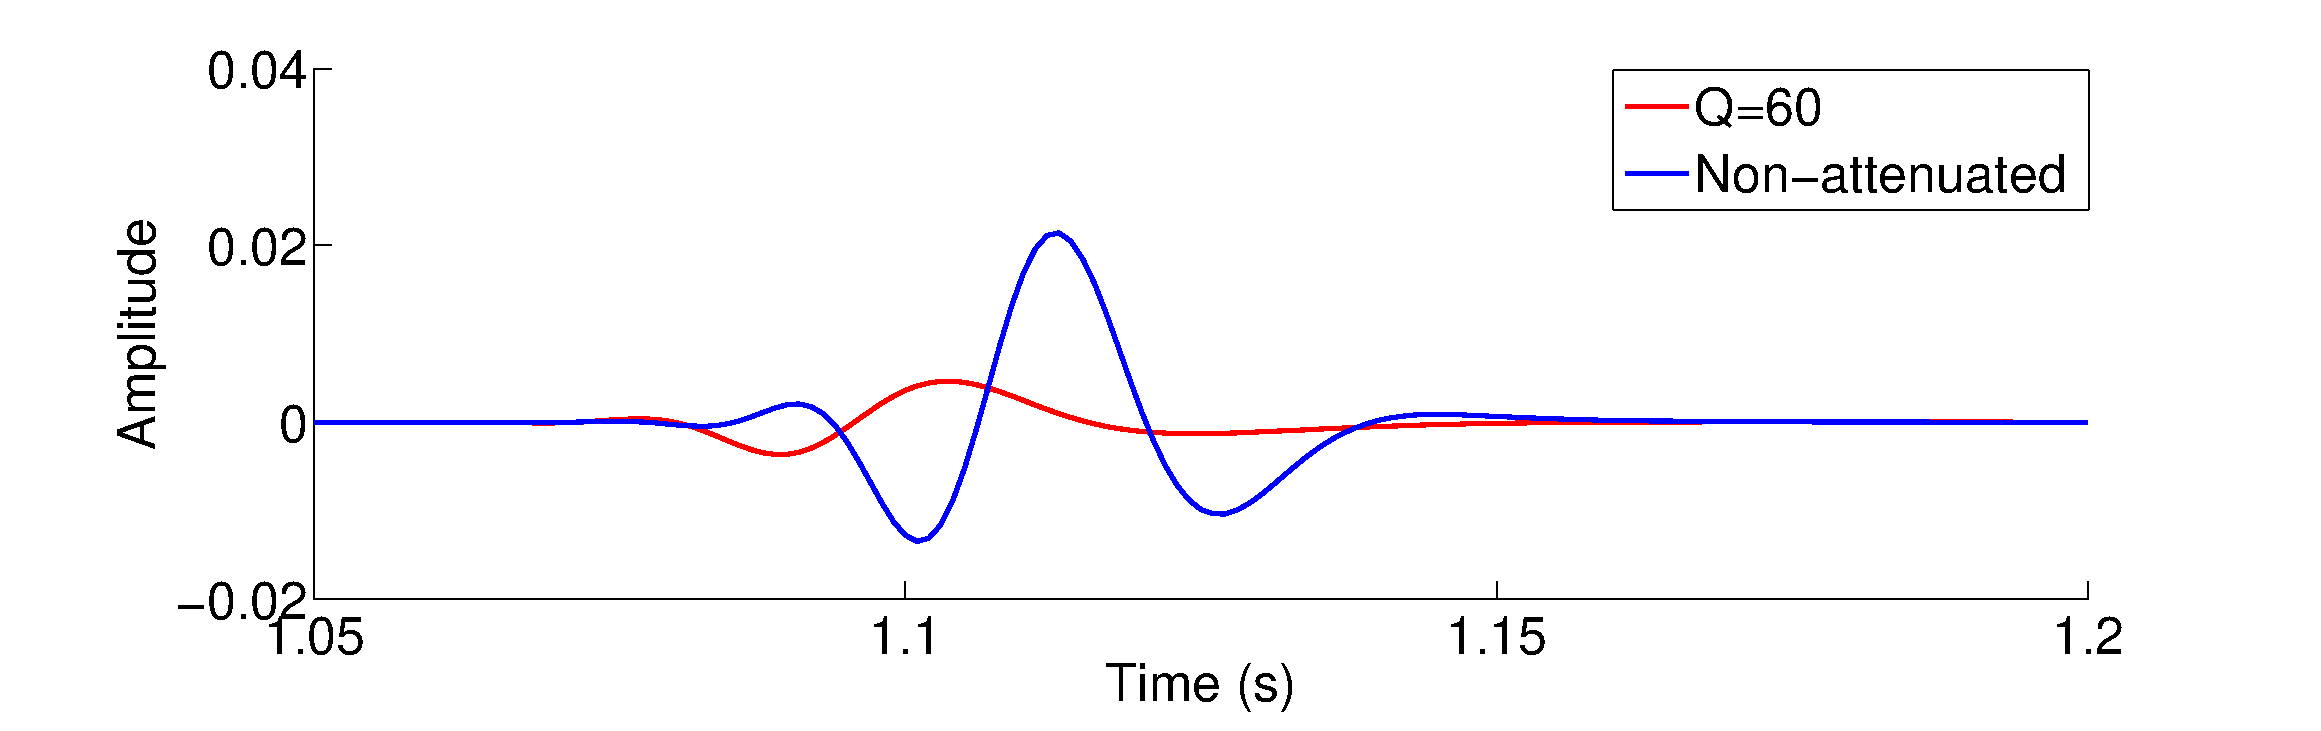
\includegraphics[width=0.9\linewidth]{figure/wavelet_ch1}}
		\subfigure[]{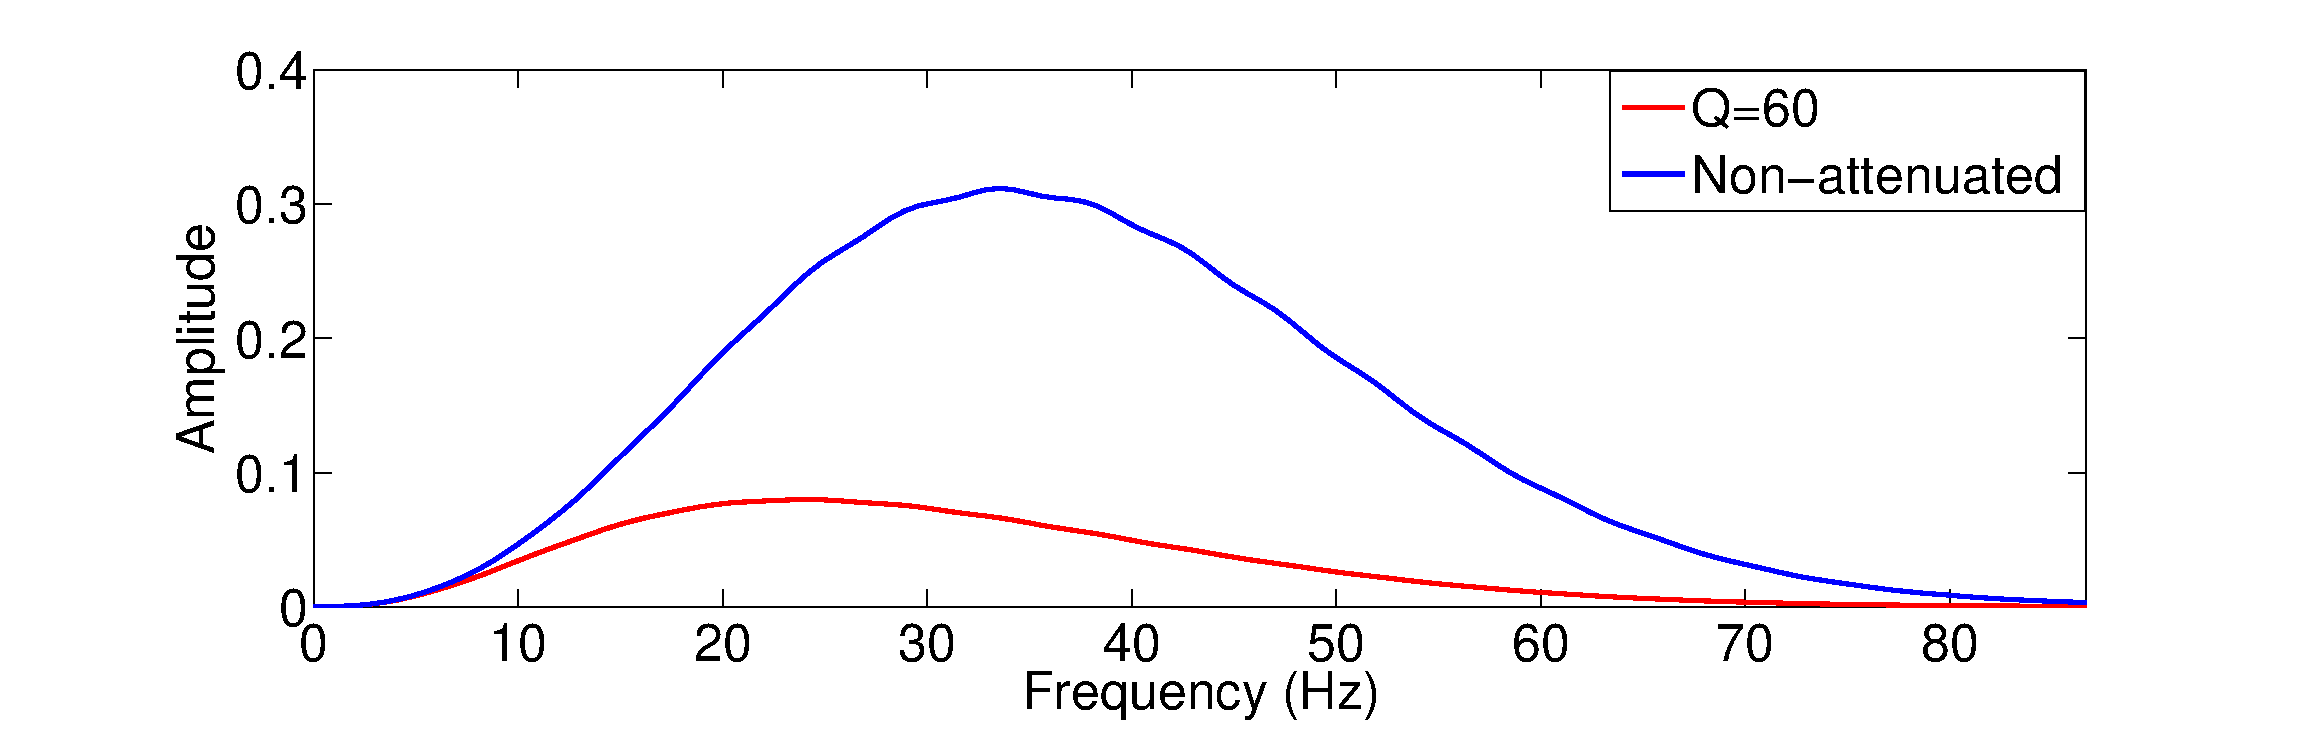
\includegraphics[width=0.9\linewidth]{figure/spectrum_ch1}}
        \fcaption{地震波在声介质和粘声介质($Q=60$)中传播的数值模拟实验:
	(a)地震波波形图;(b)对应的振幅谱。}{1D example to numerically illustrate the attenuation 
	impacts on the amplitudes spectra and phase of propagating wave: (a) the 
	non-attenuated waveform (blue curve) and the attenuated waveform (red curve); (b) the 
	corresponding amplitude spectral. }[展示地震衰减效应的一维数值实验]
        \label{fig:spectral}
\end{figure*}

非弹性衰减通过吸收地震波的
高频成分和改造地震波的相位来降低地震波成像的分辨率。在地震波偏移成像中,
如果不补偿$Q$的效应会影响地震成像的质量进而影响后续的地震解释和储层识别。
图(\ref{fig:qrtm_1}a)展示了墨西哥湾某工区常规
逆时偏移(RTM)成像结果,图(\ref{fig:qrtm_1}b)对应地展示了用$Q$补偿的逆时偏移($Q$-RTM)
成像结果(\citeA{zhang.zhang:2010})。由于强衰减的影响,使得常规RTM在衰减区域及其下方成像模糊,
通过$Q$补偿使得整个成像剖面的振幅更加均衡,且很好地恢复了由衰减引起的成像阴影区的地层信息。

\begin{figure*}[!htbp]
        \centering
		\subfigure[]{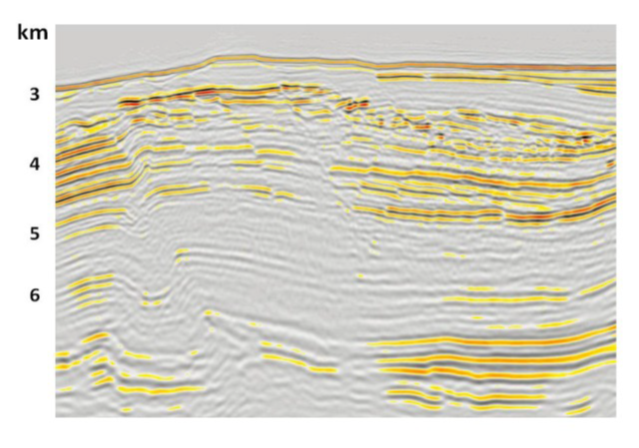
\includegraphics[width=0.495\linewidth]{figure/mig_no_ch1}}
		\subfigure[]{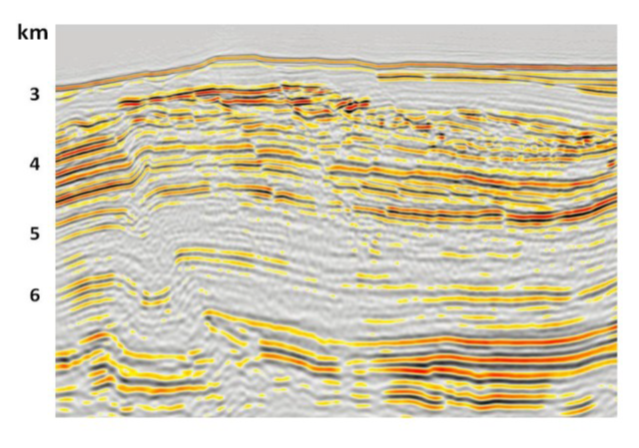
\includegraphics[width=0.495\linewidth]{figure/mig_q_ch1}}
		\fcaption{衰减对地震成像的影响:(a) 传统RTM成像结果;(b)$Q$-RTM成像结果
		(\citeA{zhang.zhang:2010})。
		}{A comparison of conventional RTM (a) and $Q$-RTM (b) results..
		}[衰减对地震成像的影响]
        \label{fig:qrtm_1}
\end{figure*}

在实际勘探中,气云区的地震成像、解释和储层识别都面临巨大的挑战。气云区通常包含极低的
$Q$值,强烈的衰减会吸收深部反射波的能量,在储层的上方造成成像阴影区,严重影响地震
解释的准确性。可靠的$Q$模型不仅可以提高成像的质量,而且可以更好解释振幅随偏移距变化
(AVO)和各向异性这两种依赖于偏移距的效应。正确的AVO和各向异性
解释可以提高油气勘探的成功率。另外,$Q$模型可以作为一个表征岩石和流体属性的参数。
例如,在稀疏井约束下可以用$Q$值来检测岩性的边界(\citeA{desgupta.clark:1998})。
衰减系数是一个直接刻画储层的油气物理参数,例如可以利用$Q$模型来确定储层含油/气
的饱和度(\citeA{winkler.nur:1982})。在油气开发过程中,衰减模型还可以用来指示储层裂缝的方位
(\citeA{maultzsch.chapman:2007}; \citeA{clark.benson:2009}),也可监控流体的运移能力,
帮助优化注水过程(\citeA{macrides.kanasewich:1987})。
因此,在油气勘探开发过程中,定量地评估非弹性衰减效应,构建一个可靠的本征衰减($Q$)模型是非常重要的。
鉴于地震波非弹性衰减的路径效应比界面影响更大,
本文主要的工作就是通过反射波形反演来定量估计宏观的地震本征衰减$Q$模型。

\vspace{1.0cm}
\section{国内外研究现状}

国内外学者对$Q$模型估计开展了大量的研究,其中大部分工作都是数据域的分析和反演方法。数据域的
$Q$反演方法可大致分为两类:基于高频近似的射线层析类和基于波动方程的波形反演类。

在射线类层析方法中,\citeB{brzostowski.mcmechan:1992}首先用观测数据振幅与震源振幅比值的对数作为输入数据来
实现$Q$层析成像。除了吸收衰减外,影响振幅的因素还有很多,如几何扩散、透射/反射损失、
散射损失等。为了区分衰减引起的振幅损失,\citeB{quan.harris:1997}将观测数据和计算数据之间质心
频率的移动作为匹配依据,用射线层析来更新$Q$模型。\citeB{hu.liu:2011}用震源的振幅谱作为
拟合函数来处理地震数据频谱非对称性的影响,并用多指数盒状约束法来消除非地震本征衰减的影响。
质心频率移动类的方法相对于振幅匹配类方法对噪音不敏感,更适合处理实际地震数据。
射线类方法计算效率高,处理横向变化缓慢的介质有很好的效果。当上覆介质横向非均匀性很强时,
地震波存在多路径,射线类方法由于不能有效处理多路径效应而造成误差。波动方程层析方法可以
有效的解决多路径问题,从而提高反演的分辨率。

全波形反演(FWI)是一种通过求解波动方程来恢复地下介质参数的反演迭代方法(\citeA{tarantola:1984})。
FWI是一个高度非线性的反演问题(\citeA{mora:1987};\citeA{sirgue.pratt:2004}),需要
大量的波场正演计算,全局寻优的解法(\citeA{sen.stoffa:1991};\citeA{mosegaard.tarantola:1995})
所需的计算量仍是现在计算机所不能承受的。伴随状态法的引入(\citeA{lailly:1983};
\citeA{tarantola:1984};\citeA{pratt.worthington:1990})使得目标函数梯度的计算变得非常高效,目前基于
梯度类的解法已趋于成熟。在勘探地震学中,各种应用实例证明粘声波形反演($Q$-FWI)对于提供高
分辨率的P波速度结构有非常重要的作用(\citeA{song:1995};\citeA{ravaut:2004} 
;\citeA{gao:2006}; \citeA{kamei:2012})。由于衰减参数相较于速度参数对目标函数
的影响更弱且这两种参数之间还存在强烈的耦合性(trade off),衰减参数的波形反演比速度的波形反演更具挑战性(
\citeA{song:1995};\citeA{liao.mcmechan:1996};\citeA{smithyman:2009};\citeA{hak.mulder:2011} 
;\citeA{malinowski:2011};\citeA{bai:2014};\citeA{kamei.pratt:2013})。

\citeB{tarantola:1988}在时间域粘弹波形反演理论中首次考虑了衰减参数的波形反演。
随后,\citeB{song:1995}在频率域提出了一种粘声波形反演方法。在频率域实现波形反演比时间域
有如下优势,尤其是考虑衰减效应: 首先,衰减参数(例如$Q$值)和频散速度关系很容易用随频率
变化的复速度来表示,目标函数对速度和衰减参数的梯度可以同时得到而不需要额外的计算量(\citeA{song:1995})。
另外,频率域反演方法可以自然的实现多尺度反演策略以降低波形反演的非线性(\citeA{bunks:1995};
\citeA{sirgue.pratt:2004})。从最低的频率成分开始反演,并逐渐增加高频成分,这样可以
逐渐重建高分辨率的地下速度和衰减模型。

在波形反演中,速度和衰减参数$Q$有很强的耦合性(\citeA{song:1995};\citeA{kamei.pratt:2008};
\citeA{hak.mulder:2011})。\citeB{ribodetti:2000}以及\citeB{hak.mulder:2010}讨论了观测系统的
重要性。他们指出,完美的地下照明可以解决这种参数串扰问题。\citeB{innanen.weglein:2007}用逆散射
理论和一阶的频散反射系数来区分一维速度和衰减系数结构。\citeB{mulder.hak:2009}调查了
线性Born反演的零空间情况,并且指出,在计算梯度时如果不考虑速度频散关系,对于给定的地表反射数据,
地下许多速度/衰减对存在无解的情况。\citeB{hak.mulder:2011}指出,对于地表观测系统,考虑了频散关系
的非线性波形反演可以较精确地反演简单二维理论模型的速度和衰减系数。
然而,在早些阶段的反演中,串扰现象还是很明显,并且需要非常多(在他们的实验中大于10000次)的迭代
次数来消除,因此该反演问题还是非常病态的。此外,由于参数间强耦合性的影响,
考虑纵横波速度、密度、衰减参数的弹性波形反演
(\citeA{yang:2017},\citeA{fabien:2017})更有挑战。

在$Q$-FWI中,各种各样的预条件方法被用来减弱反演的病态性。\citeB{liao.mcmechan:1996}用合成数据
实验显示要获得好的衰减模型,必须要对模型参数进行一定的范围约束。\citeB{hak.mulder:2011}指出
基于两种参数特征值的大小来惩罚梯度中衰减成分可以加速$Q$-FWI的收敛。\citeB{malinowski:2011}
在波兰某盆地成功地反演出了与岩性信息一致的衰减模型。他们指出对地震数据时间方向强阻尼衰减
和梯度大尺度平滑约束是反演$Q$参数的关键。

对于$Q$反演的另一类做法是顺序反演,即先获取比较准确的速度模型然后再反演$Q$模型。如果我们认为
反演前期的振幅变化主要是由于速度结构引起的,后续再反演$Q$时可以降低参数间的串扰。初始的速度估计是通过
固定初始衰减模型来反演(\citeA{pratt:2004};\citeA{kamei.pratt:2008};\citeA{rao.wang:2008};
\citeA{smithyman:2009})。\citeB{pratt:2004}用顺序反演法处理含碳氢化合物的强衰减跨井数据。
对于$Q$模型的反演,他们也用了较大的平滑约束,其反演结果与超声波形分析结果有很好的一致性。
\citeB{watanabe:2004}在超声频段用实验室数据同样很好实现了顺序反演方法。\citeB{smithyman:2009}
用顺序反演法来识别近地表非弹性衰减目标体。\citeB{watanabe:2004}以及\citeB{kamei.pratt:2008}用合成跨井数据
比对了同时反演和顺序反演的结果,发现在没有正则化项约束的情况下,顺序反演会得到更好的结果,
他们认为地震数据中大部分振幅变化是由速度变化引起的。
\citeB{kamei.pratt:2013}系统地调查了不同梯度预条件对$Q$反演的影响。

地震数据的走时信息主要受速度参数影响,地震衰减通过速度频散影响走时,但衰减的振幅效应
更明显。相较于走时信息,地震振幅很容易受噪音、震源检波器的耦合、震源的辐射模式以及
弹性(非声学)效应的影响。为了保证振幅信息的准确性,需要非常细心的前处理工作(\citeA{pratt:2004};
\citeA{malinowski:2011})。\citeB{dutta.schuster:2016}通过将峰值频率移动引入到$Q$-FWI中
来降低数据对前处理的依赖,从目标函数出发降低了$Q$-FWI的非线性程度。

FWI需要低频、全方位、大孔徑地震数据,但是这种高质量的数据采集往往需要高昂的代价。
通过不同观测孔径的观测系统照明分析可知,当缺少大孔径的回转波或折射波数据时,深部模型往往只被
反射波照明。因此,利用反射波进行中深部的速度建模已成为共识。
当反射数据占主导时,常规FWI的梯度中高频成分占主导,反射波的偏移响应与利用反射波反演
背景模型的核函数相比,数值上往往高一个数量级,因此,常规FWI只会得到一个
高波数的成像结果,不易于更新背景模型(\citeA{wu.alkhalifah:2014};\citeA{alkhalifah:2015};
\citeA{chi:2015};\citeA{alkhalifah.wu:2016})。
为改善对模型低频成分的更新,学者们提出了梯度预条件方法(\citeA{Liu:2011};\citeA{wang:2013};
\citeA{tang:2013}),目的是增强层析分量的贡献进而得到有效的低波数模型的更新。
为了解决反射波数据占主导情况下FWI的上述问题,\citeB{xu:2012a}提出了反射波形反演
方法(RWI)。其思想在于:将速度模型分解为背景模型和扰动模型两部分,利用反射波数据侧重更新
背景速度而非高波数的速度扰动。

但是,为了使RWI能够在实际地震资料反演中更好地恢复中深层背景速度,需要进行数据匹配和反射系数估计
(真振幅成像)。\citeB{ma.hale:2013}利用DIW算法(Dynamic image warping)提取反射波的走时时差,
实现中深层背景速度建模,提高反演的稳定性。\citeB{alkhalifah:2016}用散射角滤波的全模型反演方法
来解决数据分级匹配问题。基于相关的反射波形反演方法(\citeA{chi:2015}),在一定程度上也避免了
数据匹配的周期跳跃问题。即使在观测数据中缺乏有效低频信息、背景模型相对较差时,RWI也可以较好地
恢复模型中深部的低波数成分。在反射系数估计方面,最小二乘偏移(\citeA{dai.schuster:2013};
\citeA{zhang:2014})是目前比较有效的方法。但是,最小二乘偏移要求背景模型要足够准确
(\citeA{luo.hale:2014}),否则其反演的高波数模型扰动也不正确,而这又与
RWI反演背景速度的目标相矛盾。因此,在反射波波形反演中,如何以及何时引入最小二乘偏移将显得非常重要。
最近,\citeB{cheng:2018}提出了基于模型尺度分解,P/S波模式解耦的反射走时与波形反演方法,
交替更新纵横波速度的宏观背景与高波数扰动。这项工作对基于反射波的多参数反演有一定的借鉴意义。

此外,\citeB{shen.biondi:2018}在成像域建立起了模型扰动与偏移图像扰动的关系,
通过$Q$偏移分析估计中深层的背景$Q$模型。
目前还没人探讨用地表反射地震数据恢复中深层背景$Q$模型的数据域反演方法。
本文将研究如何把RWI引入到背景$Q$反演中。

\vspace{1.0cm}
\section{本文研究内容}

本征衰减参数$Q$对地震波振幅的影响类似于速度对走时信息的影响,是一种沿地震波路径累积叠加的效应,
并且主要受$Q$模型的低波数(背景)成分控制。在实际应用中,相对准确的背景$Q$模型即可补偿成像中
能量的损失和相位畸变,提高成像分辨率。本文结合地震衰减的具体特点,在RWI的框架下
,实现中深层背景衰减模型的反演。具体研究内容包括:

在第二章中,首先简单回顾了地震衰减的基本理论,分析表征地震衰减的物理参数(品质因子和吸收系数);
其次总结了描述地震衰减的本构关系,并重点回顾了勘探地震学中常用的两类衰减模型(标准线性固体模型
和常$Q$模型);然后推导了描述这两类衰减模型的粘声波方程,并比较了这两种方程波场模拟的结果;最后
总结了$Q$-RTM所遇到的问题及其解决办法,并比较了上述两类方程在$Q$偏移
成像中的应用。

在第三章中,在顺序反演的思路下,提出了宏观衰减模型反射波形反演($Q$-RWI)方法。
先假定速度模型准确,将速度分解为背景和扰动两部分,基于标准线性固体模型粘声波方程
通过Born正演实现反射波模拟。在RWI的框架下,用波形数据残差作为
目标函数来更新中深层背景$Q$模型。

在第四章中,首先讨论了反射地震数据的峰值频率属性与速度高波数模型的关系;其次用峰值频率
移动目标函数来降低$Q$-RWI对高波数速度模型的依赖;然后用短时傅里叶变换(STFT)
提取多反射震相数据的峰值频率;最后通过数值实验验证峰值频率移动目标函数
的可靠性。


最后,总结论文的主要结论和创新点,并讨论不足之处以及未来的研究方向。


















%%==================================================
%% chapter02.tex for TJU Master Thesis
%% based on CASthesis
%% modified by wei.jianwen@gmail.com
%% Encoding: UTF-8
%%==================================================

\chapter{衰减介质理论基础}

线性粘弹理论已趋于完善,\citeA{carcione:2007} 对其做了较为完整的总结。粘弹性介质的性质介于弹性固体与粘性流体之间,
可以定义为材料在一定的外力作用历史条件及其处于某一温度范围情况下所表现出来的同时具有弹性固体和粘性流体效应的性质。
除了当时所受外力大小外,外力加载时间、加载历史以及介质温度变化都会对粘性介质的形变产生影响。粘弹性介质的行为是介质
的应变率决定的,它随时间的变化逐渐表现出来。外力的加载过程和介质的形变历史决定了介质的应力-应变关系,这也就是说介质
是具有记忆性的,而弹性介质的应力-应变关系是瞬时线性的。本章简要回顾衰减理论及其表征,总结常用的描述衰减机制的
物理模型,并系统总结在地震学中常用的几类描述衰减性的粘声波动方程。

\vspace{1.0cm}

\section{衰减理论及其表征}

假定介质的性质不随时间变化,在等温条件下本构方程描述的应力-应变关系是一种褶积关系。用等效力学模型可以描述一般化的非弹性
现象,这种模型一般用弹簧和阻尼器线性组合而成。能量储存在弹簧中而耗散在阻尼器中,弹簧和阻尼器任意串联/并联即可以提供一个
很好的现象学模型来研究聚合物、岩石等材料的粘弹性质。


\vspace{0.5cm}

\subsection{复模量及耗散存储模量}

在弹性介质中,Hooke 定律表示为:
\begin{equation}
	\sigma = M_e\epsilon,
	\label{eq:stress_strain}
\end{equation}
其中$\sigma,\epsilon,M_e$分别表示应力、应变和弹性模量。而根据定义,在粘弹介质中本构关系表示为:
\begin{equation}
	\sigma = \varphi*\partial_t\epsilon,
	\label{eq:visco_hooke}
\end{equation}
其中$\varphi$为驰豫函数,$*$表示褶积运算。对方程~\ref{eq:visco_hooke}做Fourier变换有:
\begin{equation}
	F[\sigma(\omega)]=M(\omega)F[\epsilon(\omega)],
	\label{eq:vis_stress_strain}
\end{equation}
其中$F[\cdot]$为Fourier变换算子,并且
\newpage
\begin{equation}
	M(\omega)=F[\partial_t\varphi(\omega)]=\int_{-\infty}^{\infty}\partial_t\varphi(t)\exp(-i\omega t)dt,
	\label{eq:fourier}
\end{equation}
为复模量。把复模量分解为实部和虚部$M(\omega)=M_1(\omega)+M_2(\omega)$,其中$M_1(\omega)$为存储模量,
$M_2(\omega)$为耗散模量,且有:
\begin{equation}
	\left\lbrace
	\begin{aligned}
		M_1(\omega) &=\omega\int_{0}^{\infty}sin(\omega t)dt \\ 
		M_2(\omega) &=\omega\int_{0}^{\infty}[\varphi(t)-\varphi(\infty)]cos(\omega t)dt.
	\end{aligned} \right
\end{equation} 
定义应变-应力关系为
\begin{equation}
	\epsilon=\chi*\partial_t\sigma,
\end{equation}
其中$\chi$为蠕变函数,由$\sigma=\partial_t\varphi*\epsilon=\partial_t\varphi*(\partial_t\chi*\sigma)
=(\partial_t\varphi*\partial_t\chi)*\sigma$有$\partial_t\varphi(t)*\partial_t\chi(t)=\delta(t)$,即:
$M(\omega)J(\omega)=1$,其中$J(\omega)=F[\partial_t\chi]$。

\vspace{0.8cm}
\subsection{品质因子与衰减系数}
\vspace{0.2cm}
频率域的应力-应变关系(\ref{eq:vis_stress_strain})跟弹性介质在时间域的应力-应变关系(\ref{eq:stress_strain})
有相同的表达式,但是模量是复数并且与频率有关。用波动方程一维平面波解可以清晰的显示这种关系,其解的形式为:
\begin{equation}
	u=u_0\exp[i(\omega t-kx)],
	\label{eq:plane_wave}
\end{equation}
其中$k$为波数,$\omega$为频率,介质内部与表面力平衡满足如下关系:
\begin{equation}
	\partial_x\sigma=\rho\partial^2_{tt}u,
\end{equation}
假定介质的性质恒定,由$\epsilon=\partial_t u$及公式(\ref{eq:vis_stress_strain})可以得出方程(\ref{eq:plane_wave})
的频散关系
\begin{equation}
	M(\omega)k^2=\rho\omega^2.
\end{equation}
对于波在粘性介质中传播来说,$k$是复数,$omega$是实数,可以得出波传播的复速度:
\begin{equation}
	v_c(\omega)=\frac{\omega}{k}=\sqrt{\frac{M(\omega)}{\rho}},
	\label{eq:vc}
\end{equation}
把复波数表示为:
\begin{equation}
	k=\kappa -i\alpha,
\end{equation}
\newpage
方程(\ref{eq:plane_wave})可以重新表示为:
\begin{equation}
	u=u_0\exp(-\alpha x)\exp[i(\omega t-\kappa x)],
\end{equation}
其中$\kappa$为波数,$\alpha$为衰减系数。定义相速度为:
\begin{equation}
	v_p=\frac{\omega}{\kappa}=[Re(\frac{1}{v_c})]^{-1},
	\label{eq:phase_velocity}
\end{equation}
衰减系数为:
\begin{equation}
	\alpha=-\omega Im(\frac{1}{v_c}),
	\label{eq:alpha}
\end{equation}
其中$Re(\cdot)$,$Im(\cdot)$分别为取实部和虚部运算。
在弹性介质中频率对波数的导数即为群速度,在粘弹介质中,只考虑实波数$\kappa$:
\begin{equation}
	v_g=\frac{\partial \omega}{\partial \kappa}=(\frac{\partial \kappa}{\partial \omega})^{-1}
	=[Re(\frac{\partial k}{\partial \omega})]^{-1}.
\end{equation}
能量的耗散也可以用品质因子$Q$来定量表征,$Q^{-1}$叫做耗散因子。品质因子可表示为模量的实部与模量的
虚部的比值,
\begin{equation}
	Q=\frac{M_1}{M_2}=\frac{Re(v_c^2)}{Im(v_c^2)}=-\frac{Re(k^2)}{Im(k^2)}.
	\label{eq:qm}
\end{equation}
因为$k^2=\kappa^2-\alpha^2-2i\kappa\alpha$,品质因子跟衰减系数和波数之间的关系可表述为:
\begin{equation}
	\alpha=(\sqrt{Q^2+1}-Q)\kappa,
	\label{eq:q_alpha}
\end{equation}
在低衰减介质中,$Q>>1$,把(\ref{eq:phase_velocity})式跟$f=\omega/(2\pi)$带入(\ref{eq:q_alpha})
中,并用Taylor级数展开有:
\begin{equation}
	\alpha=\frac{\kappa}{2Q}=\frac{\omega}{2Qv_p}=\frac{\pi f}{Qv_p}.
	\label{eq:linear_visco}
\end{equation}
衰减系数$\alpha$与频率$f$呈线性关系,即所谓的线性衰减。

\section{描述衰减性的基本模型}
\vspace{0.2cm}
弹簧和阻尼器简单的串/并联可以组合成不同的力学模型。Maxwell 在1967年提出了用来描述气体粘滞性问题的Maxwell模型;
Meyer和Voigt通过经典的弹性波方程总结出了所谓的Voigt应力-应变关系,由Kelvin在1875年提出了代表Voigt固体的力学模型--
Kelvin-Voigt模型;Poynting和Thomson在1902年提出更能代表真实介质材料的Zener模型或标准线性固体模型。在油气勘探
和地震学中,由于不知道衰减与频率的依赖关系,经常用多个Zener模型并联在一起来表示近似常$Q$模型,并用气刻画岩石
的衰减特性。在勘探地震频段,\citeA{kjartansson:1979}提出了理想的常$Q$线性衰减模型。

模型的驰豫函数可以通过对模型瞬间施加一个恒定的单位应变$\epsilon=H(t)$,然后测量其应力的变化,即
\begin{equation}
	\sigma(t)=\partial_t\varphi(t)*H(t)=\varphi(t)*\delta(t)=\varphi(t).
\end{equation}
对模型瞬间施加一个恒定的单位应力$\delta=H(t)$,测定其应变随时间的变化即可得到模型的蠕变函数,
\begin{equation}
	\epsilon(t)=\partial_t\chi(t)*H(t)=\chi(t)*\delta(t)=\chi(t).
\end{equation}
在恒力的情况下,应变不随时间变化而变化的是弹性固体,应变以等应变率随时间增加的是粘性流体。
图\ref{fig:strain}反应了在恒定应力作用下应变蠕变曲线,图\ref{fig:stress}反应了在恒定应变下的应力松弛曲线。
\begin{figure*}[!htbp]
	    \centering
		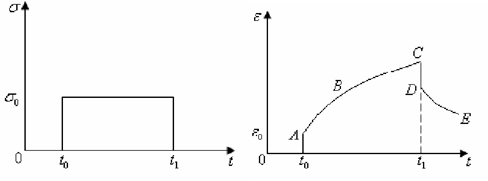
\includegraphics[width=0.9\linewidth]{figure/strain}
	    \fcaption{应变蠕变回复曲线}{Creep function}[介质应变蠕变回复曲线]
		\label{fig:strain}
\end{figure*}
\begin{figure*}[!htbp]
	    \centering
		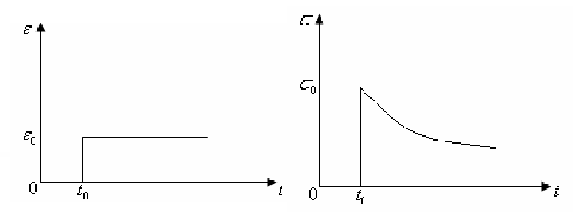
\includegraphics[width=0.95\linewidth]{figure/stress}
	    \fcaption{应力松驰曲线}{Relaxation function}[介质应力松驰曲线]
		\label{fig:stress}
\end{figure*}


\vspace{0.2cm}
\subsection{Maxwell模型}
\vspace{0.2cm}
如图\ref{fig:maxwell_model}所示,弹簧与阻尼器简单的串联即可得到Maxwell模型。对模型施加一个
应力$\sigma$,就会在模型的弹簧中产生形变$\epsilon_1$,并在阻尼器中产生形变$\epsilon_2$。
弹簧中的应力-应变关系为:
\begin{equation}
	\sigma=M_u\epsilon_1,
\end{equation}
其中$M_u$是弹簧的弹性模量,下标$u$表示“无驰豫”。阻尼器中的应力-应变关系为:
\begin{equation}
	\sigma=\eta\partial_t \epsilon_2, \quad \eta\geq0,
\end{equation}
其中$\eta$为粘滞系数。
\begin{figure*}[!htbp]
	    \centering
		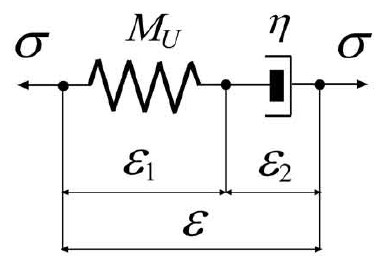
\includegraphics[width=0.6\linewidth]{figure/maxwell_model}
	    \fcaption{Maxwell模型}{Maxwell model}[Maxwell模型]
		\label{fig:maxwell_model}
\end{figure*}
假设系统的总形变量为$\epsilon=\epsilon_1+\epsilon_2$,则Maxwell模型对应的应力-应变关系为:
\begin{equation}
	\frac{\partial_t\sigma}{M_u}+\frac{\sigma}{\eta}=\partial_t\epsilon.
	\label{eq:stress_maxwell}
\end{equation}
对方程(\ref{eq:stress_maxwell})两边做Fourier变换有
\begin{equation}
	\sigma=M\epsilon,
\end{equation}
其中$M(\omega)=\frac{\omega\eta}{\omega\tau-i}$是复模量,并且满足驰豫时间
$\tau=\frac{\eta}{M_u}$。由(\ref{eq:fourier})式可得其相应的驰豫函数为:
\begin{equation}
	\varphi(t)=M_u\exp(-t/\tau)H(t).
\end{equation}
由$M(\omega)J(\omega)=1$可以推到出$Maxwell$模型的蠕变函数,
\begin{equation}
	\chi(t)=\frac{1}{M_u}(1+\frac{t}{\tau})H(t).
\end{equation}
Maxwell模型($M_u=2.16GP_a,\tau=1/(2\pi f),f=25Hz$)的蠕变和驰豫函数如图\ref{fig:maxwell_creep}
所示,蠕变函数并不能代表真实固体中的蠕变行为,而是类似于粘性流体的蠕变函数。
\begin{figure*}[!htbp]
	    \centering
		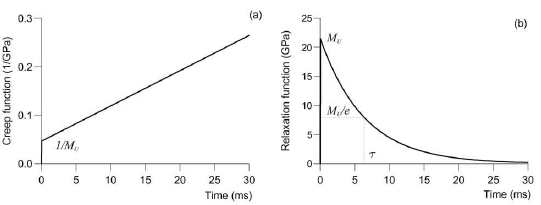
\includegraphics[width=0.9\linewidth]{figure/maxwell_creep}
		\fcaption{Maxwell模型的蠕变(a)和驰豫(b)函数}{The creep and relaxation function 
		of Maxwell model}[Maxwell模型的蠕变和驰豫函数]
		\label{fig:maxwell_creep}
\end{figure*}
在松弛实验中,弹簧和阻尼器受同样大小的力,由于阻尼器不能产生瞬间的形变,因此最初的伸展出现在
弹簧中。阻尼器扩张而弹簧压缩,所以导致模型的总拉伸量相等。最后弹簧中的应力全部释放,而驰豫函数
不像真实固体中的那样呈现双曲关系的剩余应力,所以Maxwell模型适合代表粘滞性流体模型。从图
\ref{fig:maxwell_creep}(a)中可以看出$M_u$代表系统的瞬时响应,所以叫做无驰豫的模量。
地震波的传播属性被介质的相速度、衰减系数以及品质因子所描述。Maxwell模型的品质因子有如下
简单的表达形式:
\begin{equation}
	Q(\omega)=\frac{Re(M)}{Im(M)}=\omega\tau.
\end{equation}
模型($M_u=\rho c^2, \rho=2.4g/cm^3, c=3km/s, \tau=1/(2\pi f), f=25Hz$)的相速度和耗散因子如
图\ref{fig:maxwell_vp}所示。当$\omega\to0$时,$v_p=0$,当$\omega\to\infty$时,$v_p\to\sqrt{M_u/\rho}$
即处于弹性状态。这表明波在Maxwell模型中的传播速度慢于在用弹簧代表的弹性固体中的传播速度。耗散因子
在零频率成分时为无穷大,在高频时表现为无衰减特性。
\begin{figure*}[!htbp]
	    \centering
		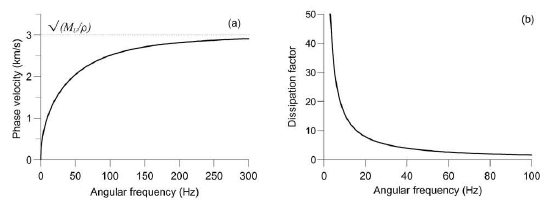
\includegraphics[width=0.8\linewidth]{figure/maxwell_vp}
		\fcaption{Maxwell模型的相速度(a)和耗散因子(b)}{The phase velocity and dissipation factor 
		of Maxwell model}[Maxwell模型的相速度和耗散因子]
		\label{fig:maxwell_vp}
\end{figure*}


\vspace{0.5cm}
\subsection{Kelvin-Voigt模型}
\vspace{0.5cm}
在弹性力学中,通常用Kelvin-Voigt应力-应变关系来描述粘弹介质模型,其模型由弹簧和阻尼器并联而成
(图\ref{fig:kelvin_model})
\begin{figure*}[!htbp]
	    \centering
		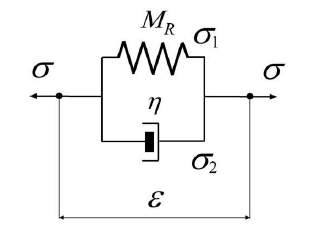
\includegraphics[width=0.6\linewidth]{figure/kelvin_model}
	    \fcaption{Kelvin-Voigt模型}{Kelvin-Voigt model}[Kelvin-Voigt模型]
		\label{fig:kelvin_model}
\end{figure*}
总的应力可以分解成弹性应力与粘性应力:
\begin{equation}
	\left\lbrace
	\begin{aligned}
		\sigma_1=M_R\epsilon, \\
		\sigma_2=\eta\partial_t\epsilon,
	\end{aligned} \right
\end{equation}
其中$M_R$为弹簧模量,下标$R$表示“驰豫”,$\epsilon$为系统的总应变。其应力-应变关系为
\begin{equation}
	\sigma=\sigma_1+\sigma_2=M_R\epsilon+\eta\partial_t\epsilon.
	\label{eq:kelvin}
\end{equation}
对(\ref{eq:kelvin})式做Fourier变换有:
\begin{equation}
	\sigma=(M_R+i\omega\eta)\epsilon,
\end{equation}
即可得出复模量为$M(\omega)=M_R+i\omega\eta$。
Kelvin-Voigt模型的驰豫函数为:
\begin{equation}
	\varphi(t)=M_RH(t)+\eta\delta(t),
\end{equation}
其蠕变函数为:
\begin{equation}
	\chi(t)=\frac{1}{M_R}[1-\exp(-t/\tau)]H(t),
\end{equation}
其中$\tau=\eta/M_R$。

Kelvin-Voigt模型($M_R=2.16GP_a,\tau=1/(2\pi f),f=25Hz$)的驰豫函数和蠕变函数如图\ref{fig:kelvin_creep}
所示。驰豫函数与时间无关,这是一种存弹性固体。$\delta$函数表明在实际中对介质施加一个瞬时应变是不可能的。
阻尼器最先开始拉伸然后转换成应力存储于弹簧中。最后,剩余应力都存储于弹簧中。阻尼器不能瞬间移动导致蠕变
函数不能表示瞬时应变。这不是真实的固体介质,蠕变函数当时间趋于无穷时趋近于驰豫模量$M_R$。
\begin{figure*}[!htbp]
	    \centering
		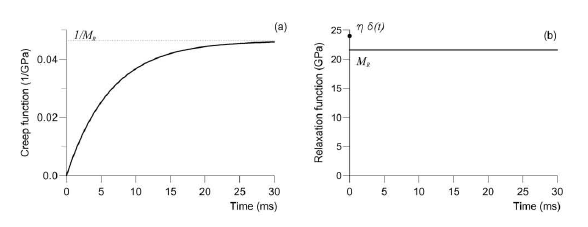
\includegraphics[width=0.9\linewidth]{figure/kelvin_creep}
		\fcaption{Kelvin-Voigt模型的蠕变(a)和驰豫(b)函数}{The creep and relaxation function 
		of Kelvin-Voigt model}[Kelvin-Voigt模型的蠕变和驰豫函数]
		\label{fig:kelvin_creep}
\end{figure*}
\begin{figure*}[!htbp]
	    \centering
		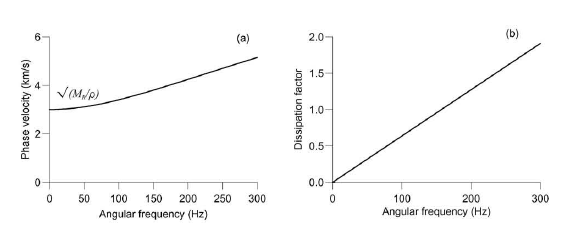
\includegraphics[width=0.8\linewidth]{figure/kelvin_vp}
		\fcaption{Kelvin-Voigt模型的相速度(a)和耗散因子(b)}{The phase velocity and dissipation factor 
		of Kelvin-Voigt model}[Kelvin-Voigt模型的相速度和耗散因子]
		\label{fig:kelvin_vp}
\end{figure*}
Kelvin-Voigt模型的品质因子为:
\begin{equation}
	Q(\omega)=(\omega\tau)^{-1}.
\end{equation}
Kelvin-Voigt模型的品质因子于Maxwell模型的品质因子互为倒数。Kelvin-Voigt模型($M_R=\rho c^2,
\rho=2.4g/cm^3,c=3km/s,\tau=1/(2\pi f),f=25Hz $)的相速度和耗散因子如图\ref{fig:kelvin_vp}所示。
当$\omega\to0$时,$v_p\to\sqrt{M_R/\rho}$;当$\omega\to\infty$时,$v_p\to\infty$。这表明波
在Kelvin-Voigt模型中的传播速度比在相应的弹性介质中的速度大。


\vspace{0.2cm}
\subsection{Zener模型或标准线性固体模型}
\vspace{0.2cm}
Zener或标准线性固体模型由弹簧跟Kelvin-Voigt模型串联形成(图\ref{fig:sls_model})。该模型更能代表真实介质,如
岩石、聚合物以及金属材料。
\begin{figure*}[!htbp]
	    \centering
		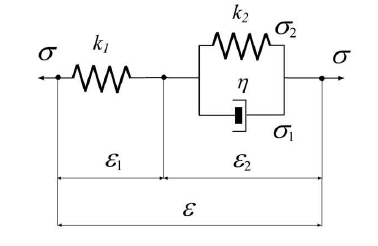
\includegraphics[width=0.6\linewidth]{figure/sls_model}
	    \fcaption{标准线性固体模型}{Standard linear solid model}[标准线性固体模型]
		\label{fig:sls_model}
\end{figure*}
标准线性固体模型的应力-应变关系为:
\begin{equation}
	\left\lbrace
	\begin{aligned}
		\sigma=\kappa_1\epsilon_1, \\
		\sigma_1=\eta\partial_t\epsilon_2, \\
		\sigma_2=\kappa_2\epsilon_2, 
	\end{aligned} \right
\end{equation}
其中$\kappa_1\geq0,\kappa_2\geq0,\eta\geq0$,并且
\begin{equation}
	\sigma=\sigma_1+\sigma_2, \quad \epsilon=\epsilon_1+\epsilon_2.
\end{equation}
上述方程的解给出了标准线性固体模型的应力-应变关系:
\begin{equation}
	\sigma+\tau_\sigma\partial_t\sigma=M_R(\epsilon+\tau_\epsilon\partial_t\epsilon),
\end{equation}
其中$M_R=\frac{\kappa_1\kappa_2}{\kappa_1+\kappa_2}$为拉伸模量,驰豫时间满足$\tau_\sigma=
\frac{\eta}{\kappa_1+\kappa_2},\tau_\epsilon=\frac{\eta}{\kappa_2}\geq\tau_\sigma$。
其中复模量为:
\begin{equation}
	M(\omega)=M_R\frac{1+i\omega\tau_\epsilon}{1+i\omega\tau_\sigma},
\end{equation}
驰豫模量$M_R$由$\omega=0$时得到,未驰豫模量$M_U$由$\omega\to\infty$时得到,且为$M_U=M_R
\frac{\tau_\epsilon}{\tau_\sigma}$。
标准线性固体模型的驰豫函数为:
\begin{equation}
	\varphi(t)=M_R[1-(1-\frac{\tau_\epsilon}{\tau_\sigma})\exp(-t/\tau_\sigma)]H(t),
\end{equation}
其蠕变函数为:
\begin{equation}
	\chi(t)=\frac{1}{M_R}[1-(1-\frac{\tau_\epsilon}{\tau_\sigma})\exp(-t/\tau_\epsilon)]H(t).
\end{equation}
标准线性固体模型($M_R=2.16GP_a,M_U=29.4GP_a,\tau_0=1/(2\pi f),f=25Hz$)的驰豫函数和蠕变函数
如图\ref{fig:sls_creep}所示。
\begin{figure*}[!htbp]
	    \centering
		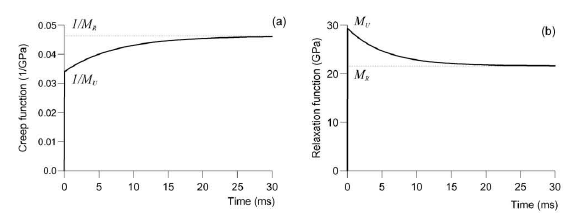
\includegraphics[width=0.9\linewidth]{figure/sls_creep}
		\fcaption{标准线性固体模型的蠕变(a)和驰豫(b)函数}{The creep and relaxation function 
		of standard linear solid model}[标准线性柜台模型的蠕变和驰豫函数]
		\label{fig:sls_creep}
\end{figure*}
\begin{figure*}[!htbp]
	    \centering
		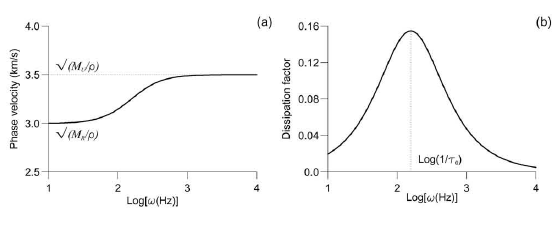
\includegraphics[width=0.8\linewidth]{figure/sls_vp}
		\fcaption{标准线性固体模型的相速度(a)和耗散因子(b)}{The phase velocity and dissipation factor 
		of standard linear solid model}[标准线性固体模型的相速度和耗散因子]
		\label{fig:sls_vp}
\end{figure*}
在蠕变实验中,蠕变由一个由弹簧常数决定的瞬间初始值$\chi(0^+)=M_U^{-1}$逐渐达到其渐进逼近值
$\chi(\infty)=M_R^{-1}$。经过一个初始位移后,应力由于阻尼器变形的增加而逐渐降低,最终使应变达到逼近值。
类似地,驰豫函数经过短暂的处于拉伸状态的$M_U$后,最终达到拉伸模量$M_R$。
标准线性固体模型的品质因子为:
\begin{equation}
	Q(\omega)=\frac{1+\omega^2\tau_\epsilon\tau_\sigma}{\omega(\tau_\epsilon-\tau_\sigma)}.
\end{equation}
标准线性固体模型($M_R=\rho c_R^2,\rho=2.4g/cm^3,c_R=3km/s,M_U=\rho c_U^2,c_U=3.5km/s,f=25Hz$)的
相速度和耗散因子$Q^{-1}$如图\ref{fig:sls_vp}所示。
模型在$\omega_0=1/\tau_0$处有拉伸峰值,其中$\tau_0=\sqrt{\tau_\epsilon\tau_\sigma}$。相速度随着频率的增加
而增加,且在低频时的$\sqrt{M_R/\rho}$与高频时的$\sqrt{M_U/\rho}$之间变化,当介质为纯弹性体($Q^{-1}=0$)
时,$M_R=M_U$。



\vspace{0.9cm}
\subsection{广义Zener模型/近似常$Q$模型}
\vspace{0.1cm}
在油气勘探和地震学中,由于不知道衰减与频率的依赖关系,用常$Q$模型刻画岩石的吸收衰减会更方便。物理实验表明
衰减系数在许多频率范围内与频率呈线性关系,即品质因子为常数。通常用多($L$)个Zener模型单元并联在一起组成广义
Zener模型来近似常$Q$模型(图\ref{fig:zener})。
\begin{figure*}[!htbp]
	    \centering
		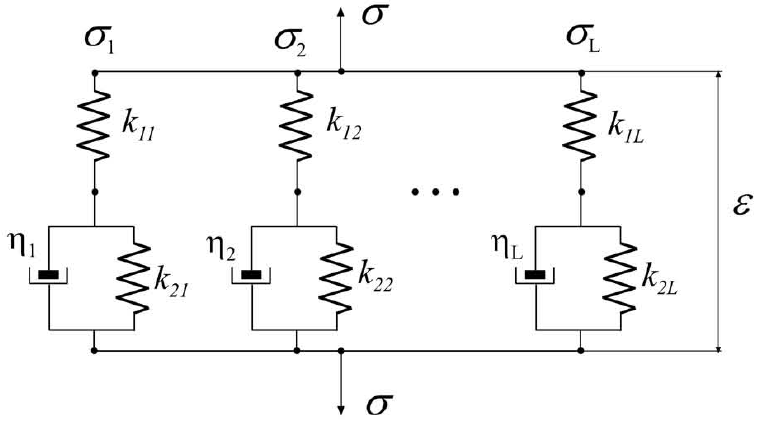
\includegraphics[width=0.7\linewidth]{figure/zener}
	    \fcaption{广义Zener模型}{Generalized Zener model}[广义Zener模型]
		\label{fig:zener}
\end{figure*}
每个小Zener模型单元的应力-应变关系为:
\begin{equation}
	\sigma_l+\tau_{\sigma l}\partial_t\sigma_l=M_{Rl}(\epsilon+\tau_{\epsilon l}
	\partial_t\epsilon), \quad l=1,\cdots L,
\end{equation}
其中驰豫模量为:
\begin{equation}
	M_{Rl}=\frac{\kappa_{1l}\kappa_{2l}}{\kappa_{1l}+\kappa_{2l}},
\end{equation}
驰豫时间为:
\begin{equation}
	\tau_{\sigma l}=\frac{\eta_l}{\kappa_{1l}+\kappa_{2l}}, \quad \tau_{\epsilon l}=
	\frac{\eta_l}{\kappa_{2l}}.
\end{equation}
每个小单元的复模量:
\begin{equation}
	M_l(\omega)=M_{Rl}\frac{1+i\omega\tau_{\epsilon l}}{1+i\omega\tau_{\sigma l}}
\end{equation}
弹性系统的总应力为$\sigma=\sum_{l=1}^{L}\sigma_l$,频率域的应力-应变关系为
\begin{equation}
	\sigma=\sum_{l=1}^{L}M_l\epsilon=\sum_{l=1}^{L}M_{Rl}\frac{1+i\omega\tau_{\epsilon l}}
	{1+i\omega\tau_{\sigma l}}\epsilon.
\end{equation}
选择$M_{Rl}=M_R/L$,复模量可以表示成:
\begin{equation}
	M(\omega)=\sum_{l=1}^{L}M_l(\omega), \quad M_l(\omega)=\frac{M_R}{L}
	(\frac{1+i\omega\tau_{\epsilon l}}{1+i\omega\tau_{\sigma l}})
\end{equation}
由此可以把独立常数减少至$2L+1$个。驰豫函数很容易由时间域的本构关系得到,
\begin{equation}
	\varphi(t)=M_R[1-\frac{1}{L}\sum_{l=1}^{L}(1-\frac{\tau_{\epsilon l}}{\tau_{\sigma l}})
	\exp(-t/\tau_{\sigma l})]H(t),
\end{equation}
当$t=0$时,未驰豫模量为:
\begin{equation}
	M_U=M_R[1-\frac{1}{L}\sum_{l=1}^{L}(1-\frac{\tau_{\epsilon l}}{\tau_{\sigma l}})]
	=\frac{M_R}{L}\sum_{l=1}^{L}\frac{\tau_{\epsilon l}}{\tau_{\sigma l}}.
\end{equation}
单Zener元件的品质因子可以通过中心频率$\omega_0=\tau_0^{-1}$处的品质因子
\begin{equation}
	Q_0=\frac{2\tau_0}{\tau_\epsilon-\tau_\sigma},
	\label{eq:qq}
\end{equation}
表示:
\begin{equation}
	Q(\omega)=Q_0\frac{1+\omega^2\tau_0^2}{2\omega\tau_0}.
\end{equation}
将$\tau_0=\sqrt{\tau_\epsilon\tau_\sigma}$代入方程\ref{eq:qq}中有
\begin{equation}
	\tau_\epsilon=\frac{\tau_0}{Q_0}(\sqrt{Q_0^2+1}+1), \quad \tau_\sigma=\frac{\tau_0}{Q_0}(\sqrt{Q_0^2+1}-1).
\end{equation}
寻找一系列驰豫时间$\tau_{\epsilon l}$和$\tau_{\sigma l}$,使得在给定的中心频率$\omega_{0l}=1/\tau_{0l}$附近品质因子
$Q$呈常数。单驰豫的峰值应均匀分布在$log(\omega)$尺度内,整个系统的品质因子为:
\begin{equation}
	Q(\omega)=\frac{Re(M)}{Im(M)}=\frac{Re(\sum_{l=1}^{L}M_l)}{Im(\sum_{l=1}^{L}M_l)}.
\end{equation}
\begin{figure*}[!htbp]
	    \centering
		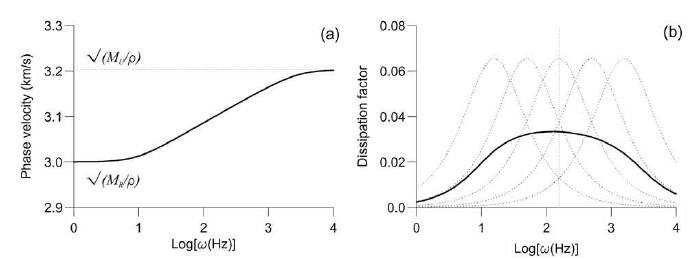
\includegraphics[width=0.8\linewidth]{figure/zener_vp}
		\fcaption{广义Zener模型的相速度(a)和耗散因子(b)}{The phase velocity and dissipation factor 
		of generalied Zener model}[广义Zener模型的相速度和耗散因子]
		\label{fig:zener_vp}
\end{figure*}
\begin{figure*}[!htbp]
	    \centering
		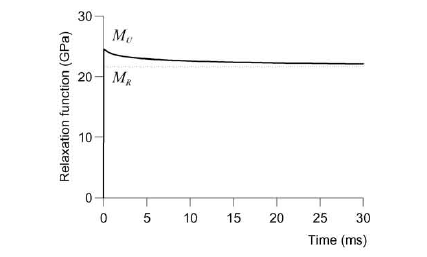
\includegraphics[width=0.7\linewidth]{figure/zener_rela}
		\fcaption{广义Zener模型的驰豫函数}{The relaxation function 
		of standard linear solid model}[广义Zener模型的驰豫函数]
		\label{fig:zener_rela}
\end{figure*}
图\ref{fig:zener_vp}显示了5个Zener单元的相速度和衰减系数随频率的变化关系,其品质因子为30,其中每个单元的
品质因子参数为$Q_0=15$。点划线表示每个单元的品质因子,竖直点划线为第三个单元的驰豫峰值。该近似常$Q$模型的
驰豫函数如图\ref{fig:zener_rela}所示。


\vspace{0.5cm}
\subsection{常$Q$模型}
\vspace{0.5cm}
对所有的频率段,都可以设计出非常理想的常$Q$模型。在勘探地震频段\citeA{kjartansson:1979}提出了基于
蠕变函数$t^{2\gamma}$形式的常$Q$模型,式中$t$是时间,对于地震应用来说$\gamma<<1$。这种模型完全可以用
对应于参考频率的相速度和$Q$两个参数来描述。因此,在数学表达上常$Q$模型要比任何近似常$Q$模型简单。
由于其简单性,Kjartansson常$Q$模型在地震勘探领域有许多应用,尤其是在频率域。
常$Q$模型的驰豫函数为:
\begin{equation}
	\varphi(t)=\frac{M_0}{\Gamma(1-2\gamma)}(\frac{t}{t_0})^{-2\gamma}H(t),
\end{equation}
其中$M_0$是体模量,$\Gamma$是欧拉伽马函数,$t_0$是参考时间,$\gamma$是一个无量刚的参数。
由(\ref{eq:fourier})式可得复模量:
\begin{equation}
	M(\omega)=M_0(\frac{i\omega}{\omega_0})^{2\gamma},
\end{equation}
式中$\omega_0=1/t_0$是参考频率。由(\ref{eq:vc})式可以得出复速度$v_c=\sqrt{\frac{M}{\rho}}$,
其相速度可由(\ref{eq:phase_velocity})式得到$v_p=c_0|\frac{\omega}{\omega_0}|^\gamma$,其中$c_0=
\sqrt{\frac{M_0}{\rho}}[\cos(\frac{\pi\gamma}{2})]^{-1}$。由(\ref{eq:alpha})式可得衰减
系数为$\alpha=\tan(\frac{\pi\gamma}{2})sgn(\omega)\frac{\omega}{v_p}$,并由(\ref{eq:qm})式
可得其品质因子为:
\begin{equation}
	Q=\frac{1}{\tan(\pi\gamma)}.
\end{equation}
首先,根据相速度表达式可得$c_0$是相速度在$\omega=\omega_0$(参考频率)处的值,并且有
\begin{equation}
	M_0=\rho c_0^2\cos^2(\frac{\pi\gamma}{2}).
\end{equation}
其次,$Q$与频率无关,
\begin{equation}
	\gamma=\frac{1}{\pi}\tan^{-1}(\frac{1}{Q}),
\end{equation}
可以表征衰减等级。$Q>0$等同于$0<\gamma<1/2$。

\vspace{0.5cm}
\section{衰减介质地震波传播模拟}
\vspace{0.5cm}
地下介质普遍存在粘滞性,地震波对粘滞性的响应表现为振幅的衰减和速度频散。为了得到精确的成像结果以及
可靠的振幅信息,在进行成像和反演时必须要考虑衰减对地震波传播的影响。波动方程数值模拟是地震成像和反演
的引擎,所以波动方程的推到和求解至关重要。首先波动方程要能准确描述波在特定介质中的传播规律,其次
对波动方程的求解要稳定高效,最后推导出的波动方程还要便于施加边界条件。本节主要推导两类常用的描述衰减性模型
的粘声波动方程,并给出相应的数值解,最后比较这两类粘声波动方程在地震成像中的应用。

\subsection{SLS模型波动方程模拟}
地震波在粘声介质中的传播方程是基于动量守恒以及描述介质流变力学关系的应力-应变关系推导的。标准线性
固体模型的流变力学关系是描述驰豫函数响应的出发点。\citeA{fung:1965},,\citeA{hudson:1980}, 等对标准线性固体模型的
驰豫响应函数给出了详细的描述,并把其应用到了地球介质流变力学解释。

对于二维固体,其动量守恒方程可描述为:
\begin{equation}
	\frac{\partial\sigma_{ji}}{\partial x_j}=\rho\ddot{u}_i+f_i \quad i,j=1,2,
	\label{eq:dl}
\end{equation}
式中$x_j$表示笛卡尔坐标,$u_i(x_k,t)$是位移矢量,$\sigma_{ji}(x_k,t)$是应力张量,$\rho(x_k)$是介质密度
,$f_i(x_k,t)$表示体力。变量上的点表示对时间求偏导,为了简化公式形式,默认使用爱因斯坦求和准则。

在一般声学介质中,应力张量分量可以表示为:
\begin{equation}
	\sigma_{ij}=-p\delta_{ij},
	\label{eq:dl1}
\end{equation}
式中$p(x_k,t)$是介质的压力场。把(\ref{eq:dl})式带入(\ref{eq:dl1})式有:
\begin{equation}
	-\frac{\partial p}{\partial x_i}=\rho\ddot{u}_i+f_i 
	\label{eq:dl3}
\end{equation}
方程(\ref{eq:dl3})两边同时除以密度并求散度得:
\begin{equation}
	-\frac{\partial }{\partial x_i}(\frac{1}{\rho}\frac{\partial p}{\partial x_i})=\ddot{e}+s, 
	\label{eq:dl4}
\end{equation}
其中
\begin{equation}
	e=\frac{\partial u_i}{x_i}=e_{ii},
\end{equation}
是应变张量的迹或者体应变,并且有:
\begin{equation}
	s=\frac{\partial}{\partial x_i}({\frac{1}{\rho}f_i).
\end{equation}
\citeA{christensen:1982},提出了含有多个驰豫力学模型的标准线性固体粘声介质的应力-应变关系:
\begin{equation}
	\sum_{k=0}^mc_k\frac{d^kp}{dt^k}=\sum_{k=0}^md_k\frac{d^ke}{dt^k} \quad m\in N,
	\label{eq:stra1}
\end{equation}
式中$d^k/dt^k$表示$k$阶时间偏导数,$c_k$和$d_k$是介质属性的系数,并且满足如下初始条件:
\begin{equation}
	\sum_{k=0}^mc_rp^{r-k}(0)=\sum_{r=k}^md_re^{r-k}(0),
\end{equation}
其中$p^{r-k}(0)$和$e^{r-k}(0)$分别表示压力和体应变在$t=0$时刻的$(r-k)$阶时间偏导数。通过拉普拉斯
变换求解方程(\ref{eq:stra1})可得到压力场的显示表达式:
\begin{equation}
	p(t)=-M_R\int_{-\infty}^{t}\dot{e}(\tau)[1-\sum_{l=1}^L(1-\frac{\tau_{\epsilon l}}{\tau_{\sigma l}})
	\exp(-\frac{t-\tau}{\tau_{\sigma l}})]d\tau,
	\label{eq:pressure}
\end{equation}
式中$\tau_{\sigma l}(x_k)$和$\tau_{\epsilon l}(x_k)$表示材料第$l$个力学小单元的驰豫时间,$L$是力学机制模型
的个数,$M_R(x_k)$是介质的驰豫模量。方程(\ref{eq:pressure})是Boltzman叠加原理的数学表达形式,它表示当前
压力是先前所有时间压力影响的叠加。

方程(\ref{eq:dl4})和(\ref{eq:pressure})描述了粘声介质的形变,并且可以基于此方程来求取数值解。
然而方程(\ref{eq:pressure})中的褶积运算需要知道应变在整个时间上的值而使得数值求解变得困难。而且,方程
(\ref{eq:stra1})很难直接应用。因此,\citeA{carcione:1988},提出了记忆变量方法来解决方程(\ref{eq:pressure})
中褶积运算遇到的问题。通过引入记忆变量,方程(\ref{eq:pressure})中的褶积计算就可以避免。整合
方程(\ref{eq:pressure})得:
\begin{equation}
	p(t)=-e(t)M_R[1-\sum_{l=1}^L(1-\frac{\tau_{\epsilon l}}{\tau_{\sigma l}})]-
	\sum_{l=1}^L\int_{-\infty}^{t}e(\tau)\phi_l(t-\tau)d\tau,
	\label{eq:memo}
\end{equation}
式中$\phi_l$表示为:
\begin{equation}
	\phi_l(t)=\frac{M_R}{\tau_{\sigma l}}(1-\frac{\tau_{\epsilon l}}{\tau_{\sigma l}})e^{t/\tau_{\sigma l}}.
	\label{eq:phi1}
\end{equation}
方程(\ref{eq:memo})是物理过程推导出的,不仅仅限于标准线性固体模型,对于其它模型只是$\phi_l$不同
而已。核函数$\phi_l$必须满足如下微分方程:
\begin{equation}
	\dot{\phi}_l(t)=-\phi_l(t)/\tau_{\sigma l}.
	\label{eq:phi2}
\end{equation}
定义$L$个记忆变量$e_{1l}$为:
\begin{equation}
	e_{1l}(t)=\int^t_{-\infty}e(\tau)\phi_l(t-\tau)d\tau \quad l=1,\dots,L.
\end{equation}
由(\ref{eq:phi1})式得
\begin{equation}
	\dot{e}_{1l}(t)=\frac{e_{1l}(t)}{\tau_{\sigma l}}+\phi_l(0)e(t).
	\label{eq:e2}
\end{equation}
应力-应变关系(\ref{eq:memo})可以表示为:
\begin{equation}
	p(t)=-[M_Ue(t)+\sum_{l=1}^Le_{1l}],
	\label{eq:p2}
\end{equation}
式中$M_U$为未驰豫变量,
\begin{equation}
	M_U=M_R[1-\sum_{l=1}^L(1-\frac{\tau_{\epsilon l}}{\tau_{\sigma l}})].
\end{equation}
方程(\ref{eq:dl4}),(\ref{eq:e2})和(\ref{eq:p2})完全控制了地震波在粘声介质中的传播规律。
\citeA{blanch:1995}, 指出,在勘探地震频段内,一个力学驰豫模型即可满足实际应用。因此,对于二维粘声介质,
描述运动和形变的波动方程为:
\begin{equation}
    \begin{aligned}
    \label{eq:visco}
    \frac{\partial v_x}{\partial t} - \frac{1}{\rho}\frac{\partial p}{\partial x}=0,\\
    \frac{\partial v_z}{\partial t} - \frac{1}{\rho}\frac{\partial p}{\partial z}=0,\\
    \frac{\partial p}{\partial t} -
    K\frac{\tau_\epsilon}{\tau_\sigma}(\frac{\partial v_x}{\partial x}+\frac{\partial v_z}{\partial z})-r_p=f(\mathbf{x}_s,t),
    \\
    \frac{\partial{r_p}}{\partial t} +
    \frac{1}{\tau_\sigma}\left[r_p+K(\frac{\tau_\epsilon}{\tau_\sigma}-1)
	(\frac{\partial v_x}{\partial x}+\frac{\partial v_z}{\partial z})]=0.
    \end{aligned}
\end{equation}
式中,$v_x$和$v_z$表示质点在$x$方向和$z$方向的振动速度,$K$是介质的体积模量,驰豫时间$\tau_\sigma$和
$\tau_\epsilon$与介质的品质因子$Q$以及参考频率$f_\omega$有关,
\begin{eqnarray}
    \begin{aligned}
        \tau_\sigma &= \frac{\sqrt{1+\frac{1}{Q^2}}-\frac{1}{Q}}{f_\omega},\\
        \tau_\epsilon &= \frac{1}{f_\omega^2\tau_\sigma}.
    \end{aligned}
\end{eqnarray}
方程(\ref{eq:visco})即为标准线性固体模型所描述的粘声波动方程,此方程可用交错网格有限差分法\citeA{virieux:1984}, ,
\citeA{carcione:1999}, 进行数值求解。

\begin{figure*}[!htbp]
	    \centering
		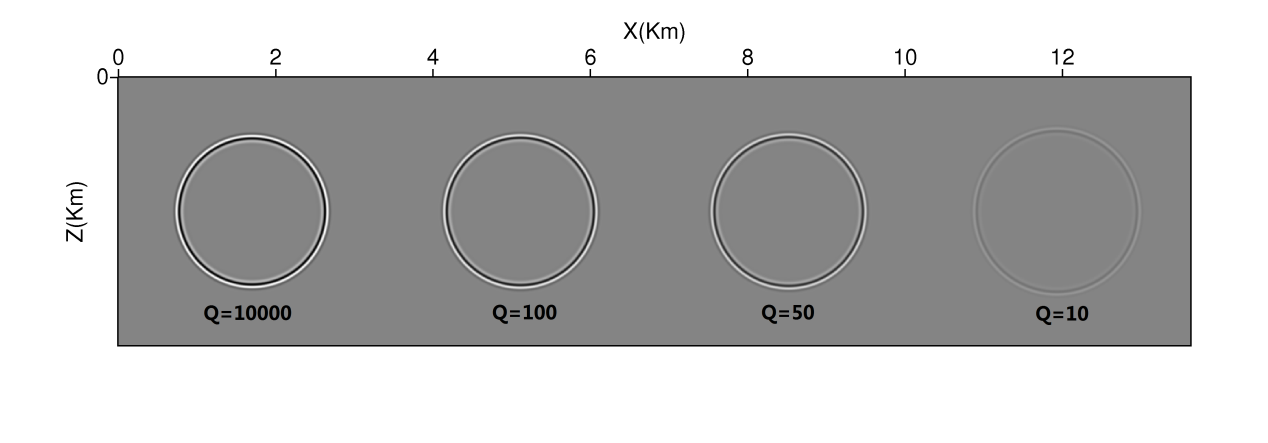
\includegraphics[width=1.0\linewidth]{figure/wave_sls1}
		\fcaption{不同$Q$值在$t=0.35s$的波场快照}{Snapshots of different $Q$  
		models at $t=0.35s$。}[不同$Q$值在$t=0.35s$的波场快照]
		\label{fig:wave_sls1}
\end{figure*}
\begin{figure*}[!htbp]
	    \centering
		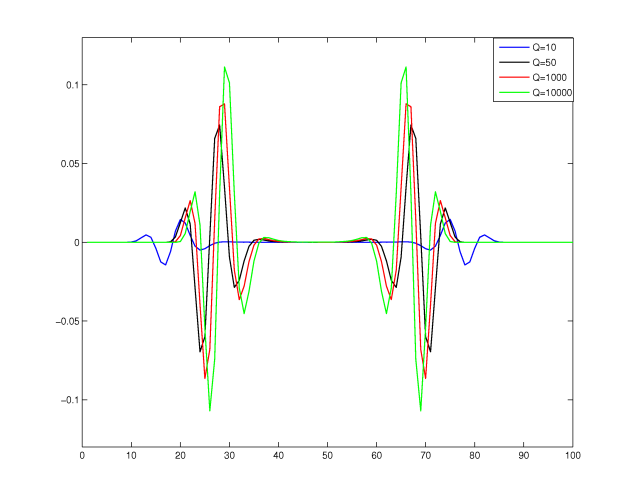
\includegraphics[width=0.5\linewidth]{figure/wave_sls3}
		\fcaption{不同$Q$值在$t=0.35s$,$x=1.7km$处的抽线信息}{The extracted lines  
		of different $Q$ models at $t=0.35s$,$x=1.7km$}[不同$Q$值在$t=0.35s$,$x=1.7km$处的抽线信息]
		\label{fig:wave_sls3}
\end{figure*}
\begin{figure*}[!htbp]
	    \centering
		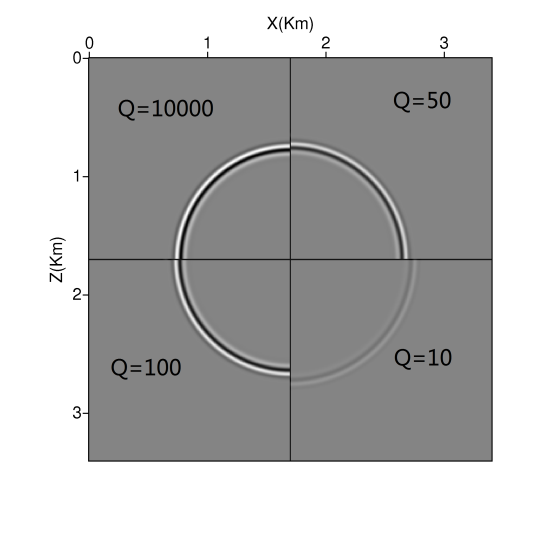
\includegraphics[width=0.5\linewidth]{figure/wave_sls2}
		\fcaption{不同$Q$值在同一时刻波场快照整合图}{Integrated snapshots of different $Q$ 
		model}[不同$Q$值在同一时刻波场快照整合图]
		\label{fig:wave_sls2}
\end{figure*}
\begin{figure*}[!htbp]
	    \centering
		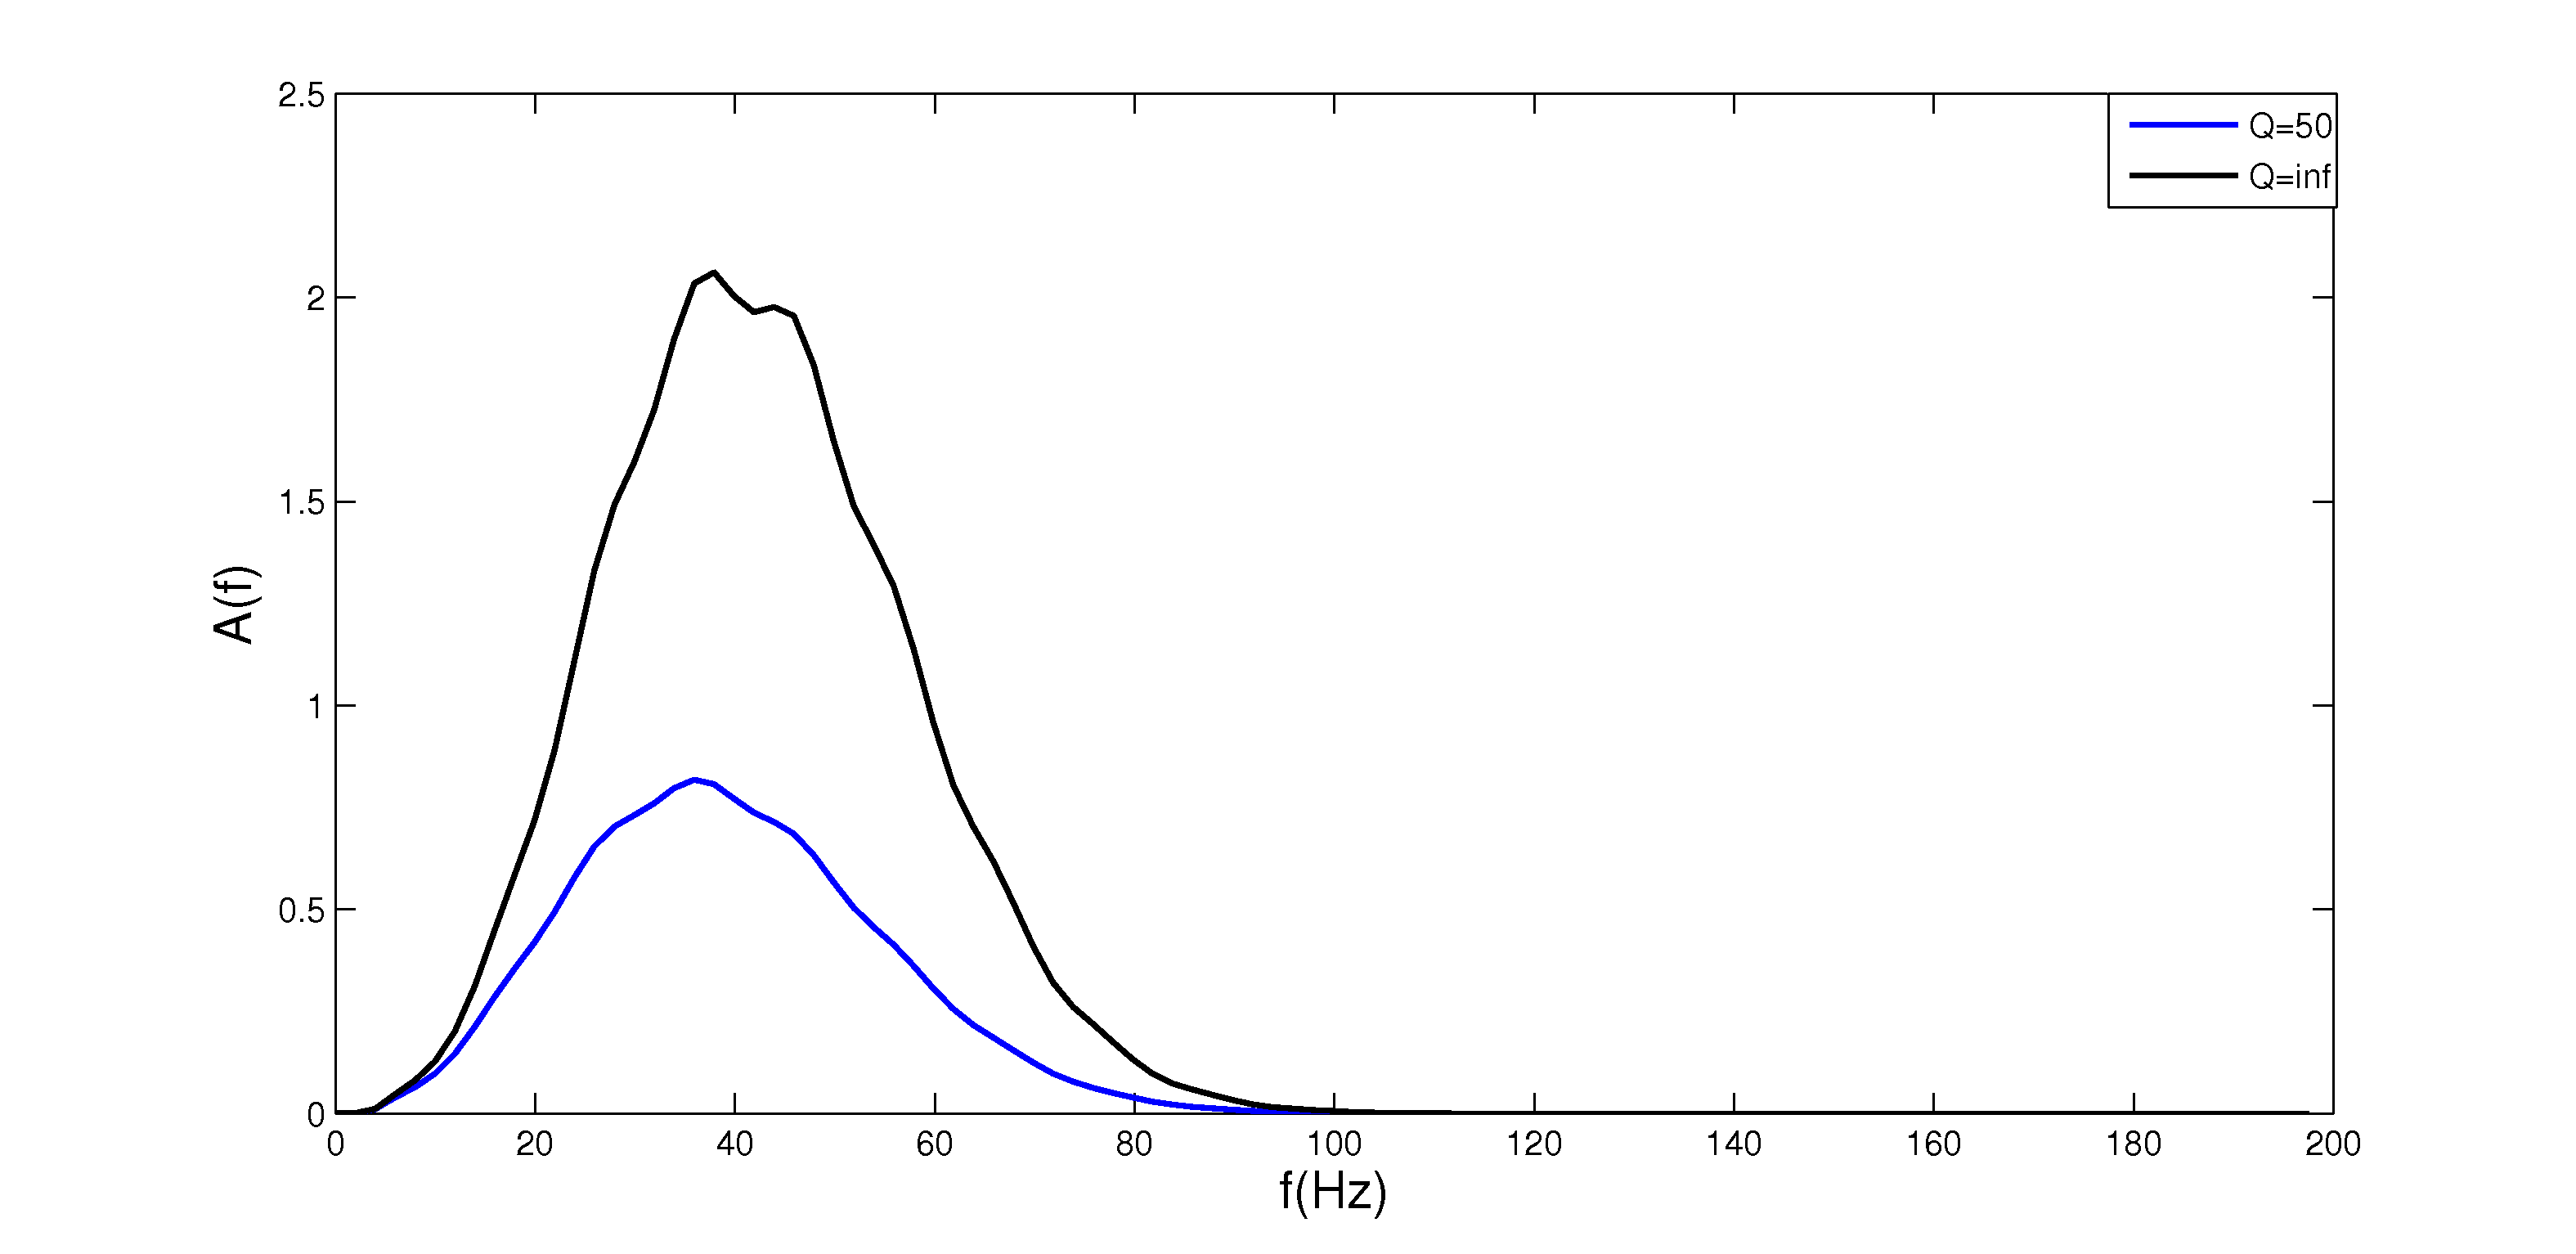
\includegraphics[width=0.7\linewidth]{figure/wave_sls4}
		\fcaption{波场快照抽线的振幅谱}{The amplitude spectrum of extracted lines. 
		}[波场快照抽线的振幅谱]
		\label{fig:wave_sls4}
\end{figure*}
设置一个横向、纵向均为$3.4km$的均匀介质模型,其中纵波速度为$v_p=3km/s$,密度为$\rho=2.0g/cm^3$。
图(\ref{fig:wave_sls1})展示了在$t=0.35s$时刻不同$Q$值的波前快照,图(\ref{fig:wave_sls3})展示
了在$x=1.7km$处的抽线信息,图(\ref{fig:wave_sls2})整合了不同$Q$值的波前快照,图(\ref{fig:wave_sls4})
展示了$Q=50$和声介质波前快照抽线的振幅普。
以上四图从不同的角度证明了粘性介质不仅对地震波振幅有衰减效应而且对相位有较强的改造作用。品质因子的值越小
对地震波的振幅衰减越严重,而且相位有更强的超前效应。从振幅谱可以看出,对高频成分的衰减明显要强于对低频
成分的衰减,这与线性粘弹理论(公式\ref{eq:linear_visco})是一致的。



\vspace{0.5cm}
\subsection{常$Q$模型波动方程模拟}
在勘探地震频段内,认为衰减系数($\alpha\propto 1/Q$)与频率呈近似线性关系,即$Q$在该频段内为常数。
\citeA{kjartansson:1979}, 推导出了常$Q$模型的相速度的频散关系:
\begin{equation}
	c=c_0(\frac{\omega}{\omega_0})^\gamma=c_0^2\cos^2(\pi\gamma/2),
\end{equation}
和衰减系数:
\begin{equation}
	\alpha=\tan(\frac{\pi\gamma}{2})\frac{\omega}{v_p},
\end{equation}
式中$c_0$是在给定的参考频率$\omega_0$处的速度。参数$\gamma=1/\pi\tan^{-1}(1/Q)$是一个无量纲的数,对于
任意正$Q$其取值范围为$0<\gamma<0.5$。\citeA{carcione:2002}推导出了常$Q$模型在时间域的粘声波动方程:
\begin{equation}
	\frac{\partial^{2-2\gamma}p}{\partial t^{2-2\gamma}}=c^2\omega_0^{-2\gamma}\bigtriangledown^2p,
	\label{eq:frac}
\end{equation}
式中$\bigtriangledown^2$是拉普拉斯算子,$p(\mathbf(x),t$是压力波场。方程(\ref{eq:frac})涉及时间的分数
阶偏导数,所以又叫分数阶偏导数方程。在均匀介质中,将波动方程的平面波解
$e^{i(\omega t-\mathbf{k}\cdot\mathbf{x})}$带入方程(\ref{eq:frac})中有如下频散关系:
\begin{equation}
	\frac{\omega^2}{c^2}=(i)^{2\gamma}\omega_0^{-2\gamma}\omega^{2\gamma}\mathbf{k}^2.
	\label{eq:dispersion}
\end{equation}
\citeA{zhu.harris:2014}, 从方程(\ref{eq:dispersion})出发,推导了如下近似频散关系:
\begin{equation}
	\frac{\omega^2}{c^2}=-\eta|\mathbf{k}|^{2\gamma+2}-i\omega\tau|\mathbf{k}|^{2\gamma+1},
	\label{eq:dispersion1}
\end{equation}
对应的分数阶常$Q$波动方程为:
\begin{equation}
	\frac{1}{c_0^2}\frac{\partial^2p}{\partial t^2}=\bigtriangledown^2p + \{\eta(-\bigtriangledown^2)^
	{\gamma+1}-\bigtriangledown^2\}p + \tau\frac{\partial}{\partial t}(-\bigtriangledown^2)^{\gamma+
	\frac{1}{2}}p,
	\label{eq:con_equation}
\end{equation}
其中$\eta=-c_0^{2\gamma}\omega_0^{-2\gamma}\cos(\pi\gamma)$,$\tau=-c_0^{2\gamma-1}\omega^{-2\gamma}
\sin(\pi\gamma)$。方程(\ref{eq:con_equation})中的相速度$c_0$和分数阶指数$\gamma$依赖于空间变量
$\mathbf{x}$,通常是非均匀的,这导致用传统方法求解该方程变得非常困难。近年来,低秩近似方法(\citeA{etgen:2009}, 
,\citeA{cheng.fomel:2014}, )的发展应用使得求解此方程变得容易。用低秩近似求解方程(\ref{eq:con_equation})
的具体实现可参加附录A。另外,\citeA{yao.zhu:2017}, 用埃尔米特分布逼近泛函来求解此方程。


方程(\ref{eq:con_equation})右边有三项,第一项为声波项,第二项控制频散,第三项控制衰减。该方程与方程
(\ref{eq:frac})最主要的区别是显示的把衰减项与频散项显示分开,这对地震波逆时偏移成像有重要意义。
图(\ref{fig:wave_frac})展示了均匀介质模型($Q=10,c_0=2164m/s$),不同控制项产生的波前快照。控制衰减项
产生的波场与声波方程产生的波场具有相同的相位,但是其振幅明显较弱;控制频散项产生的波场与声波方程产生的波场
具有相当的振幅,但是其相位有明显的移动。全粘声方程既衰减了地震波的振幅也改造了地震波的相位。
\begin{figure*}[!htbp]
	    \centering
		
\includegraphics[width=0.5\linewidth]{figure/wave_frac}
		\fcaption{近似常$Q$方程不同控制项产生的波前快照}{Four wavefield parts split by the dashed lines are   
		generated by different formulations。}[近似常$Q$方程不同控制项产生的波前快照]
		\label{fig:wave_frac}
\end{figure*}







\vspace{0.5cm}
\subsection{衰减模型在地震成像中的应用}


%%==================================================
%% chapter03.tex for TJU Master Thesis
%% Encoding: UTF-8
%%==================================================

\chapter{基于粘声方程的反射全波形反演}

对于目前普遍缺乏可靠的低频(小于4Hz)以及长偏移距信息的地震数据,中深层的
参数信息主要包含在反射数据中,常规的FWI对于中深层参数的建模往往无能为力。
因此,反射波波形反演(RWI)成为近几年国际地震勘探领域争相研究的课题。沿
反射波波路径进行背景速度反演已经取得了很多成功的案例。

RWI是处理FWI的强非线性问题的一种有效解决途径,虽然在背景速度建模中被广泛
使用,但是目前为止,尚未有学者将其引入到背景$Q$的估计中。地震衰减对地震波传播
的影响相较于速度对地震波传播的影响既有相似之处,也略有不同。本章将详细介绍
如何把RWI引入到背景$Q$的反演中。

\vspace{1.0cm}
\section{引言}

用地震波信息来反演地下地层的衰减信息已有很多年的研究历史,其反演方法可大致
分为射线层析和波形反演两类。射线层析类方法(\citeA{brzostowski.mcmechan:1992};
\citeA{quan.harris:1997};\citeA{hu.liu:2011})用射线路径来构建层析矩阵,具有很高的
计算效率,对于介质变化简单的情况有很好的应用效果。但当介质复杂时,地震波传播往往
存在多路径,并且当介质存在高速或低速透镜体时,射线追踪会出现焦散现象,不能对其下覆
地层进行很好的照明。波动类的反演方法以全波动方程为传播引擎,能较精确的刻画地震波
在复杂介质中传播的各种波现象,理论上是目前精度最高的参数建模方法。自从
\citeB{lailly:1983}和\citeB{tarantola:1984}等人建立起全波形反演的基本理论框架以来,
越来越多的人关注该方法的研究与应用,尤其是在地震波速度反演方面。在地震品质因子
反演方面,\citeB{tarantola:1988}第一次提出了时间域粘弹波形反演理论。随后,
\citeB{song:1995}在频率域提出了一种粘声波形反演方法($Q$-FWI)。在$Q$-FWI中,速度
参数和品质因子有很强的耦合性(\citeA{song:1995};\citeA{kamei.pratt:2008};
\citeA{hak.mulder:2011})。在观测系统不完备的情况下,解决这中耦合性的思路有
两种,一种是通过预条件模型参数的梯度(\citeA{liao.mcmechan:1996};
\citeA{hak.mulder:2011};\citeA{malinowski:2011})来减弱耦合。另一种是顺序
反演法,先反演对地震数据影响较强的速度参数然后再反演$Q$模型(\citeA{pratt:2004};
\citeA{rao.wang:2008};\citeA{smithyman:2009})。

$Q$-FWI的成功需要低频长偏移距地震数据,但是这种高质量的数据采集需要高昂的采集费用。
当缺少长偏移距的折射数据时,深部模型往往只被反射波照明。因此,利用反射波进行中
深层的速度建模已成为地震成像的共识(\citeA{xu:2012a};\citeA{ma.hale:2013};
\citeA{chi:2015})。但是目前尚未有人用反射波波路径来进行地震衰减建模。本章
在顺序反演的思路下,先假设已获得准确的速度模型,然后引入RWI框架,用反射波来
反演背景$Q$模型。

\vspace{1.0cm}
\section{方法原理}

当利用反射波进行反演时,常规FWI对模型的短波长结构更敏感,而地震衰减对地震数据的
影响是一种沿地震波波路径的累加效应,因而,其长波长的背景模型显得更为重要。RWI通过
将数据残差投影到反射波波路径来构建模型的长波长成分,更加切合对地震衰减参数反演的
需求。本节将介绍粘声反射全波形反演($Q$-RWI)方法原理。

\vspace{1.0cm}
\subsection{反射波波形反演基本思路}

常规的FWI是通过匹配模拟数据和观测数据来推断介质的参数。设$\mathbf{x}_s$和$\mathbf{x}_g$
分别为炮点和检波点的空间位置,时间域FWI最常用的最小平方目标函数为(\citeA{virieux:2009}):
\begin{equation}
    \mathcal{J}(\mathbf{m})=\frac{1}{2}\sum_{s,g}\int_t[d_{obs}(\mathbf{x}_s,\mathbf{x}_g,t)
	        -d_{cal}(\mathbf{x}_s,\mathbf{x}_g,t)]^2dt,
	\label{eq:misfit_function}
\end{equation}
其中$d_{cal}(\mathbf{x}_s,\mathbf{x}_g,t)$是模拟数据,$d_{obs}(\mathbf{x}_s,\mathbf{x}_g,t)$
是观测数据。将目标函数(方程~\ref{eq:misfit_function})在$\mathbf{m}_0$附近进行二阶Taylor展开
有
\begin{equation}
	\mathcal{J}(\mathbf{m}_0+\Delta\mathbf{m})=\mathcal{J}(\mathbf{m}_0)
	+\frac{\partial\mathcal{J}(\mathbf{m}_0)}{\partial\mathbf{m}}\Delta\mathbf{m}
	+\frac{\partial^2\mathcal{J}(\mathbf{m}_0)}{\partial\mathbf{m}^2}\Delta\mathbf{m}^2 
	+ \mathcal{O}(\Delta\mathbf{m}^3).
\end{equation}
当目标函数对模型参数在$\mathbf{m}_0$处的一阶导数等于零时,目标函数取得极小值,即
\begin{equation}
	\Delta\mathbf{m}=-[\frac{\partial^2\mathcal{J}(\mathbf{m}_0)}{\partial\mathbf{m}^2}]^{-1}
	\frac{\partial\mathcal{J}(\mathbf{m}_0)}{\partial\mathbf{m}},
\end{equation}
式中$\frac{\partial\mathcal{J}(\mathbf{m}_0)}{\partial\mathbf{m}}$为梯度方向,$[\frac{\partial^2
\mathcal{J}(\mathbf{m}_0)}{\partial\mathbf{m}^2}]^{-1}$为Hessian的逆。Hessian的逆对反演通常起
照明补偿、加快收敛的作用,但是其计算非常困难,在反演中通常对其做对角近似或常数近似。而一阶梯度
作为目标函数的下降方向显得尤为重要。根据伴随状态法(\citeA{plessix:2006}),目标函数的梯度可用
正传波场与反传的残差波场进行零延迟的互相关得到,即
\begin{equation}
	\frac{\partial\mathcal{J}(\mathbf{m}_0)}{\partial\mathbf{m}} = \mathbf{\lambda}\otimes\mathbf{u},
\end{equation}
其中$\otimes$表示零延迟互相关,$\mathbf{\lambda}$,$\mathbf{u}$分别表示伴随波场和正传波场。
图~\ref{fig:grad_full}展示了两层介质单炮单检波点的常规FWI梯度。其梯度包含四个不同的子梯度
(图~\ref{fig:grad}),
直达波梯度、源端反射波梯度、检波点端反射波梯度以及偏移响应。从图中可以看出不同类型的波
对梯度的贡献量不一样,假设透射波场的振幅为1,背向的反射波的振幅为反射系数的量级$R$(譬如0.1)。
那么梯度中,透射波贡献的能量最强(图~\ref{fig:grad}a),将折射波的数据沿透射波波路径反投影
就可以很好地更新折射波波路径覆盖区域的背景参数,但是这部分能量在深层为零。在FWI的初期阶段
中不合需要的分量是偏移响应(图~\ref{fig:grad}b),其强度为$R$,是由反射波沿折射波波路径投影
得到的。而反演中深部背景参数需要令反射波沿着类似透射形状的反射波路径进行背景参数更新
(图~\ref{fig:grad}c和d),其中兔耳状反射波梯度的强度仅为$R^2$。因此,最需要的兔耳状的
反射波梯度比不合需要的偏移响应的强度还要小一个数量级,如果不采用梯度分解,需要的低波数
能量会被不需要的高波数偏移响应所掩盖,这就是常规FWI通常难以用反射波来更新背景参数的最
主要原因。

\begin{figure*}[!htbp]
	\centering
	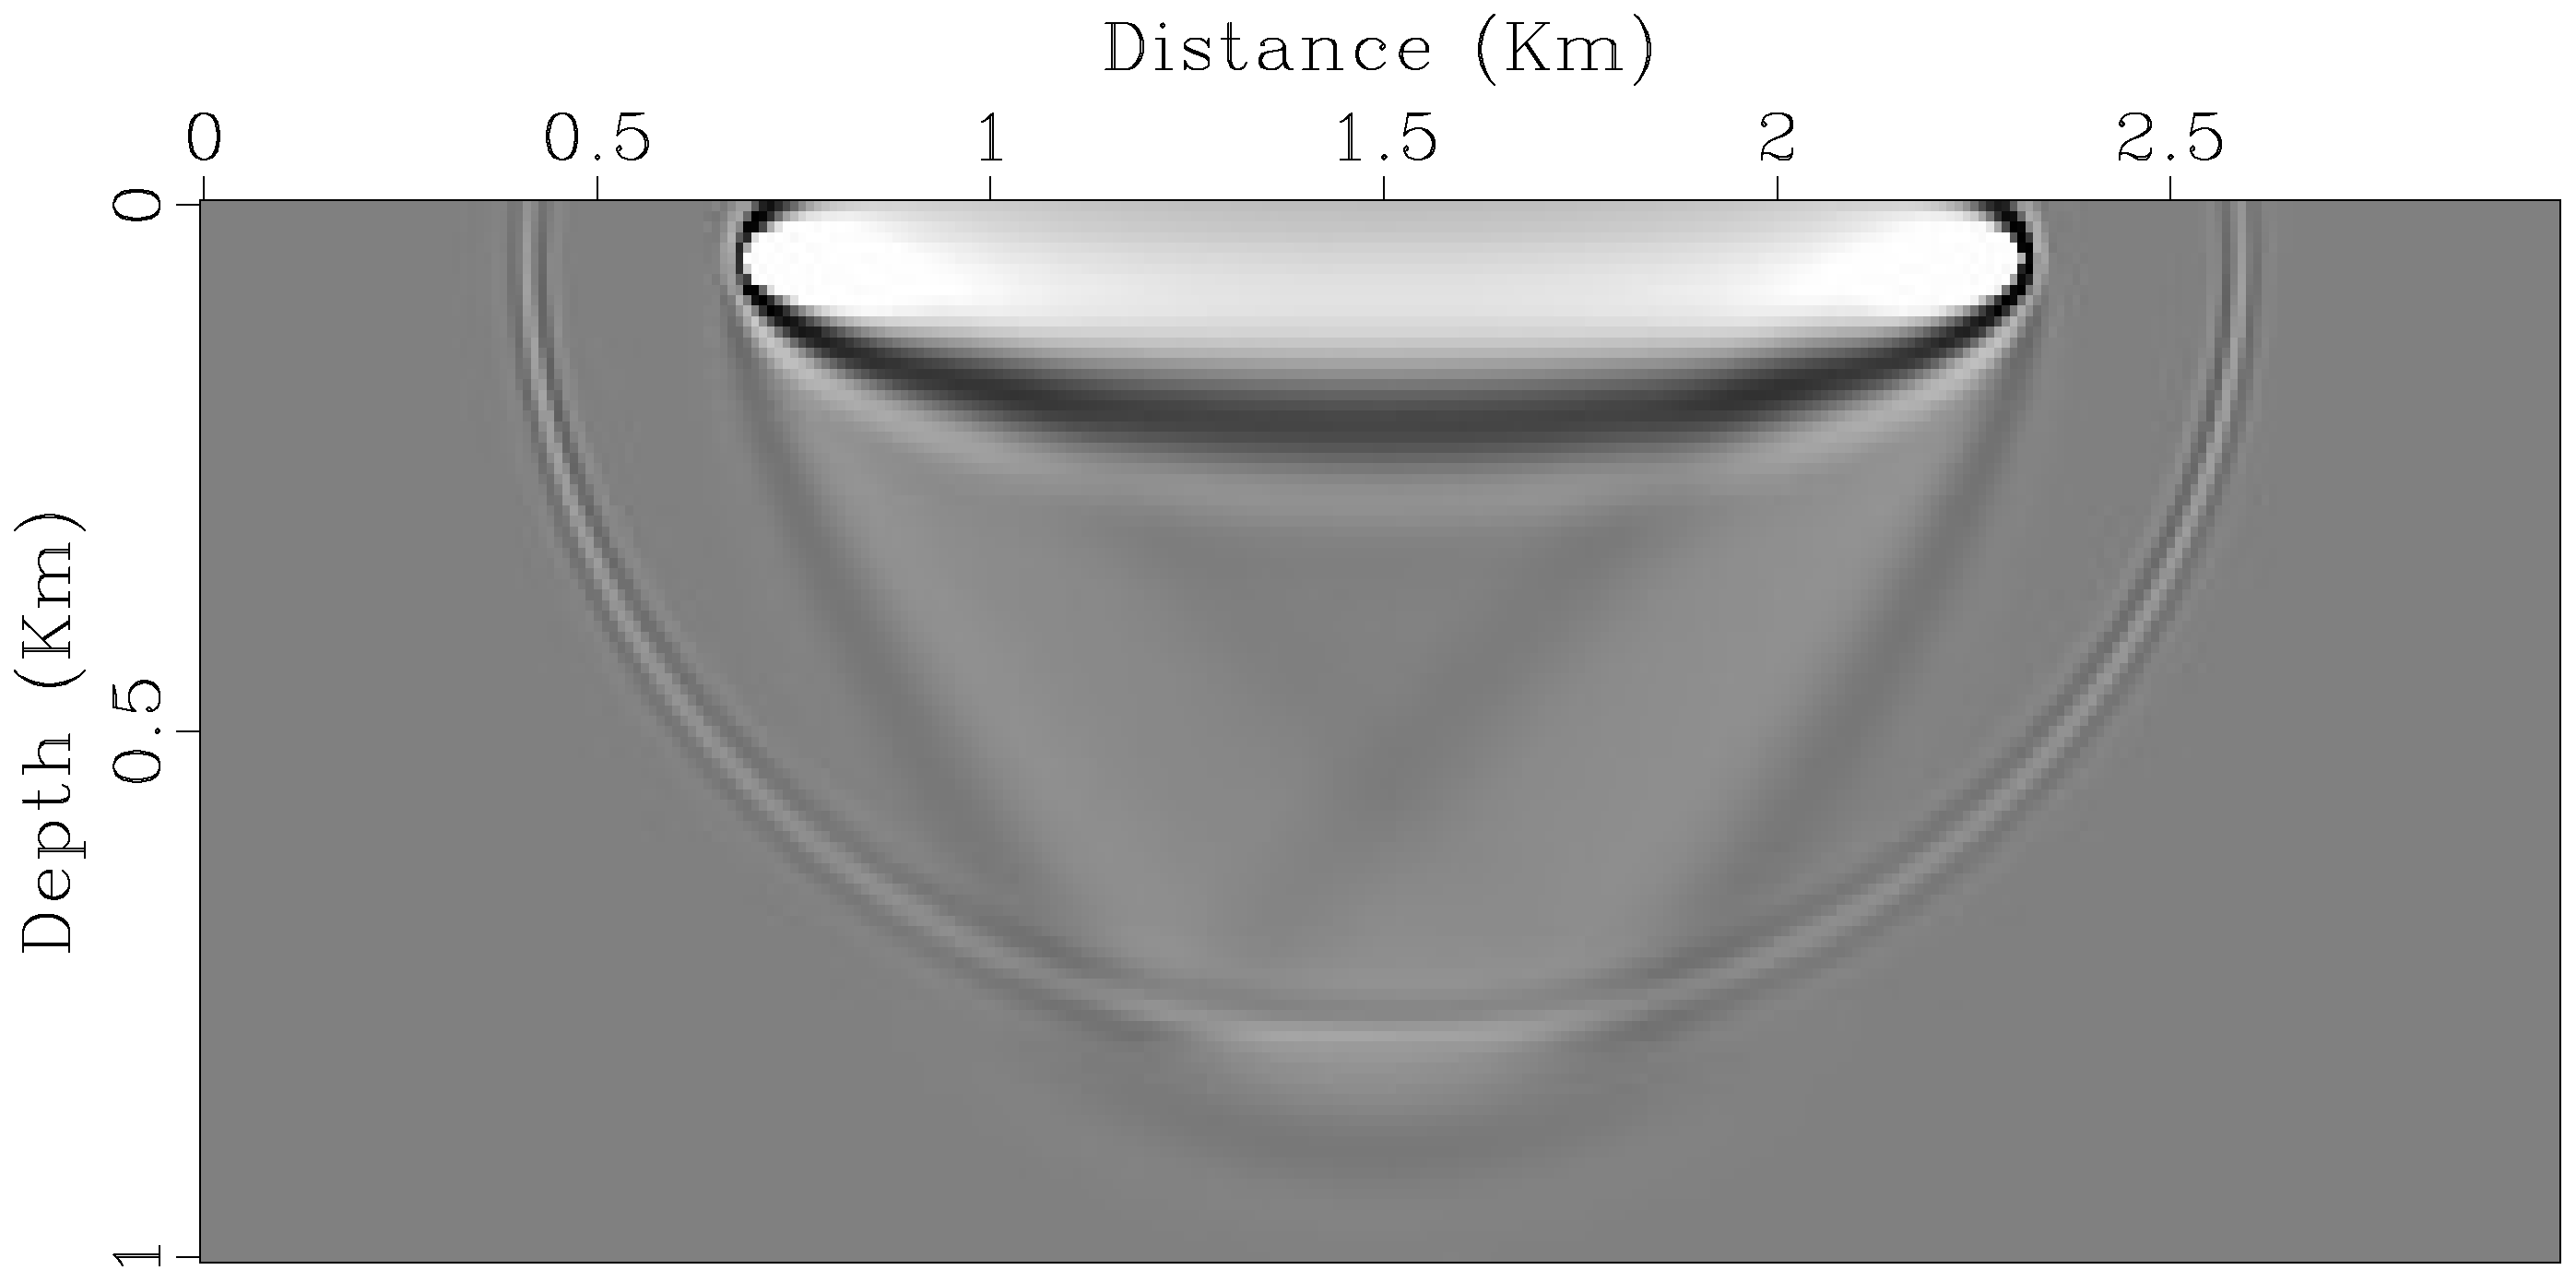
\includegraphics[width=0.95\linewidth]{figure/grad_full}
	\fcaption{两层介质单炮单检波点的FWI梯度。}{The gradient of FWI.
	 }[常规FWI梯度]
	\label{fig:grad_full}
\end{figure*}

\begin{figure*}[!htbp]
	\centering
	\subfigure[]{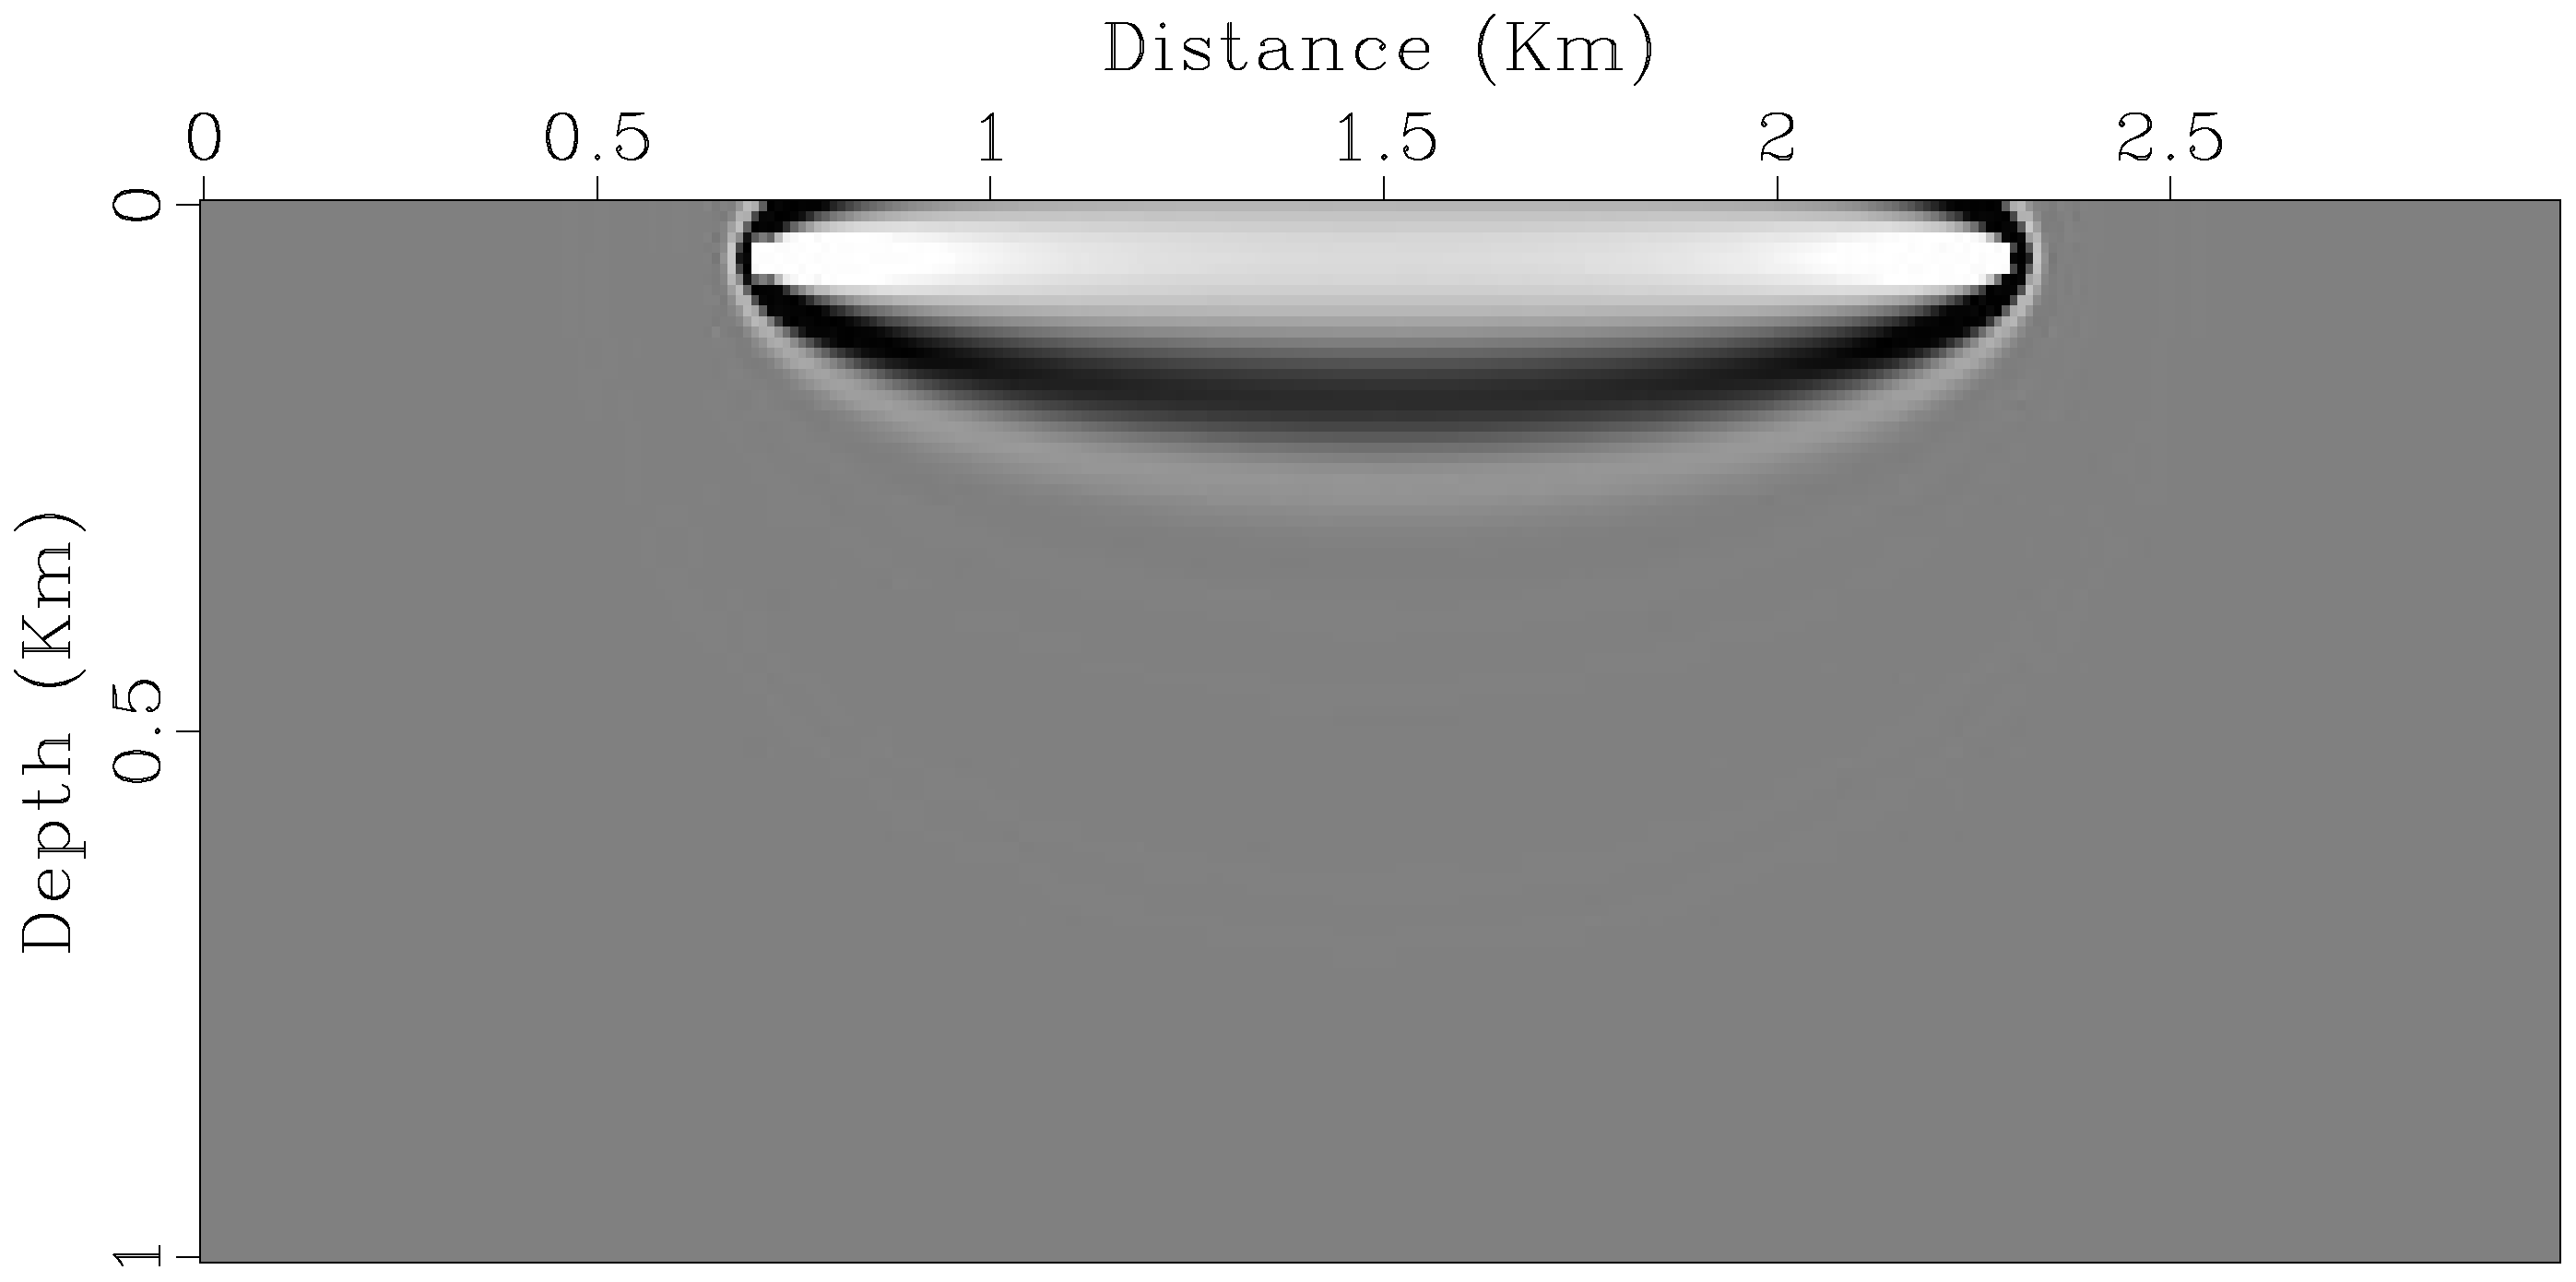
\includegraphics[width=0.45\linewidth]{figure/grad_fwi_dir}}
	\subfigure[]{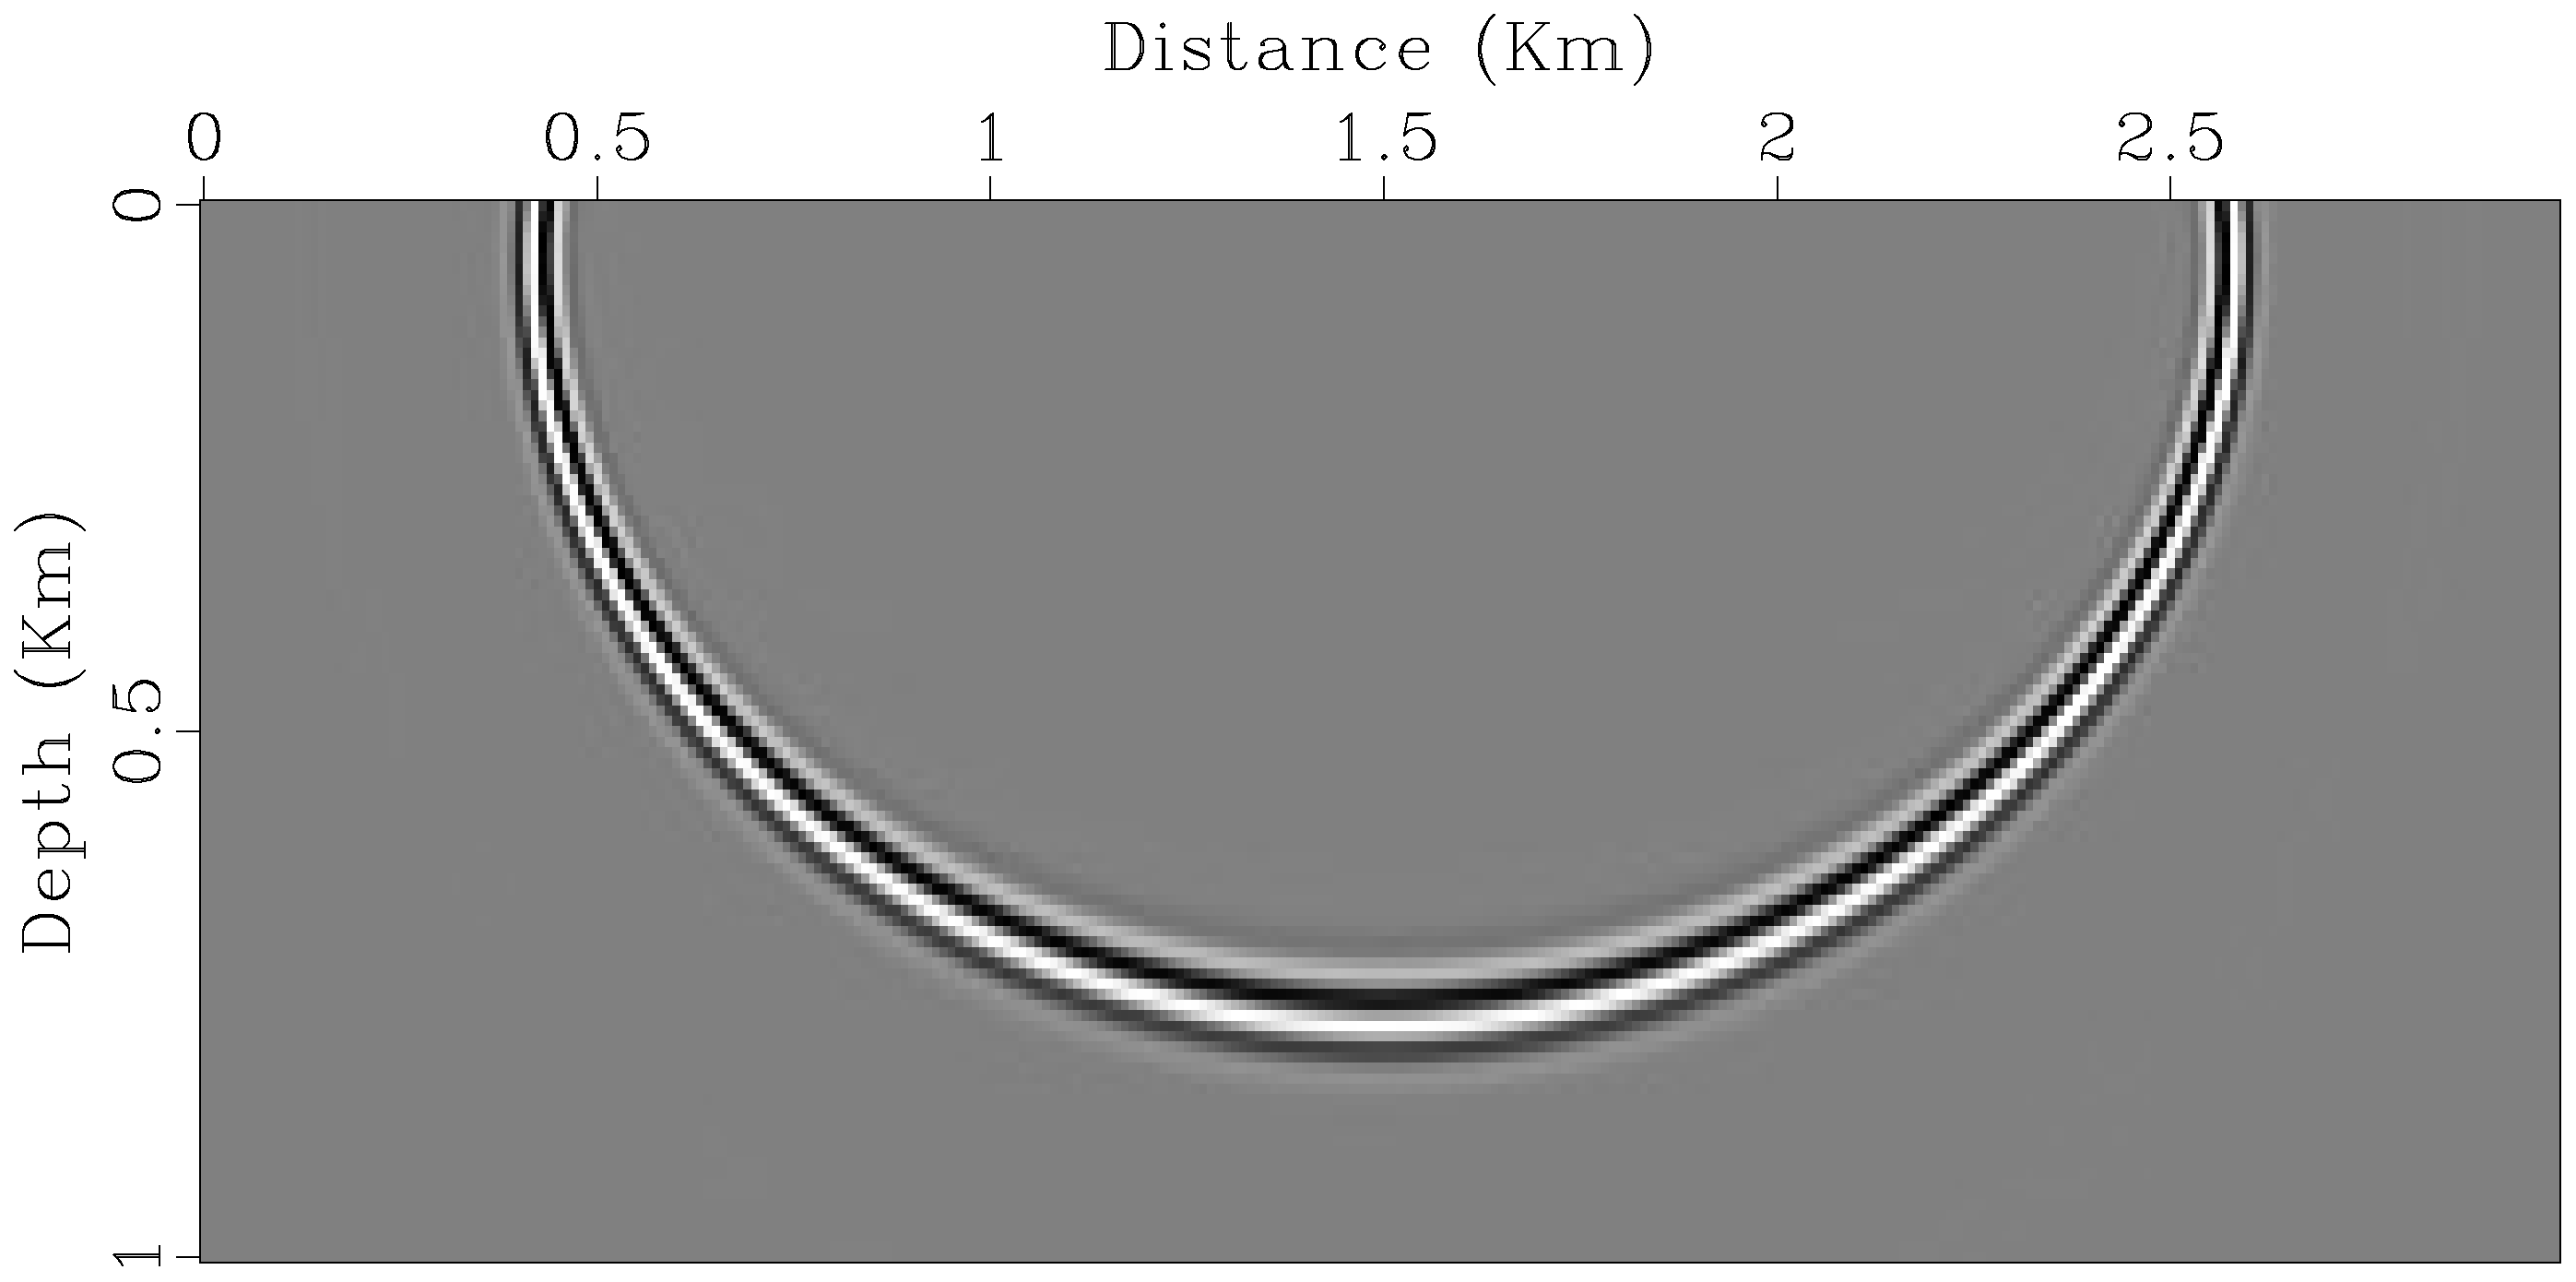
\includegraphics[width=0.45\linewidth]{figure/grad_mig}}
	\subfigure[]{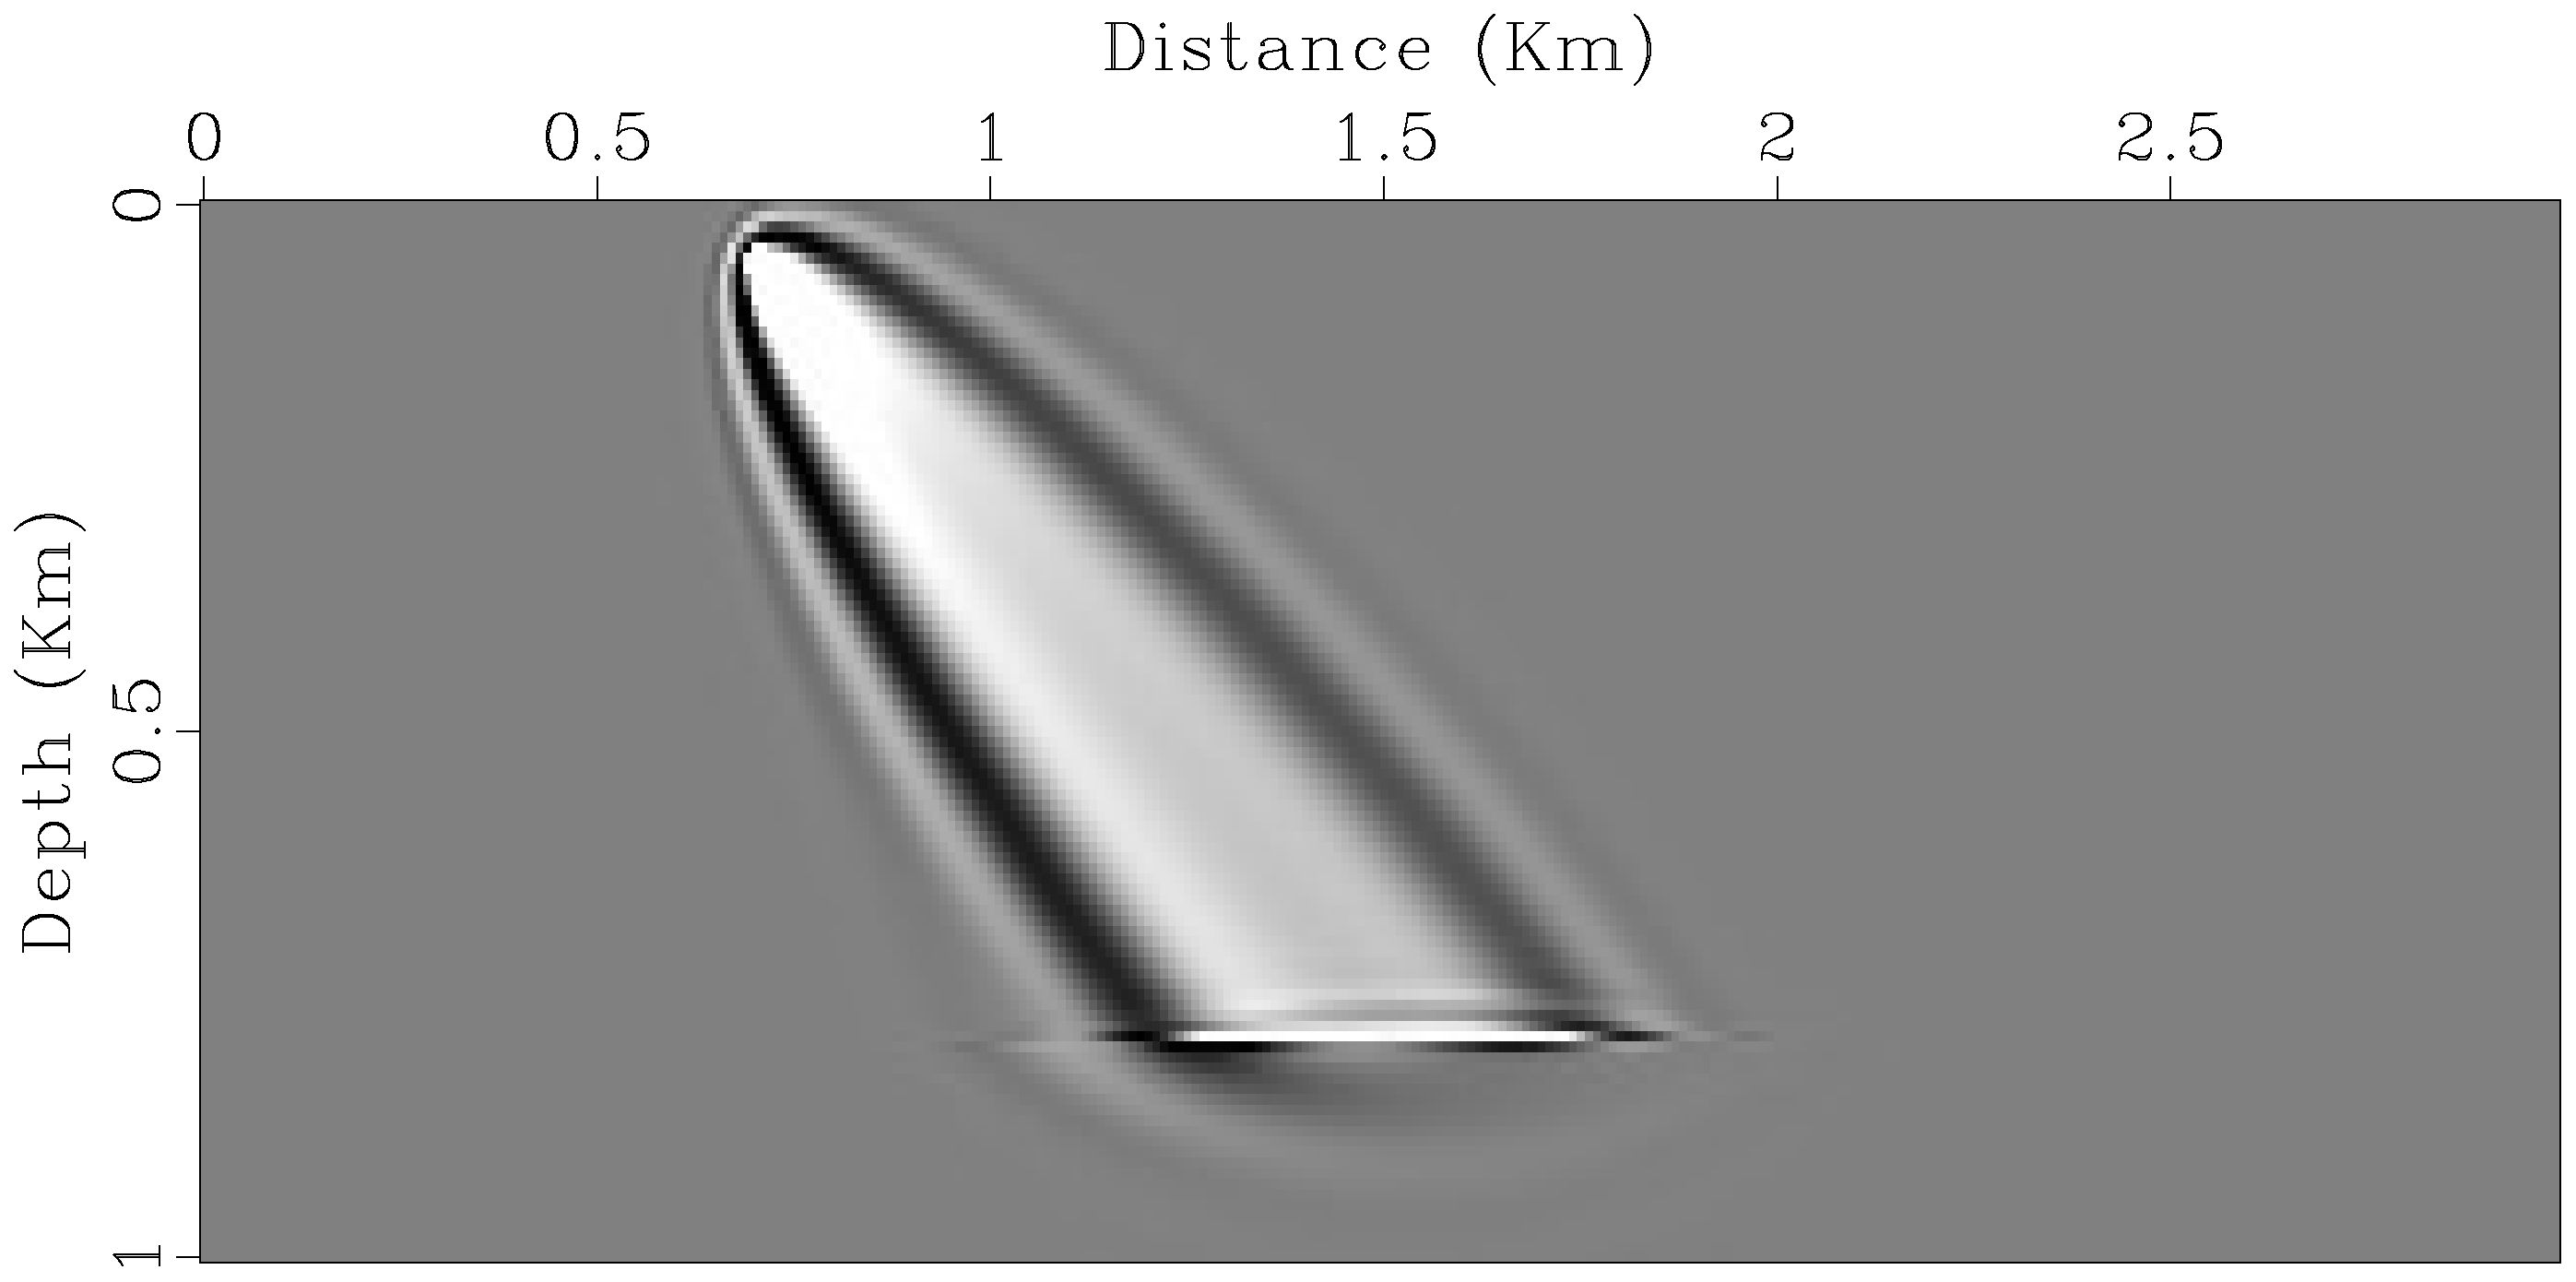
\includegraphics[width=0.45\linewidth]{figure/grads_rwi_one}}
	\subfigure[]{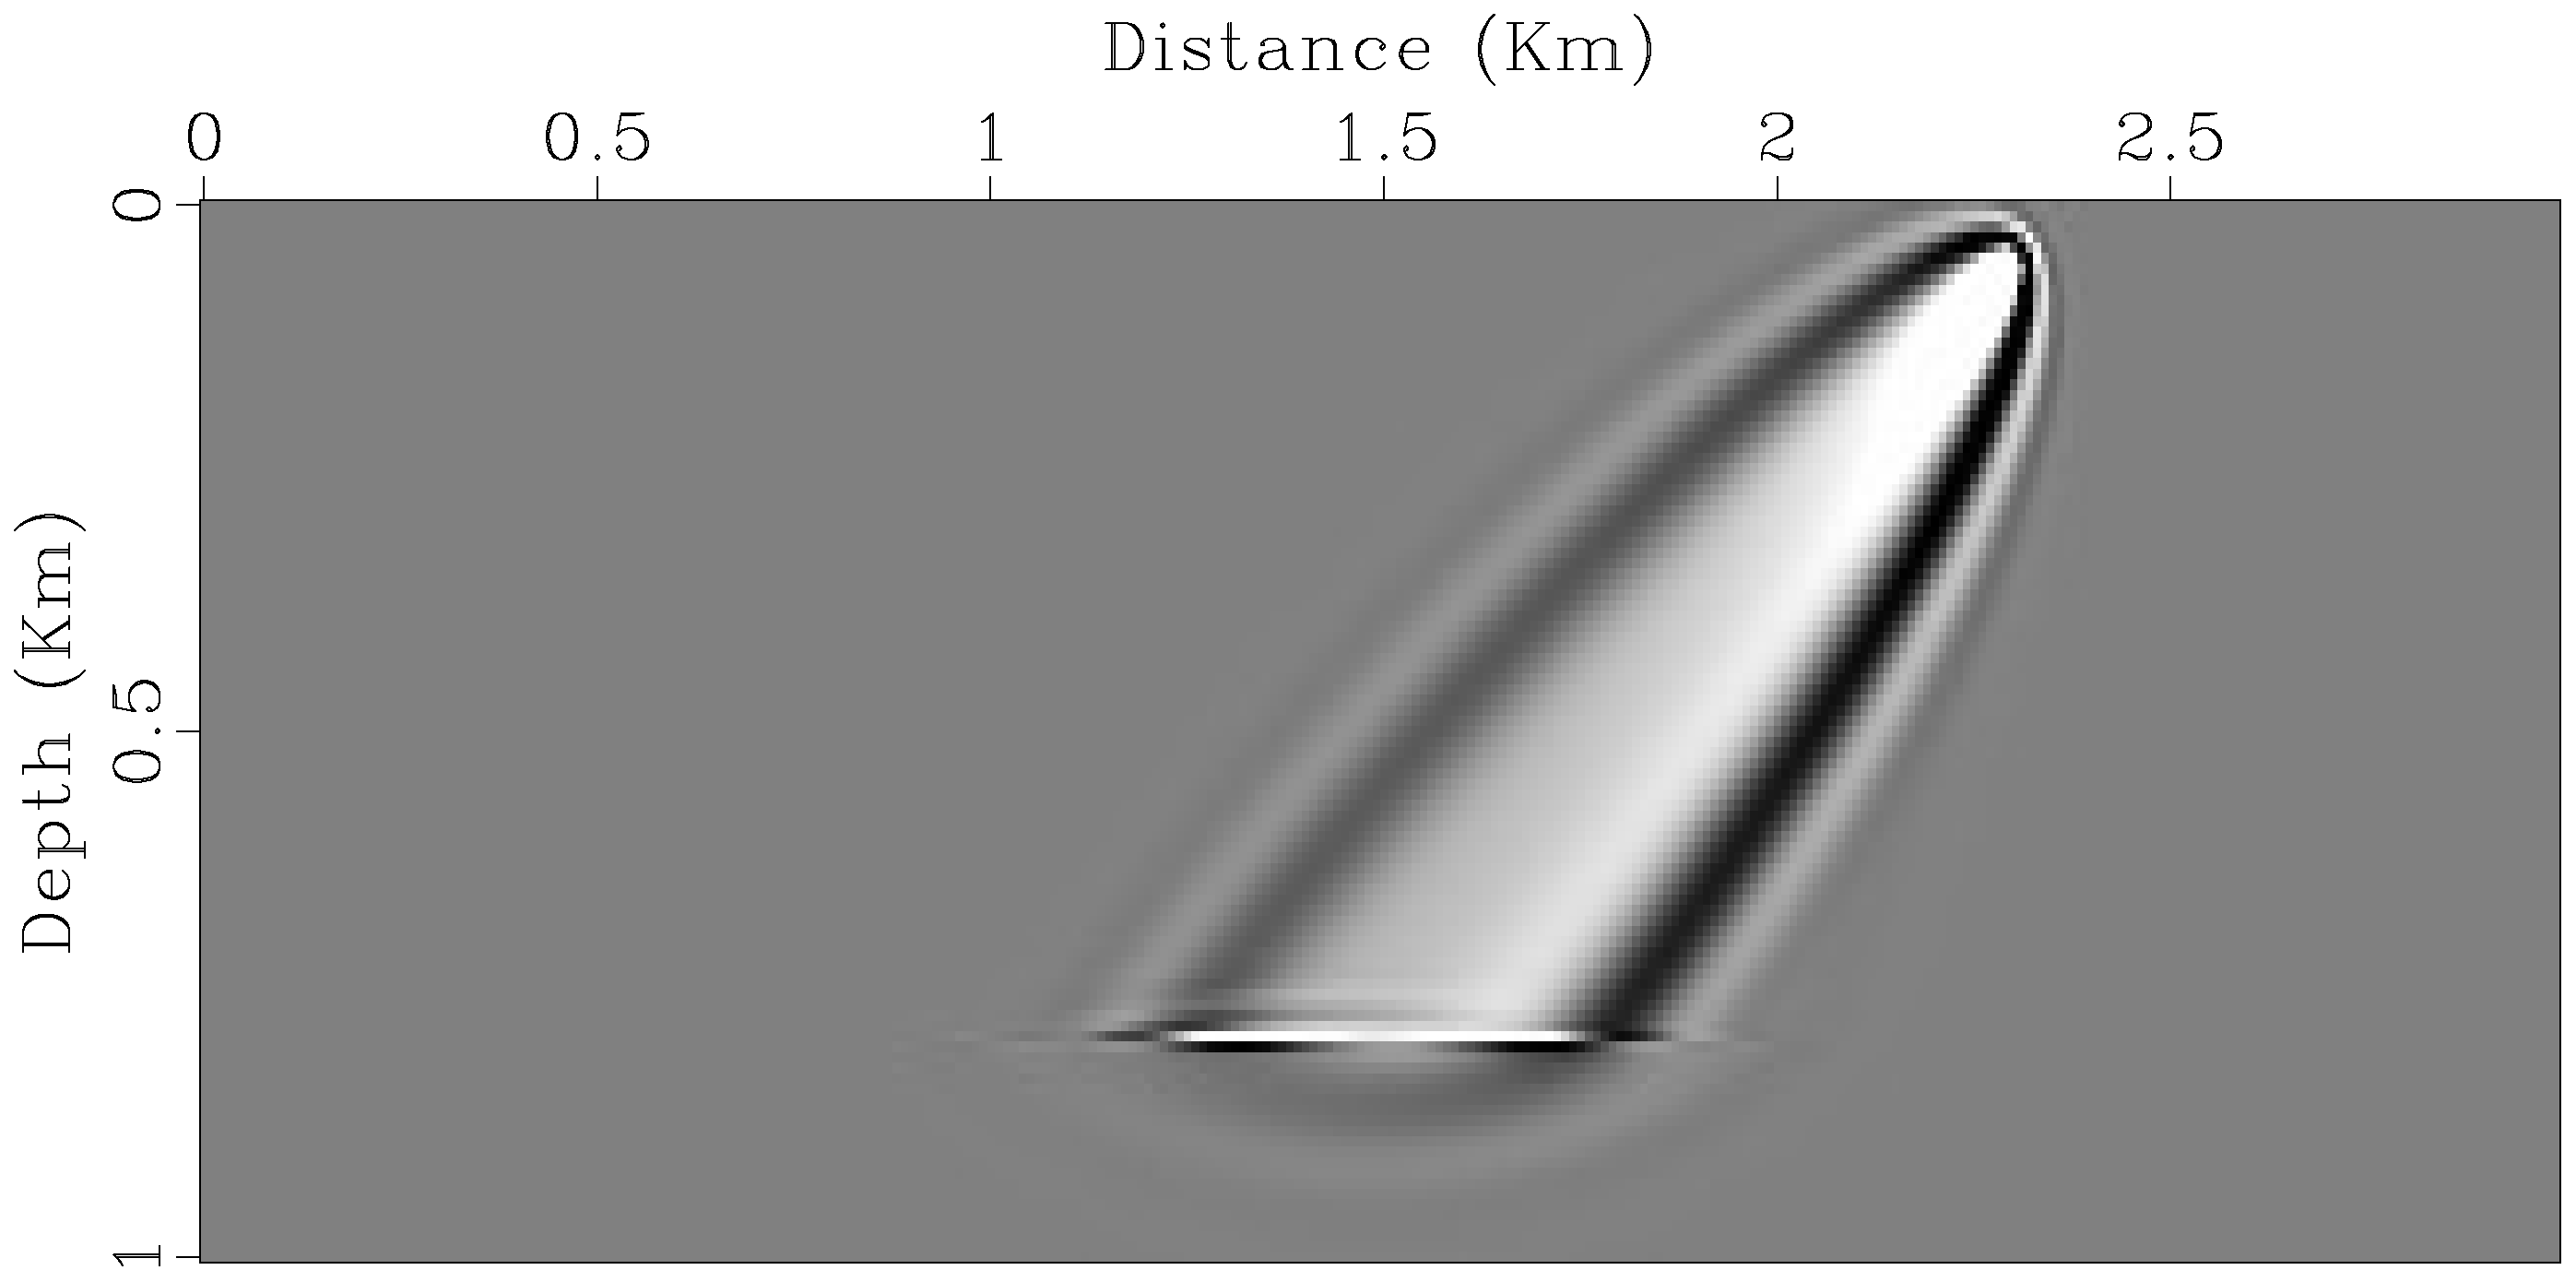
\includegraphics[width=0.45\linewidth]{figure/gradr_rwi_one}}
	\fcaption{常规FWI梯度分解。(a)直达波梯度;(b)偏移响应;(c)源端反射波梯度;
	(d)检波点端反射波梯度。}{The sub-gradients of FWI. (a) direct wave gradient; 
	(b) migration-ellipse; (c) source side gradient; (d) receiver side gradient.
	 }[常规FWI梯度分解]
	\label{fig:grad}
\end{figure*}

RWI主要是通过上下行波分离来提取反射波在反射波路径上的梯度。目前在RWI中用于上下行波分离
的方法主要两种,一种是在光滑的背景模型中加入参数扰动,用Born正演来获取上行的反射波
(\citeA{xu:2012a};\citeA{ma.hale:2013};\citeA{chi:2015});另一种是在频率-波数域
用方向分解来区分上下行波(\citeA{wang:2016})。另外,单成波方程自然地考虑了波的传播
方向,非常适合RWI的框架,已逐渐开始被学者用于RWI的研究中(\citeA{dong:2018})。
本节将用基于Born正演的方式来重述RWI的推导。

根据\citeB{ma.hale:2013}的推导,将模型参数$\mathbf{m}$分解为光滑的低波数背景模型
$\mathbf{m}^s$和高波数扰动$\mathbf{m}^r$(图~\ref{fig:schematic_rwi}):
\begin{equation}
	\mathbf{m}=\mathbf{m}^s+\mathbf{m}^r.
\end{equation}
其中光滑的背景参数$\mathbf{m}^s$控制波传播的运动学信息,即背景波场$\mathbf{p}_b
\equiv p_b(\mathbf{x}_s,\mathbf{x}_g,t)$:
\begin{equation}
	\left(\mathbf{m}^s\frac{\partial^2}{\partial t^2}-\bigtriangledown^2\right)\mathbf{p}_b
	=f(t,\mathbf{x}_s),
\end{equation}
高波数扰动$\mathbf{m}^r$对应于反射波场$\mathbf{p}_c\equiv p_c(\mathbf{x}_s,\mathbf{x}_g,t)$:
\begin{equation}
	\left((\mathbf{m}^s+\mathbf{m}^r)\frac{\partial^2}{\partial t^2}-\bigtriangledown^2\right)
	\mathbf{p}_c=-\mathbf{m}^r\frac{\partial^2}{\partial t^2}\mathbf{p}_b,
\end{equation}
式中$\mathbf{m}^r$和$\mathbf{m}^s$是慢度的平方,$f(t,\mathbf{x}_s)$表示震源子波。

\begin{figure*}[!htbp]
	\centering
	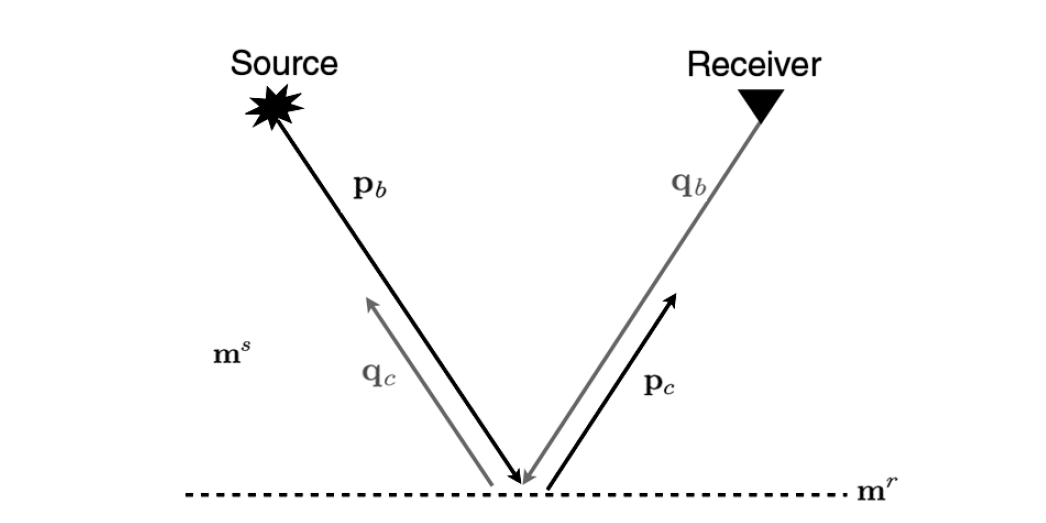
\includegraphics[width=0.7\linewidth]{figure/schematic_rwi}
	\fcaption{RWI波场分解及波路径示意图,参数的高波数成分($\mathbf{m}^r$)扰动背景场
	$\mathbf{p}_b$和$\mathbf{q}_b$产生背向散射场$\mathbf{p}_c$和$\mathbf{q}_c$,可以看作
	是”透射波“从震源出发沿波路径到达反射位置$\mathbf{m}^r$然后再返回接收点。}
	{Schematic of RWI. The high-wavenumber component
	$m^r$ perturbs wavefields $\mathbf{p}_b$ and $\mathbf{q}_b$ in the
	low-wavenumber background $m^s$ and contributes to back-scattering
	wavefields $\mathbf{p}_c$ and $\mathbf{q}_c$, which can be considered
	“transmission” waves propagating along the wave paths between $m^r$ and
	the source and receiver.}[RWI波场分解及波路径示意图]
	\label{fig:schematic_rwi}
\end{figure*}

根据伴随状态法(\citeA{plessix:2006}),低波数背景模型的梯度可以表示为(\citeA{ma.hale:2013}):
\begin{equation}
	\partial_{\mathbf{m}^s}\mathcal{J}=-\int d\mathbf{x}_sdt\mathbf{q}_c\ddot{\mathbf{p}}_b
	-\int d\mathbf{x}_sdt\mathbf{q}_b\ddot{\mathbf{p}}_c,
	\label{eq:grad_ms}
\end{equation}
高波数的扰动模型的梯度为:
\begin{equation}
	\partial_{\mathbf{m}^r}\mathcal{J}=-\int d\mathbf{x}_sdt\mathbf{q}_b\ddot{\mathbf{p}}_b
\end{equation}
式中$\mathbf{q}_b\equiv q_b(\mathbf{x}_s,\mathbf{x}_g,t)$和
$\mathbf{q}_c\equiv q_c(\mathbf{x}_s,\mathbf{x}_g,t)$是伴随场,即伴随方程的解。
方程~\ref{eq:grad_ms}右端的第一项表示源端的正传波场$\ddot{\mathbf{p}}_b$与反传波场
$\mathbf{q}_c$的零延迟互相关(图~\ref{fig:grad}c),同样地,第二项是正传波场$\ddot{\mathbf{p}}_c$和检波点端
反传波场$\mathbf{q}_b$的零延迟互相关(图~\ref{fig:grad}d)。正如图~\ref{fig:schematic_rwi}所示,模型的高波数
成分$\mathbf{m}^r$散射源端的正传背景场$\mathbf{p}_b$和检波点端的反传背景场$\mathbf{q}_b$,
换句话说,$\mathbf{m}^r$中的每一点都可以看成是虚拟震源来产生散射波场$\mathbf{p}_c$和
$\mathbf{q}_c$。背景模型的梯度$\partial_{\mathbf{m}^s}\mathcal{J}$跟预想的一样,是沿反射波的波路径分布的,
即从震源出发到达地下反射位置然后再返回接收点。这样的梯度携带了地下中深层的参数信息,用以更新中深层的背景
模型是可靠的。相反,$\partial_{\mathbf{m}^r}\mathcal{J}$类似于RTM成像结果,主要分布在反射
位置$\mathbf{m}^r$附近,用以产生反射数据。

\newpage
\subsection{基于粘声方程的反射全波形反演}
\vspace{-1.0cm}
根据第二章第二节的推导,对于给定的速度以及$Q$模型,压力波场可用如下SLS方程进行计算:
     \begin{eqnarray}
        \begin{aligned}
        \frac{\partial P}{\partial t} -
        K(\tau+1)(\frac{\partial v_x}{\partial x}
        +\frac{\partial v_z}{\partial z})-r_p &=f(\mathbf{x}_s,t),
        \\
        \frac{\partial v_x}{\partial t} - \frac{1}{\rho}\frac{\partial P}{\partial x}
        &=0,\\
        \frac{\partial v_z}{\partial t} - \frac{1}{\rho}\frac{\partial P}{\partial z}&=0,\\
        \frac{\partial{r_p}}{\partial t} +
        \frac{1}{\tau_\sigma}\left[r_p+K\tau(\frac{\partial
        v_x}{\partial x}+\frac{\partial v_z}{\partial z})\right]&=0,
        \end{aligned}
        \label{eq:viscoacoustic}
    \end{eqnarray}
式中$v_x$和$v_z$表示质点的振动速度,$P$表示压力场,$r_p$为记忆变量,$K$表示介质的体积
模量,为了简化表示我们假定密度是常数。应力以及应变的驰豫参数$\tau_\sigma$,$\tau_\epsilon$
以及$\tau$与品质因子$Q$和参考频率$f_\omega$有关,在地震勘探应用中,通常选取震源子波
的中心频率为其参考频率,即有:
    \begin{eqnarray}
        \begin{aligned}
            \tau_\sigma &= \frac{\sqrt{1+\frac{1}{Q^2}}-\frac{1}{Q}}{f_\omega},\\
            \tau_\epsilon &= \frac{1}{f^2_\omega\tau_\sigma}=\frac{\sqrt{1+\frac{1}{Q^2}}+\frac{1}{Q}}{f_\omega},
        \end{aligned}
    \end{eqnarray}
以及
    \begin{eqnarray}
        \tau=\frac{\tau_\epsilon}{\tau_\sigma}-1=\frac{2}{Q}(\frac{1}{Q}+\sqrt{1+\frac{1}{Q^2}}).
        \label{eq:tq}
    \end{eqnarray}

在$Q$-RWI中,主要反演背景的$Q$,我们认为衰减对宏观地震波的影响主要发生在波路径上,
即是一种传播效应不是界面效应,所以不对$Q$进行波数成分的分解。为了描述波路径产生反射波,携带
衰减信息,我们将体积模量$K$分解为光滑背景$K_0$和高波数扰动$\delta K$:
\begin{equation}
	K = K_0 + \delta K.
\end{equation}
根据SLS粘声波方程~\ref{eq:viscoacoustic}以及Born近似假设,$Q$-RWI的物理状态方程可
写为如下矩阵向量乘的形式:
\begin{equation}
    \mathbf{L}\mathbf{w} = \mathbf{f},
    \label{eq:state}
\end{equation}
其中
    \begin{eqnarray*}
        \mathbf{L}= 
        \begin{bmatrix}
            \begin{smallmatrix}
            \frac{\partial}{\partial t} &-K_0(\tau +1)\frac{\partial}{\partial x}
            &-K_0(\tau +1)\frac{\partial}{\partial z} &-1 &0 &0 &0 &0\cr
            -\frac{1}{\rho}\frac{\partial}{\partial x} &\frac{\partial}{\partial t} &0
            &0 &0 &0 &0 &0\cr
            -\frac{1}{\rho}\frac{\partial}{\partial z} &0 &\frac{\partial}{\partial t}
            &0 &0 &0 &0 &0\cr
            0 & \frac{\tau}{\tau_\sigma}K_0\frac{\partial}{\partial x}
            &\frac{\tau}{\tau_\sigma}K_0\frac{\partial}{\partial z}
            &\frac{\partial}{\partial t}+\frac{1}{\tau_\sigma} &0 &0 &0 &0 \cr
            0 &-\delta K(\tau+1)\frac{\partial}{\partial x} &-\delta
            K(\tau+1)\frac{\partial}{\partial z} &0 &\frac{\partial}{\partial t}
            &-K_0(\tau +1)\frac{\partial}{\partial x} &-K_0(\tau
            +1)\frac{\partial}{\partial z} &-1 \cr
            0 &0 &0 &0 &-\frac{1}{\rho}\frac{\partial}{\partial x}
            &\frac{\partial}{\partial t} &0 &0\cr
            0 &0 &0 &0 &-\frac{1}{\rho}\frac{\partial}{\partial z} &0
            &\frac{\partial}{\partial t} &0\cr
            0 &\frac{\tau}{\tau_\sigma}\delta K\frac{\partial}{\partial x}
            &\frac{\tau}{\tau_\sigma}\delta K\frac{\partial}{\partial z} &0 &0 
            & \frac{\tau}{\tau_\sigma}K_0\frac{\partial}{\partial x}
            &\frac{\tau}{\tau_\sigma}K_0\frac{\partial}{\partial z}
            &\frac{\partial}{\partial t}+\frac{1}{\tau_\sigma}
            \end{smallmatrix}
        \end{bmatrix}
    \end{eqnarray*}
以及
    \begin{eqnarray*}
        \mathbf{w} = 
        \begin{bmatrix}
            P \cr v_x \cr v_z \cr r_p \cr\delta P \cr\delta v_x \cr\delta v_z
            \cr\delta r_p
        \end{bmatrix},
        \mathbf{f} = 
        \begin{bmatrix}
            f \cr 0\cr 0\cr 0 \cr 0\cr 0 \cr 0\cr 0
        \end{bmatrix}.
    \end{eqnarray*}
$\mathbf{w}$表示状态变量,$\mathbf{L}$表示正演模拟算子。在这种情况下,
正算子的伴随算子$\mathbf{L}^\ast$有如下表达式:
    \begin{eqnarray}
        \mathbf{L}^\ast =  
        \begin{bmatrix}
            \begin{smallmatrix}
            -\frac{\partial}{\partial t} &\frac{\partial}{\partial x}\frac{1}{\rho}
            &\frac{\partial}{\partial z}\frac{1}{\rho} &0 &0 &0 &0 &0\cr
            \frac{\partial}{\partial x}K_0(\tau +1) &-\frac{\partial}{\partial t} &0 
            &-\frac{\partial}{\partial x}\frac{\tau}{\tau_\sigma}K_0
            &\frac{\partial}{\partial x}\delta K(\tau+1) &0 &0
            &-\frac{\partial}{\partial x}\frac{\tau}{\tau_\sigma}\delta K \cr
            \frac{\partial}{\partial z}K_0(\tau +1) &0 &-\frac{\partial}{\partial t} 
            &-\frac{\partial}{\partial z}\frac{\tau}{\tau_\sigma}K_0
            &\frac{\partial}{\partial z}\delta K(\tau+1) &0 &0
            &-\frac{\partial}{\partial z}\frac{\tau}{\tau_\sigma}\delta K \cr
            -1 &0 &0 &-\frac{\partial}{\partial t}+\frac{1}{\tau_\sigma} &0 &0 &0 &0\cr
            0 &0 &0 &0 &-\frac{\partial}{\partial t} &\frac{\partial}{\partial
            x}\frac{1}{\rho} &\frac{\partial}{\partial z}\frac{1}{\rho} &0\cr
            0 &0 &0 &0 &\frac{\partial}{\partial x}K_0(\tau +1)
            &-\frac{\partial}{\partial t} &0 &-\frac{\partial}{\partial
            x}\frac{\tau}{\tau_\sigma}K_0 \cr
            0 &0 &0 &0 &\frac{\partial}{\partial z}K_0(\tau +1) &0
            &-\frac{\partial}{\partial t} &-\frac{\partial}{\partial
        z}\frac{\tau}{\tau_\sigma}K_0 \cr
           0 &0 &0 &0 &-1 &0 &0 &-\frac{\partial}{\partial t}+\frac{1}{\tau_\sigma}
            \end{smallmatrix}
        \end{bmatrix},
		\label{eq:ad_operator}
    \end{eqnarray}
式中$\ast$表示伴随。对于真实的地质模型,驰豫参数$\tau$比$\tau_\sigma$和$\tau_\epsilon$
有较宽的数值变化范围。因此我们选择$\tau$作为参数化参数,因为其对$Q$的变化更敏感
(\citeA{dutta.schuster:2016})。用伴随状态法可推导出目标函数$\mathcal{J}(\mathbf{m})$
对驰豫参数$\tau$的梯度为:
   \begin{equation}
    \begin{aligned}
        \frac{\partial \mathcal{J}}{\partial \tau} &= -\langle\frac{\partial \mathbf{L}}{\partial\tau}
        \mathbf{w},\tilde{\mathbf{w}} \rangle \\
        &= {K_0(\frac{\partial v_x}{\partial
        x}+\frac{\partial v_z}{\partial
    z})(-\delta\tilde{P}+\frac{1}{\tau_\sigma}\delta\tilde{r}_p)} \\
    &{+K_0(\frac{\partial \delta v_x}{\partial x}+\frac{\partial \delta
        v_z}{\partial z})(-\tilde{P}+\frac{1}{\tau_\sigma}\tilde{r}_p)} \\
        &{+\delta K(\frac{\partial v_x}{\partial x}+\frac{\partial v_z}{\partial
        z})(-\tilde{P}+\frac{1}{\tau_\sigma}\tilde{r}_p)},
    \end{aligned}
    \label{eq:gradient}
    \end{equation}
式中$\tilde{\mathbf{w}}=\lbrack \delta\tilde{P}, \ \delta \tilde{v}_x, \ \delta \tilde{v}_z, \
\delta \tilde{r}_p, \ \tilde{P}, \ \tilde{v}_x, \ \tilde{v}_z, \ \tilde{r}_p\rbrack ^T$是
物理状态变量$\mathbf{w}$的伴随状态变量($T$表示转置),满足如下伴随方程:
\begin{equation}
	\mathbf{L}^\ast\tilde{\mathbf{w}} = \Delta\mathbf{d}.
\end{equation}
在实际勘探中,通常只接收到了波场的压力分量,所以地震数据的残差只有一个分量,即:
\begin{equation}
    \Delta\mathbf{d} = \lbrack 0, \ 0, \ 0, \ 0, \ \Delta d, \ 0, \ 0, \ 0\rbrack^T.
\end{equation}
本章主要是理论的角度来推导$Q$-RWI方法并证明其对反演深层背景衰减模型的有效性,所以我们
假定介质的背景体积模量$K_0$和扰动$\delta K$都是已知的,并且地震数据是无噪的。在这
中假设下选取振幅差作为目标函数(方程~\ref{eq:misfit_function})是可行的,并且伴随方程的
伴随源有最简单的形式即模拟数据与观测数据的残差。

\begin{figure*}[!htbp]
    \centering
    \subfigure[]{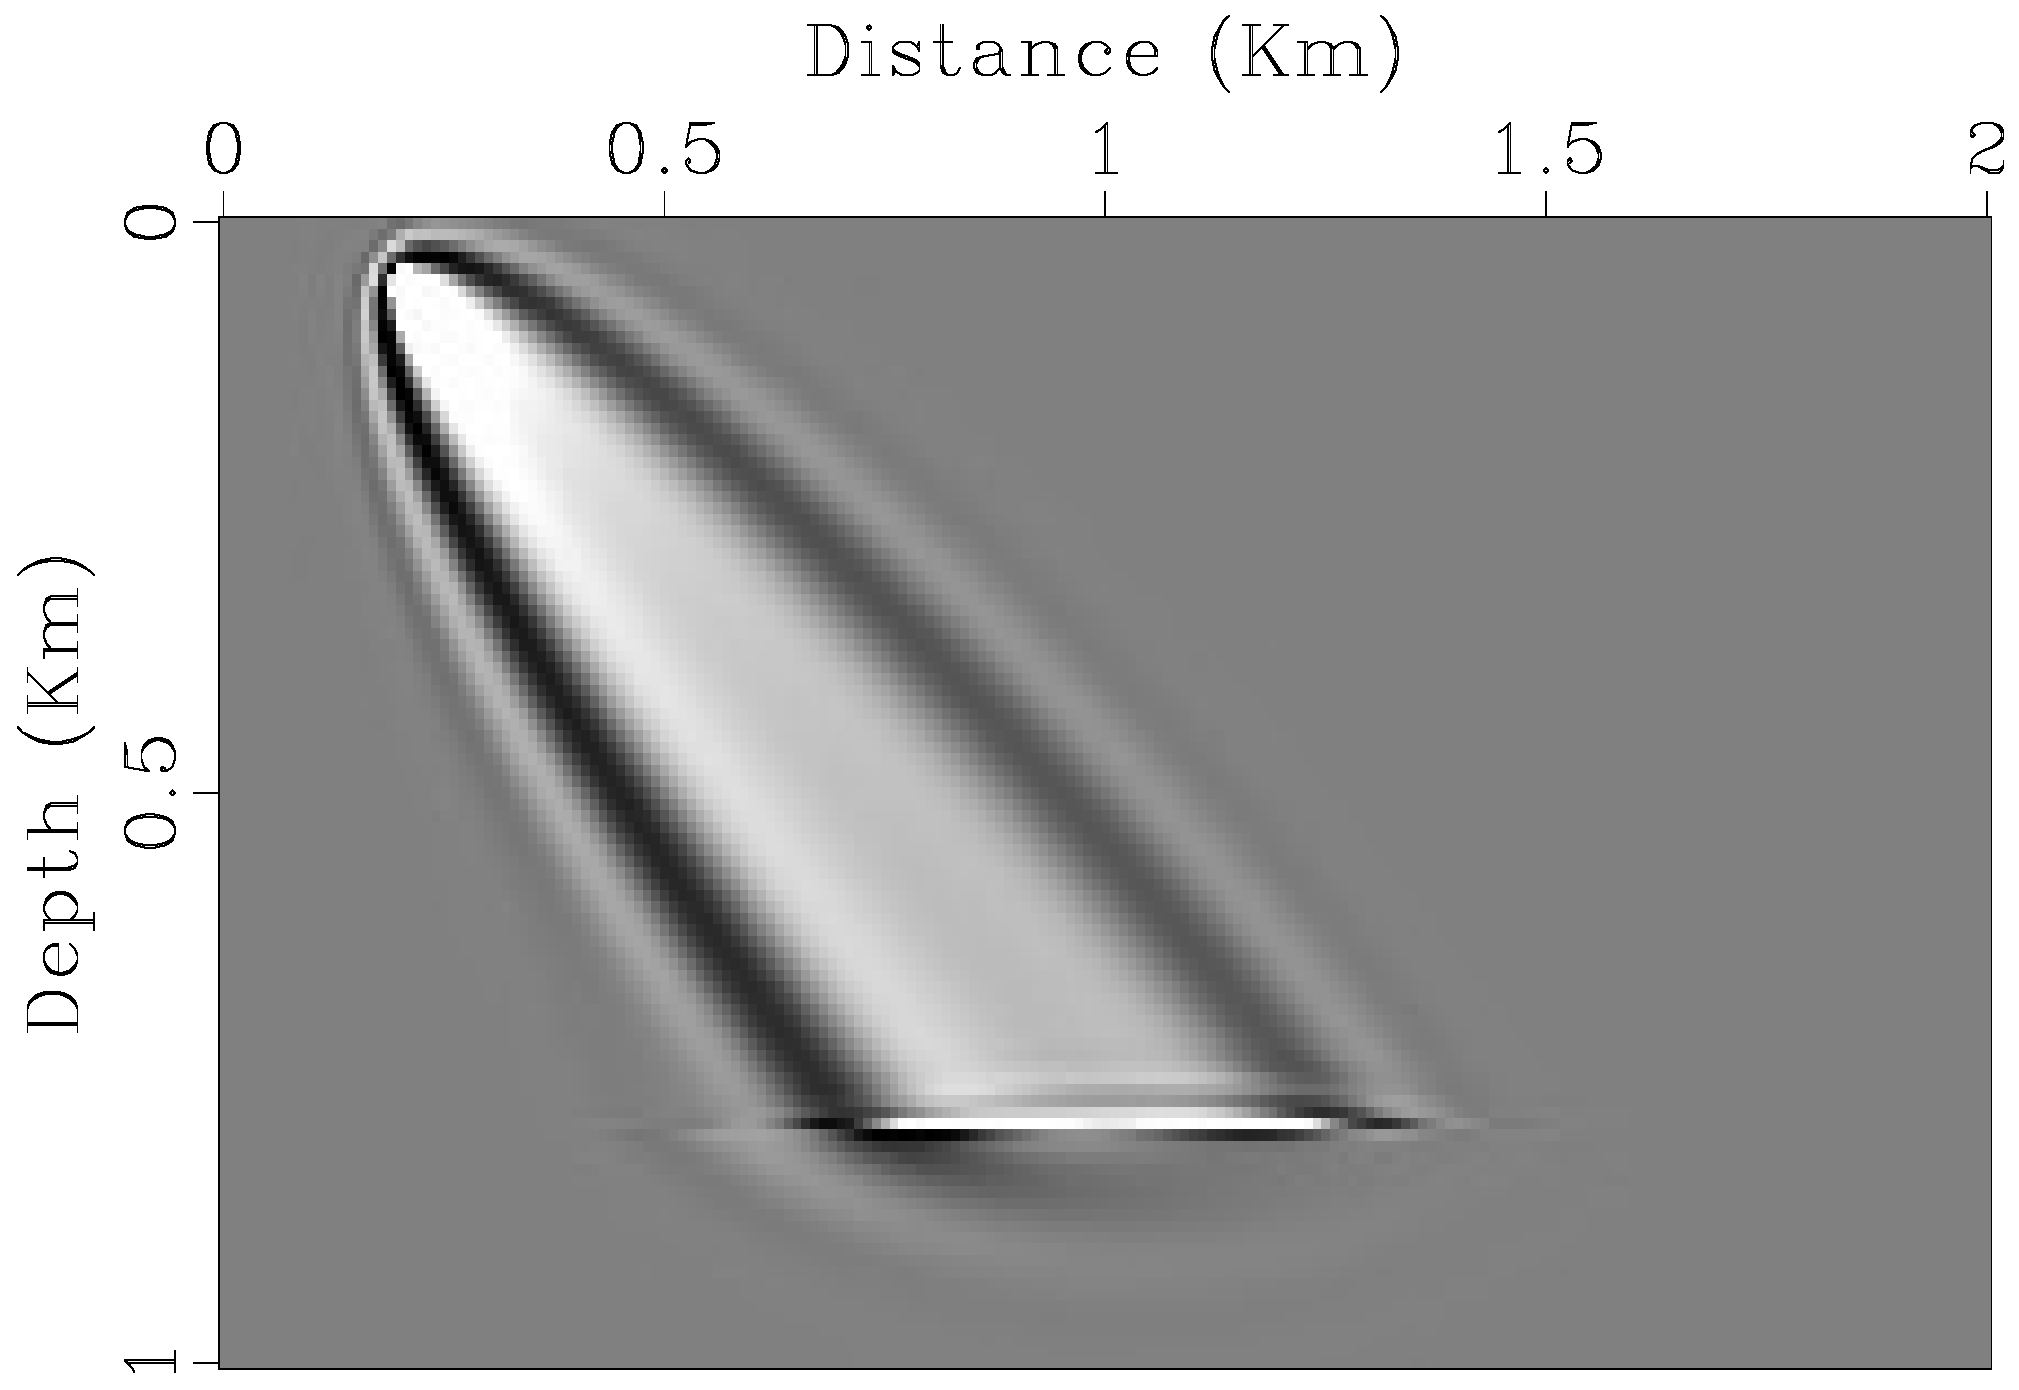
\includegraphics[width=0.49\linewidth]{figure/grad1}}
    \subfigure[]{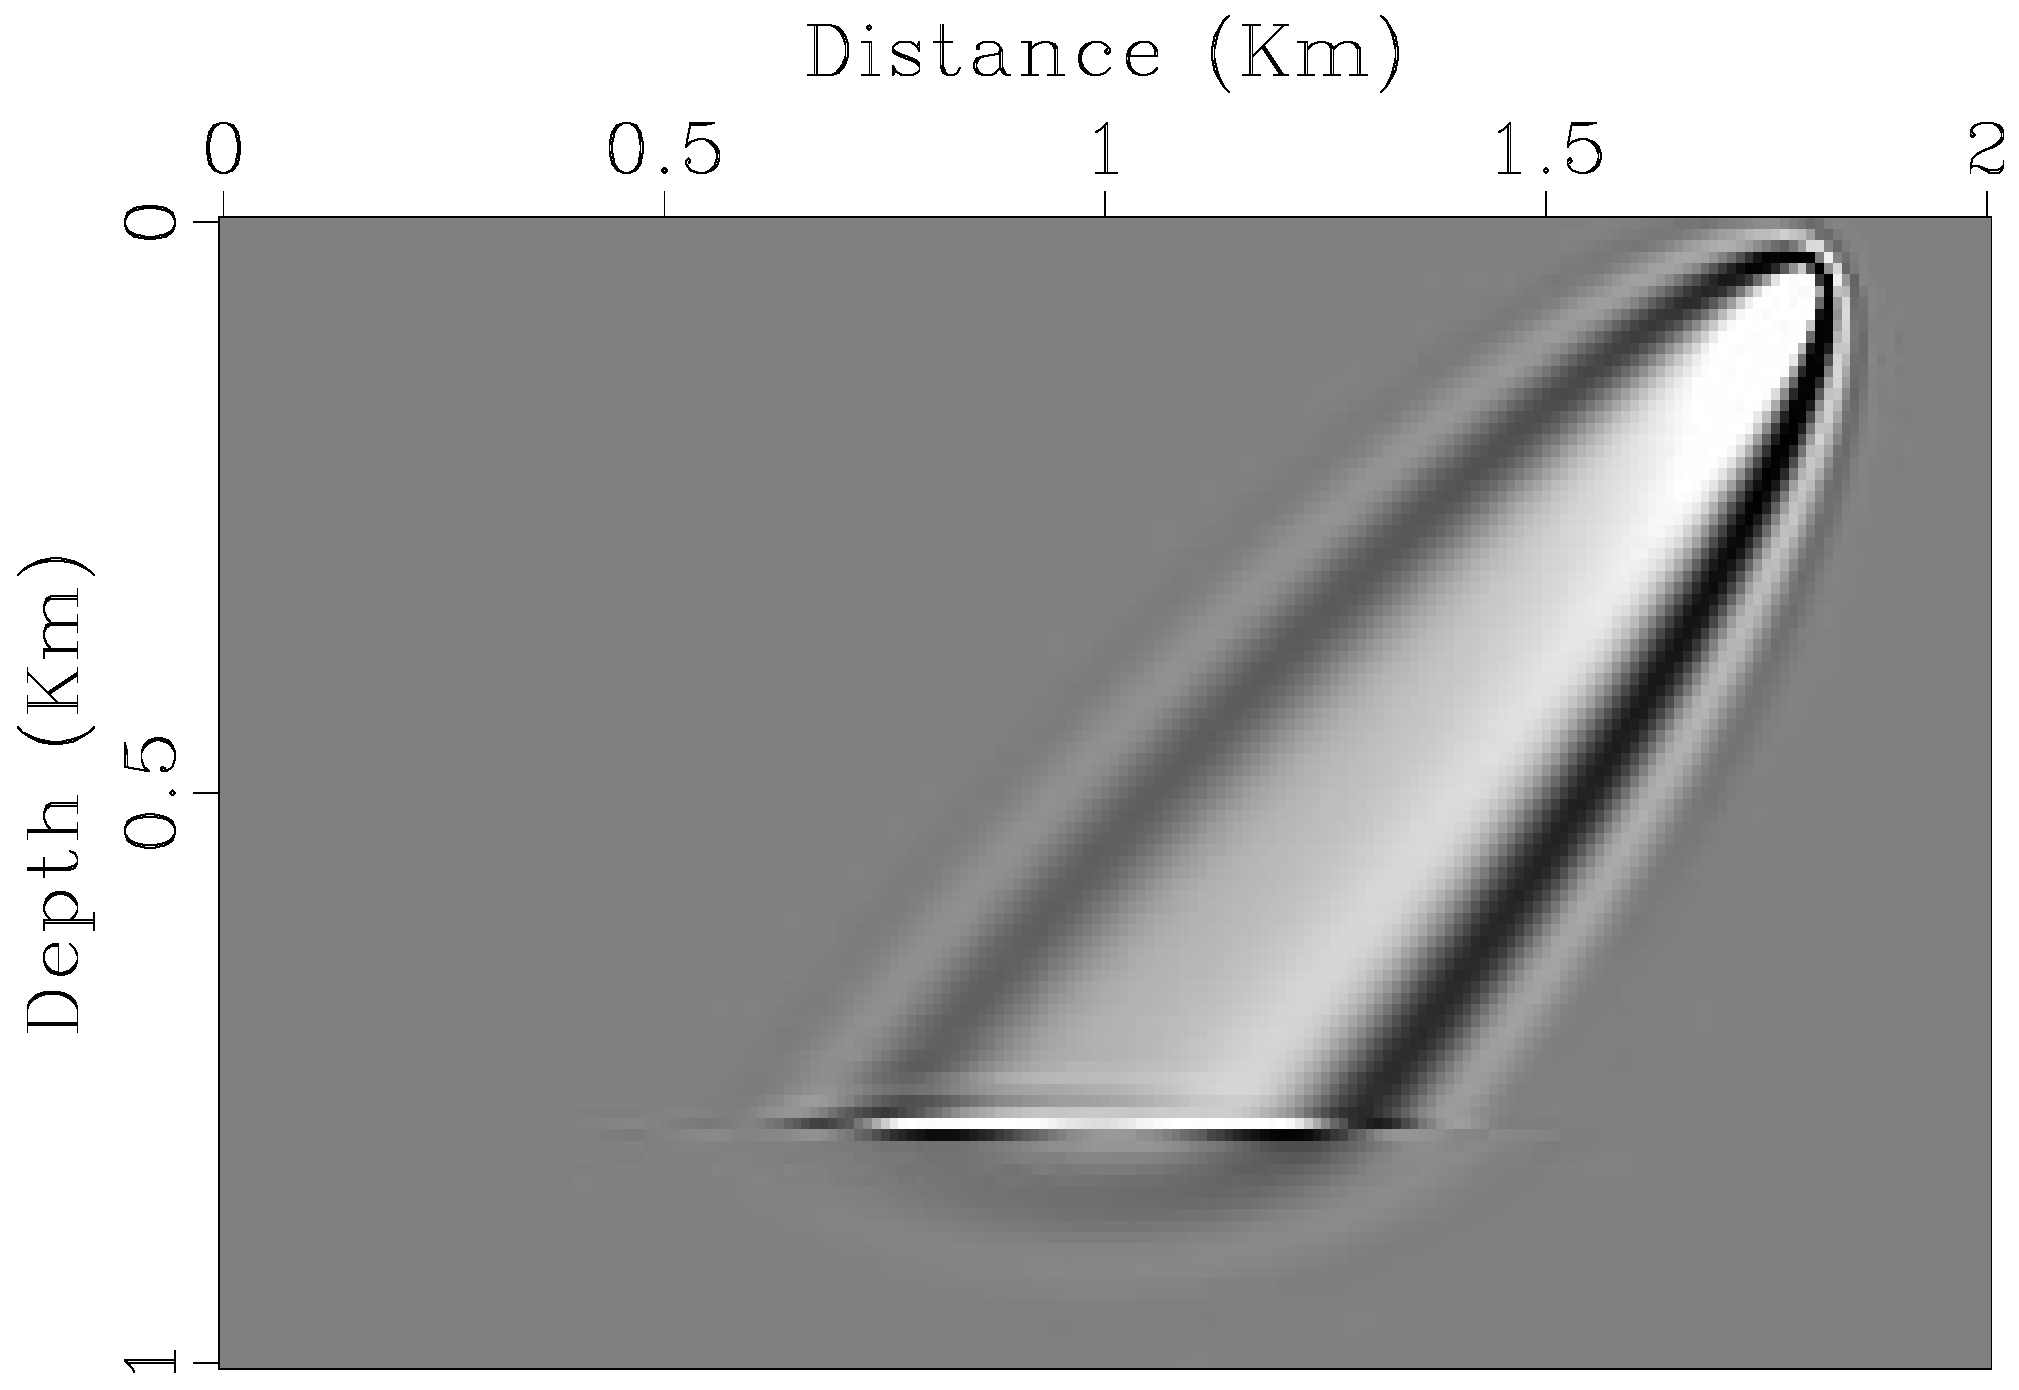
\includegraphics[width=0.49\linewidth]{figure/grad2}}
    \subfigure[]{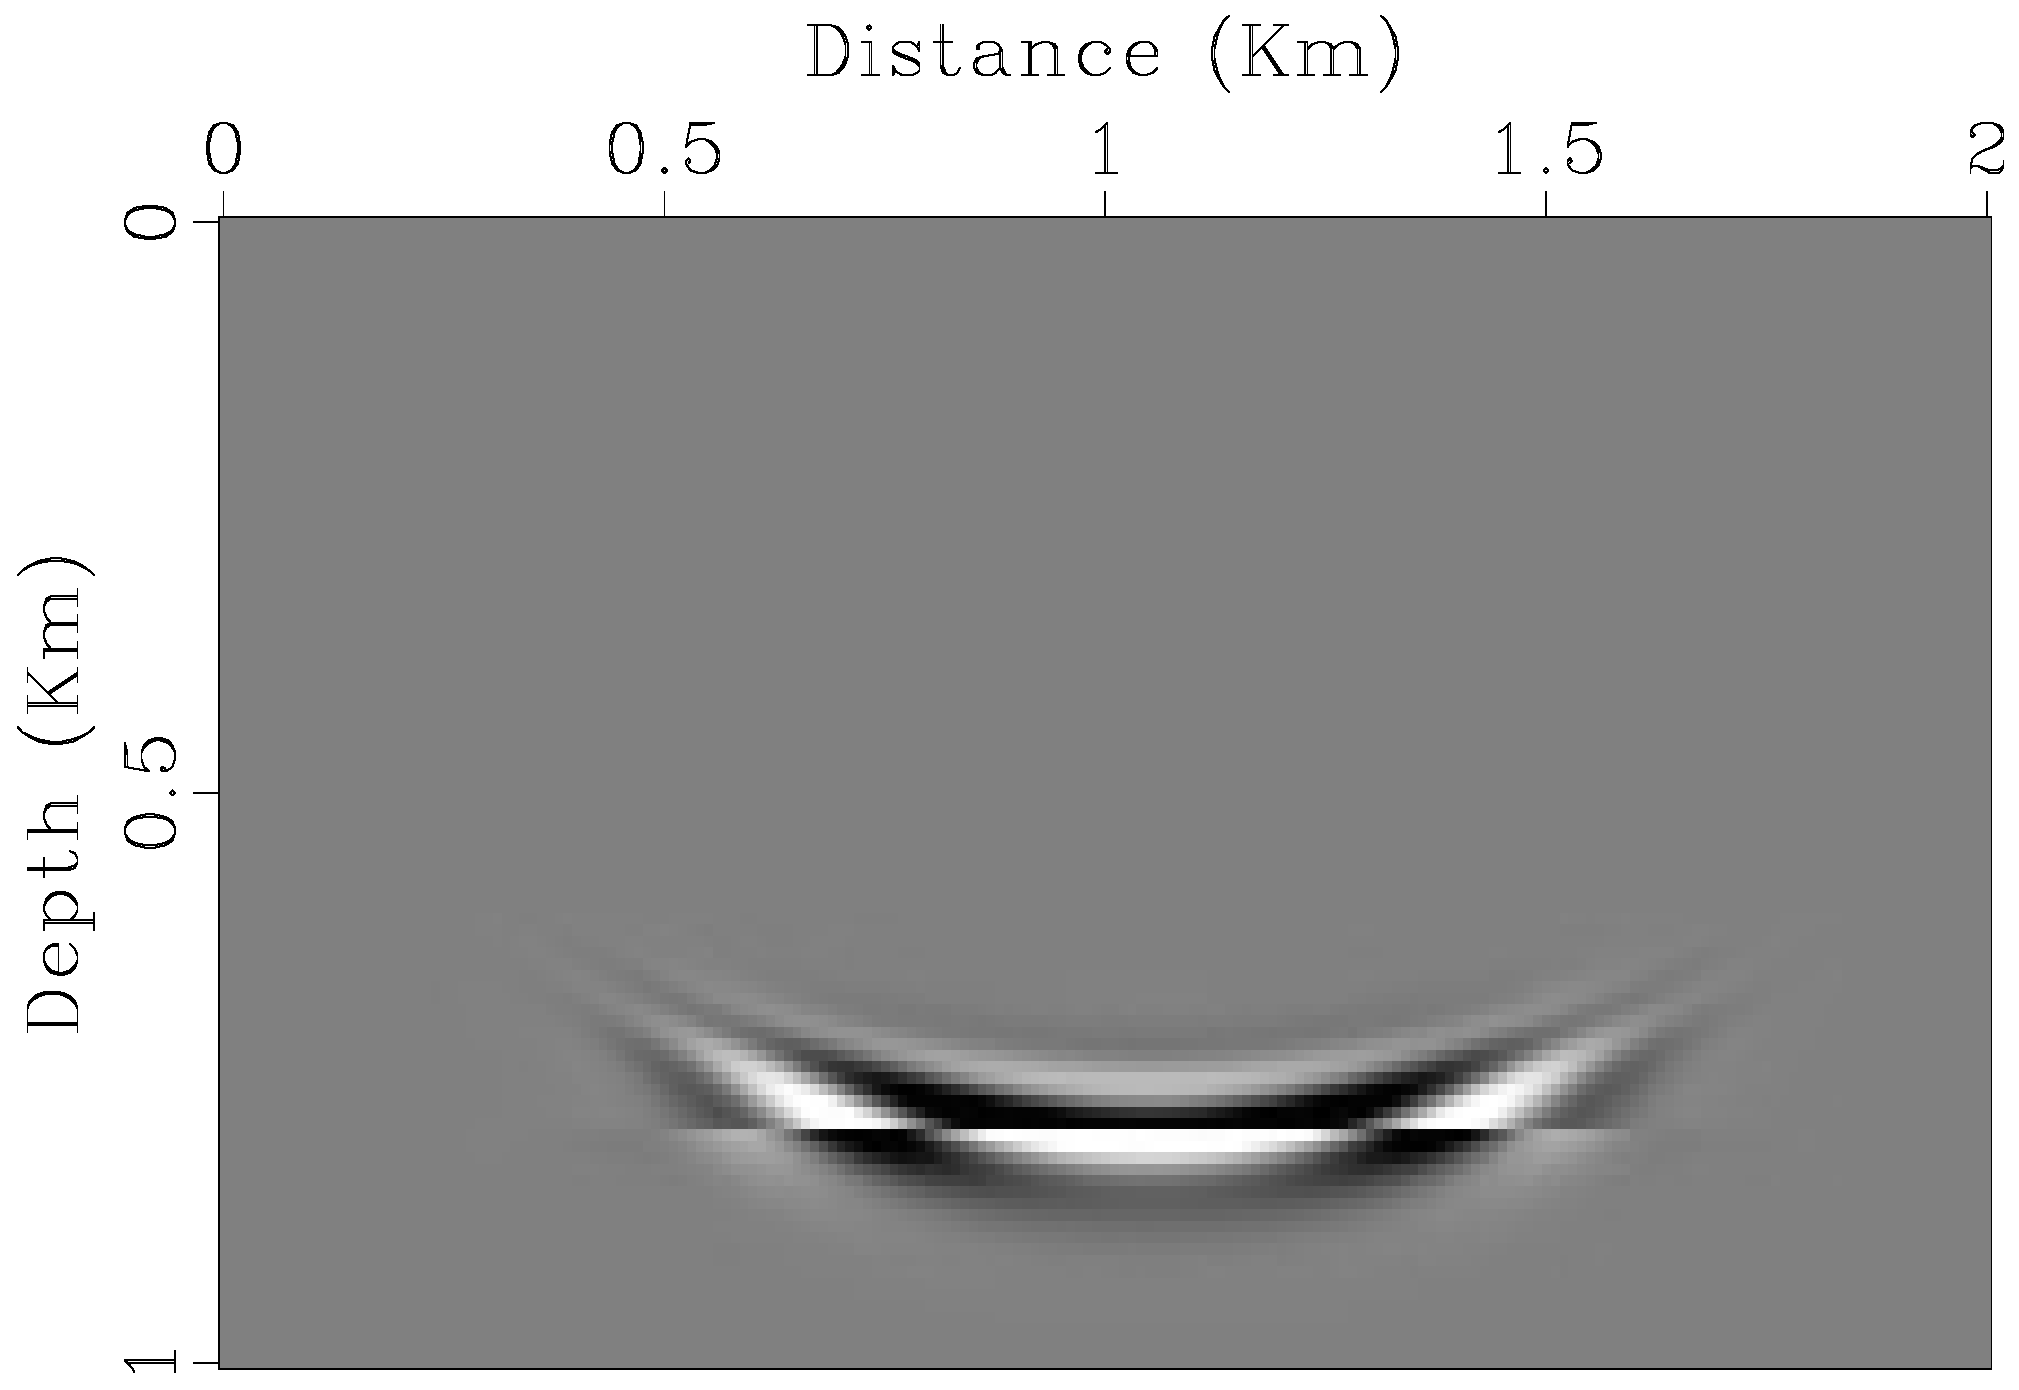
\includegraphics[width=0.49\linewidth]{figure/grad3}}
    \fcaption{两层介质$Q$-RWI中背景$Q$的子梯度。(a)源端梯度;(b)检波点端梯度;
	(c)高波数奇异分量。}{Sub-gradients of $Q$-RWI for simple two-layer model: 
	(a) sourece-side reflection gradient; (b) receiver-side reflection gradient; 
	and singular component.}[两层介质$Q$-RWI中背景$Q$的子梯度]
    \label{fig:grad_qrwi}
\end{figure*}

$Q$-RWI的梯度公式(\ref{eq:gradient})共包含三项。如图~\ref{fig:grad_qrwi}所示,
第一二项”兔耳朵“状的梯度,提供了沿反射波路径的低波数的背景$Q$的更新量。第三项对应于
反射波在成像点的成像结果,对RWI来说是奇异的非光滑的分量。第三项会在反射界面位置更新
高波数成分从而增加反演的非线性程度。在声波的RWI中,\citeB{wu.alkhalifah:2015}观察到
第三项在反射界面处的值的符号与第一二项在反射界面处的值相反,但是数值不一样。他们将
将第三项加入反演中,通过求解一个内部优化问题,用第三项来减弱第一二项在反射界面处
的影响以降低反演的非线性程度。为了不增加反演的计算量,在$Q$-RWI中我们省略掉第三项,
同时用Poynting矢量来简单区分上下行波(\citeA{yoon.marfurt:2006}),
以减弱梯度在反射界面处的奇异性。由图~\ref{fig:grad_poynting}可以看出,无论是单炮单道、
单炮多道还是多炮多道叠加,用Poynting矢量来进行上下行波分离的预条件都减弱了$Q$-RWI中
梯度在反射界面处的奇异性,从而增强了反演的稳定性。以上的$Q$-RWI梯度是基于SLS粘声方程
推导的,这套推导方法同样适合于常$Q$粘声方程,其具体推导可参见附录\ref{chp:dcq}。

\newpage
\begin{figure*}[!htbp]
    \centering
    \subfigure[]{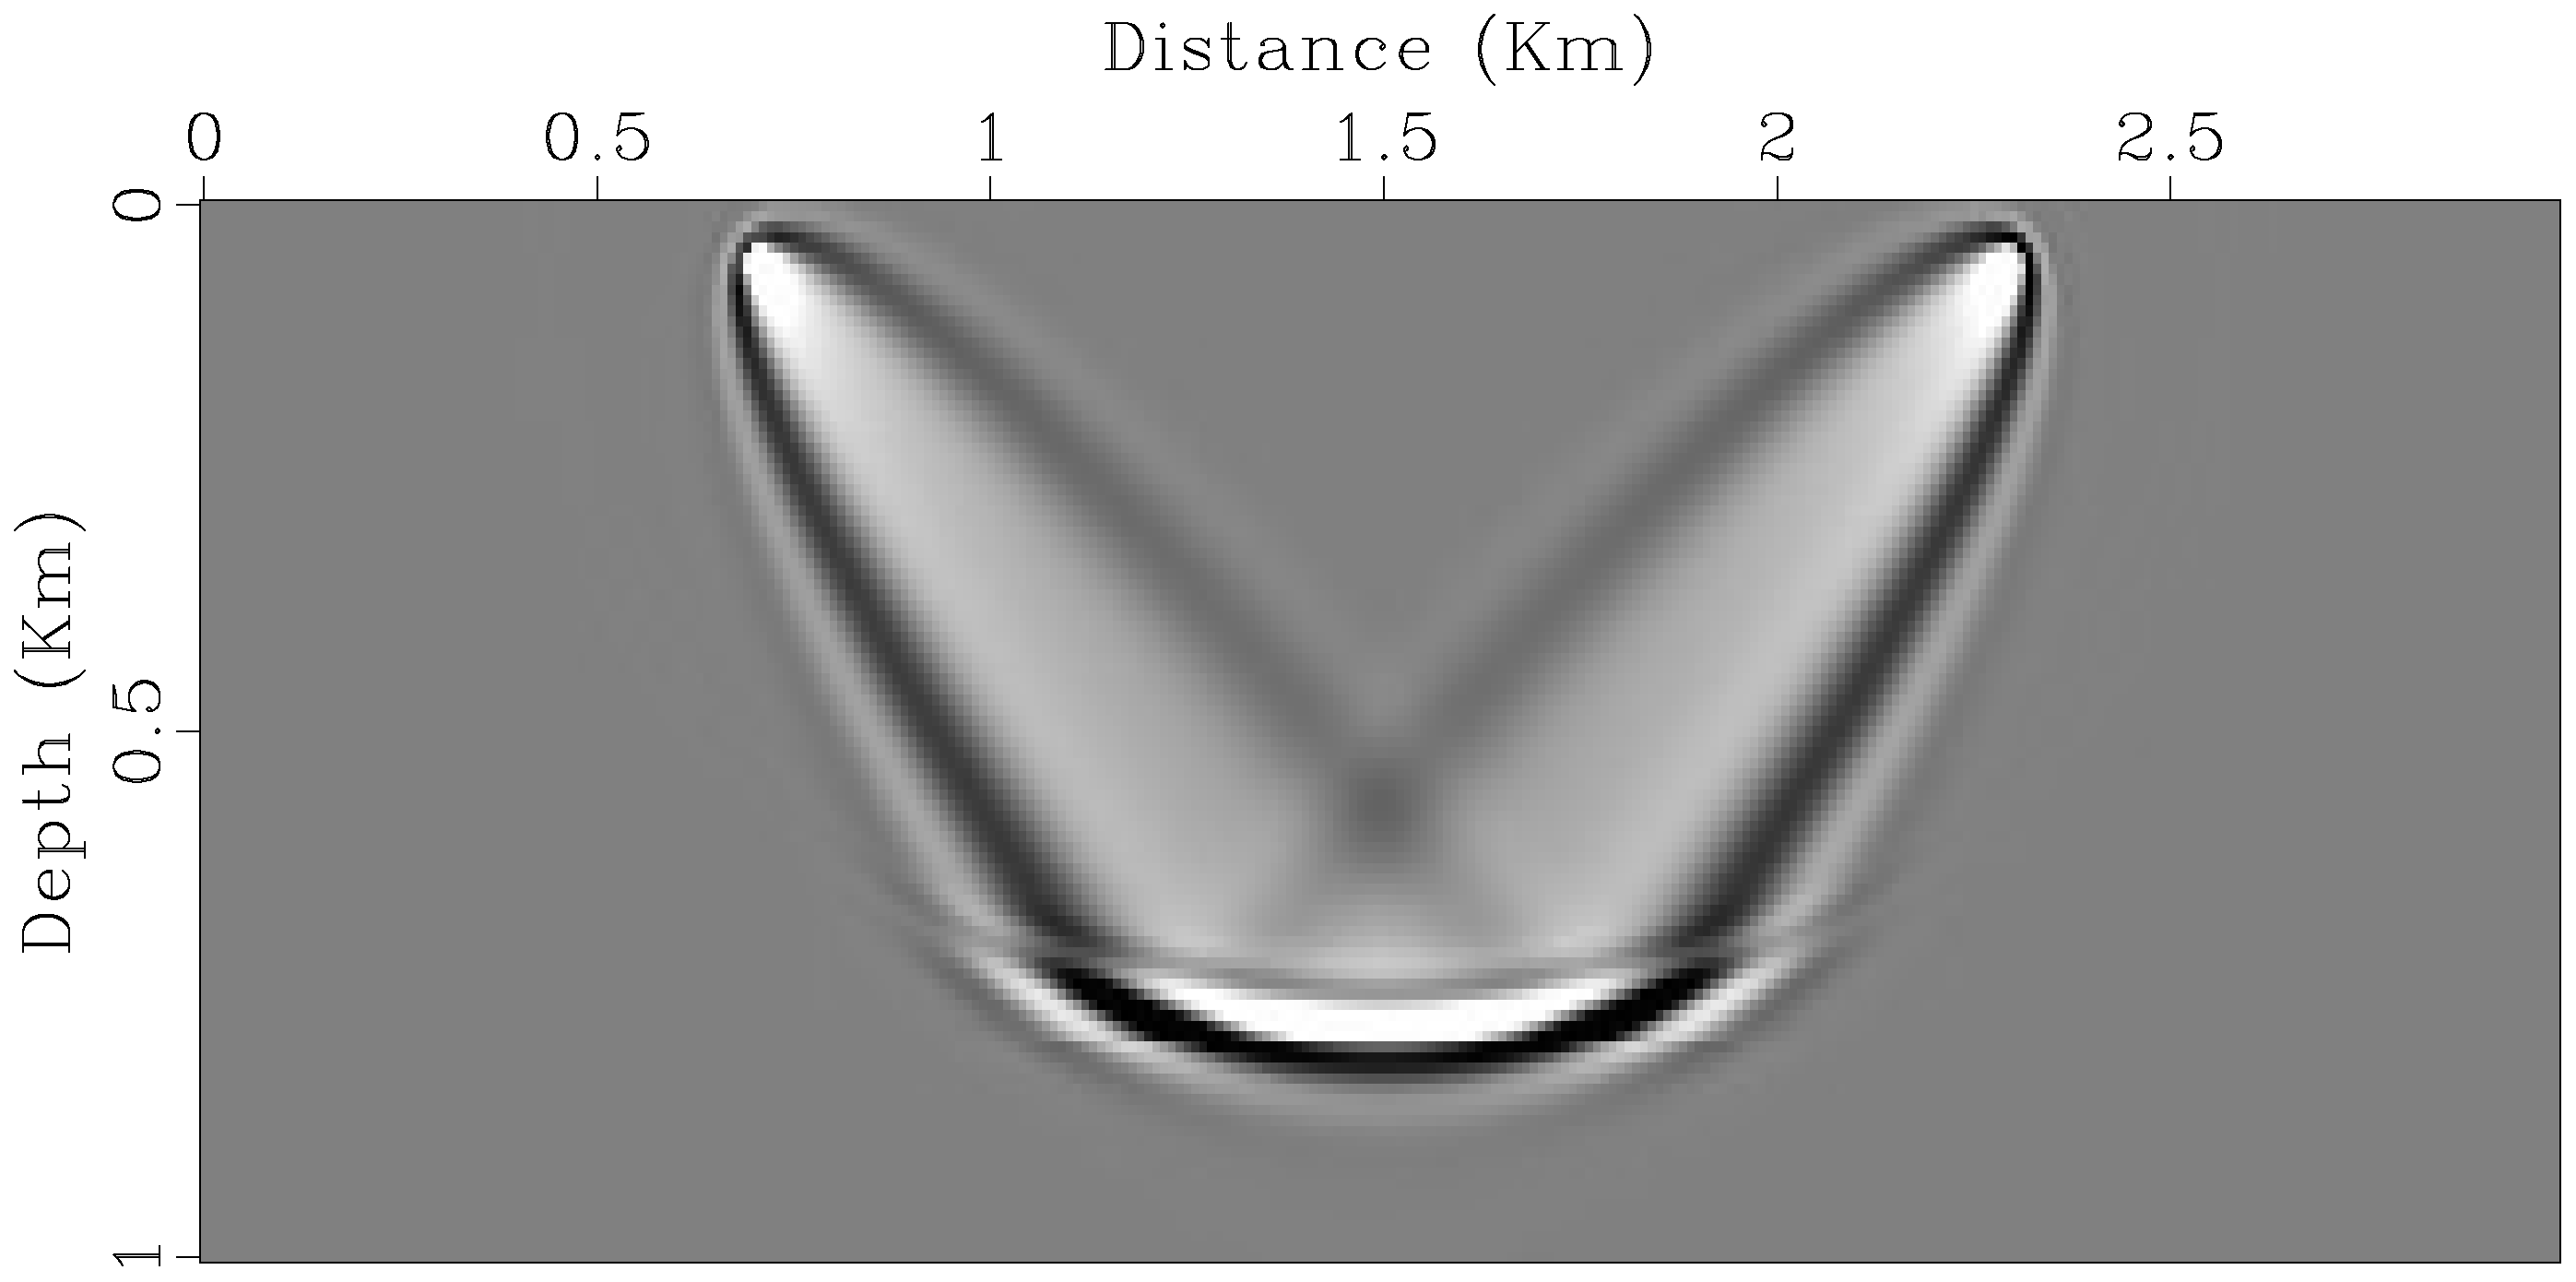
\includegraphics[width=0.49\linewidth]{figure/grad_rwi}}
    \subfigure[]{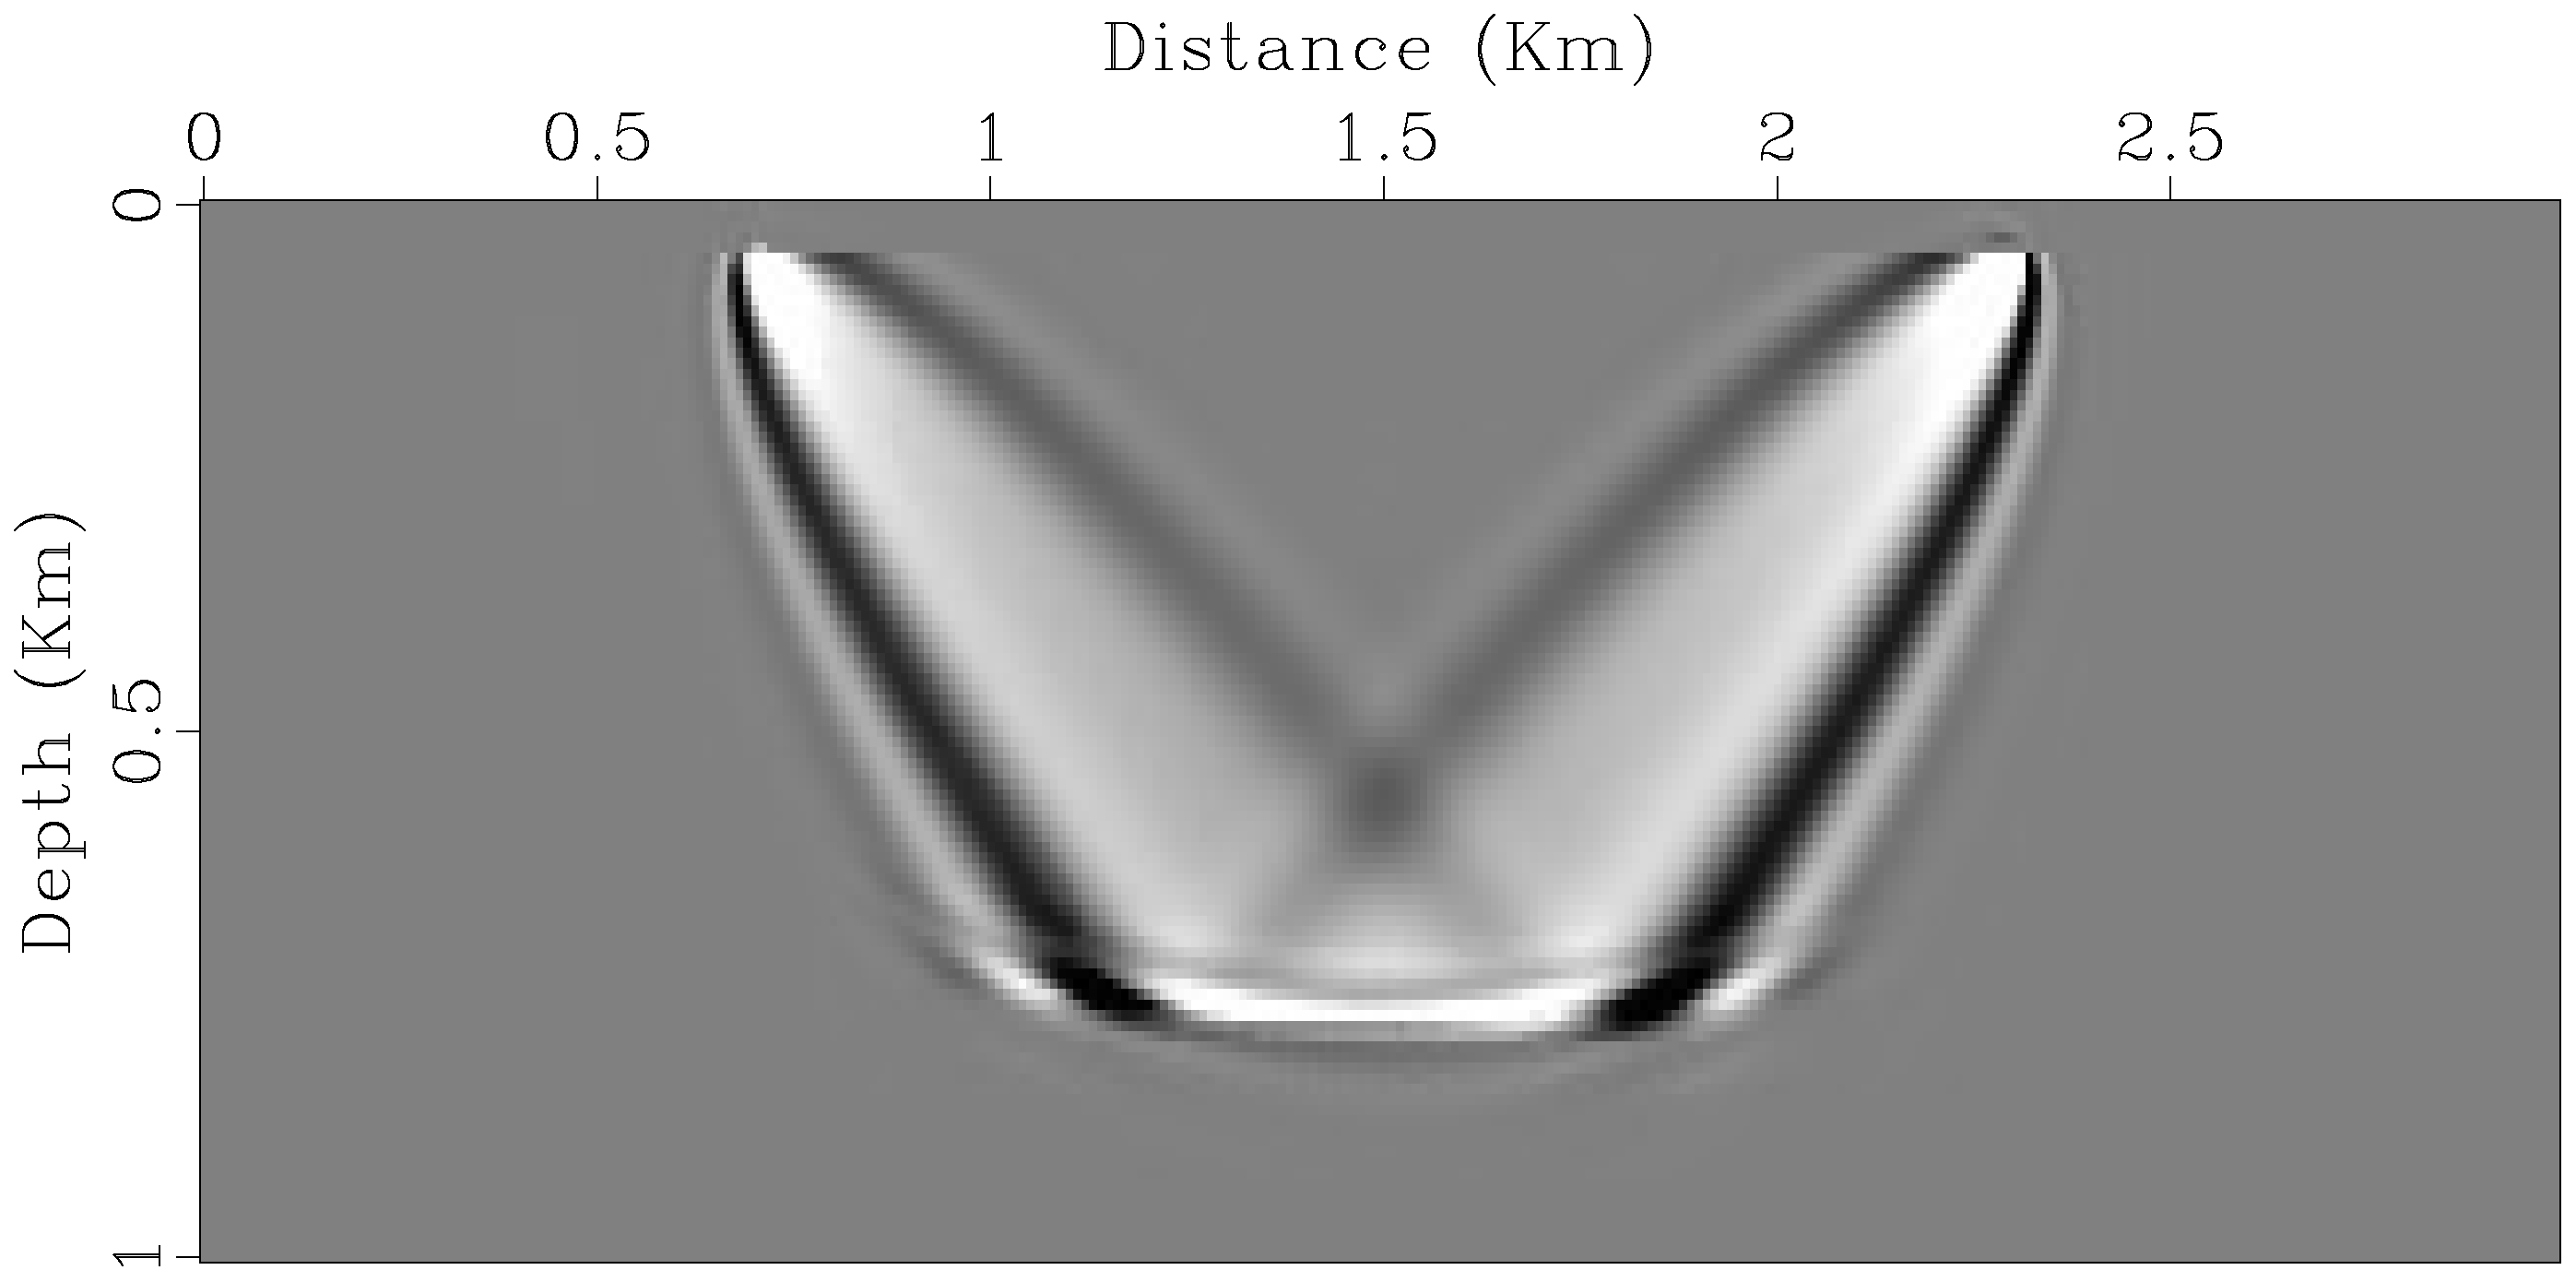
\includegraphics[width=0.49\linewidth]{figure/grad_rwi_poynting}}
    \subfigure[]{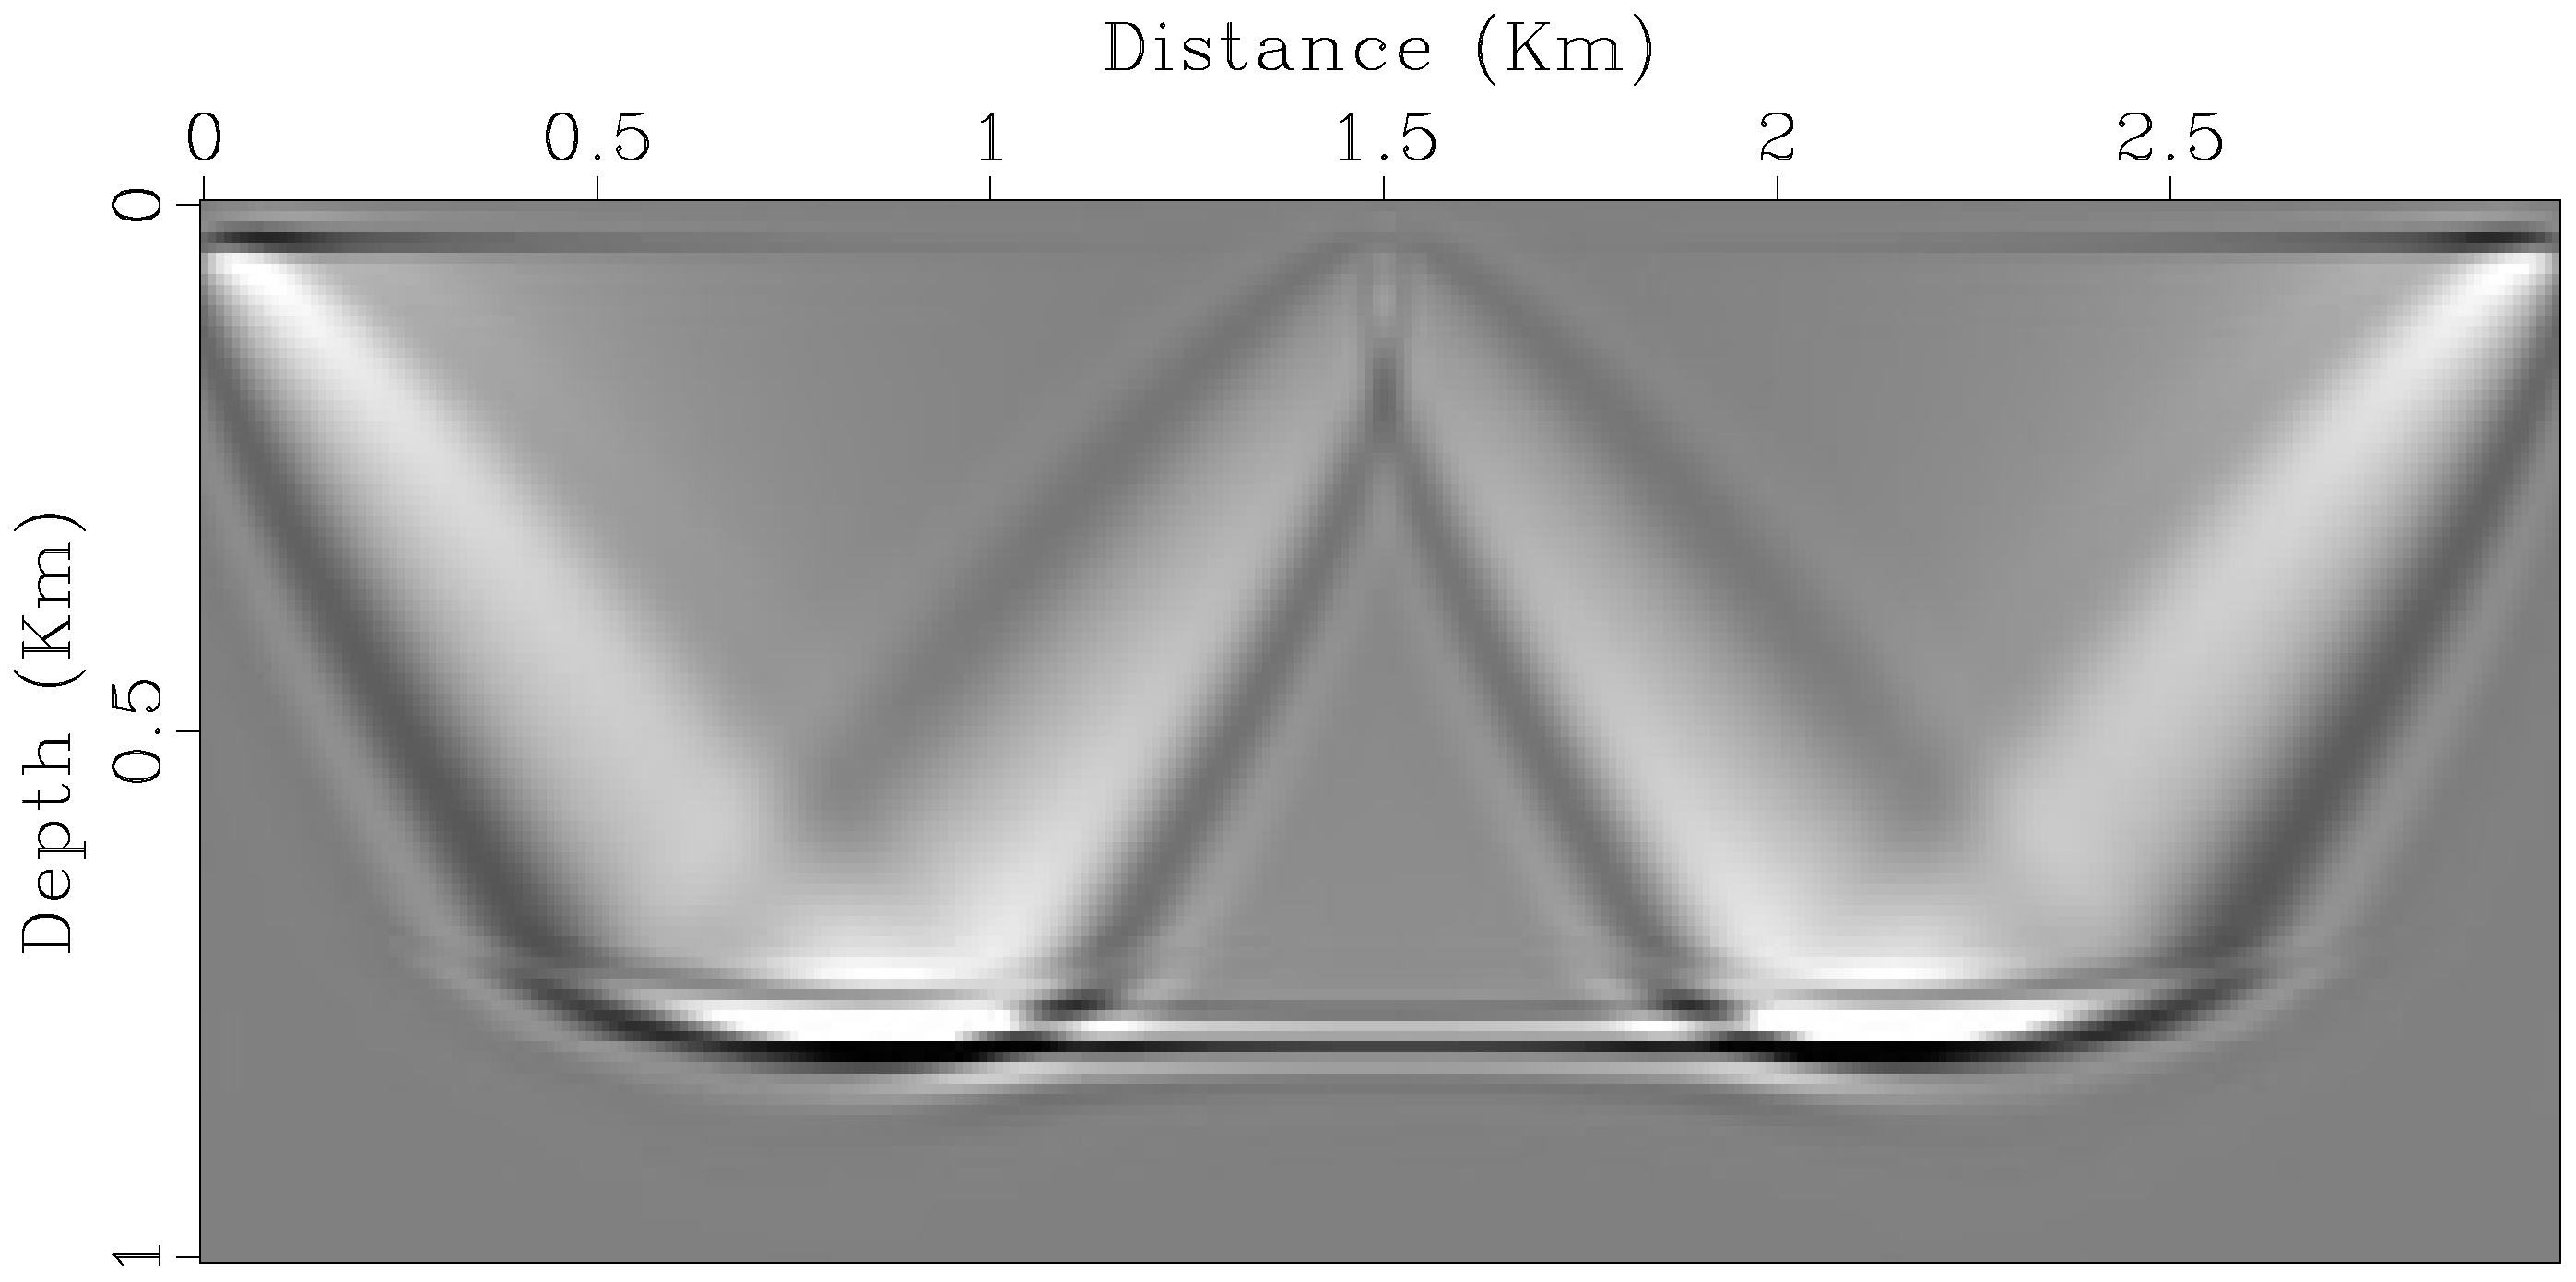
\includegraphics[width=0.49\linewidth]{figure/grad_rwi_oneshot}}
    \subfigure[]{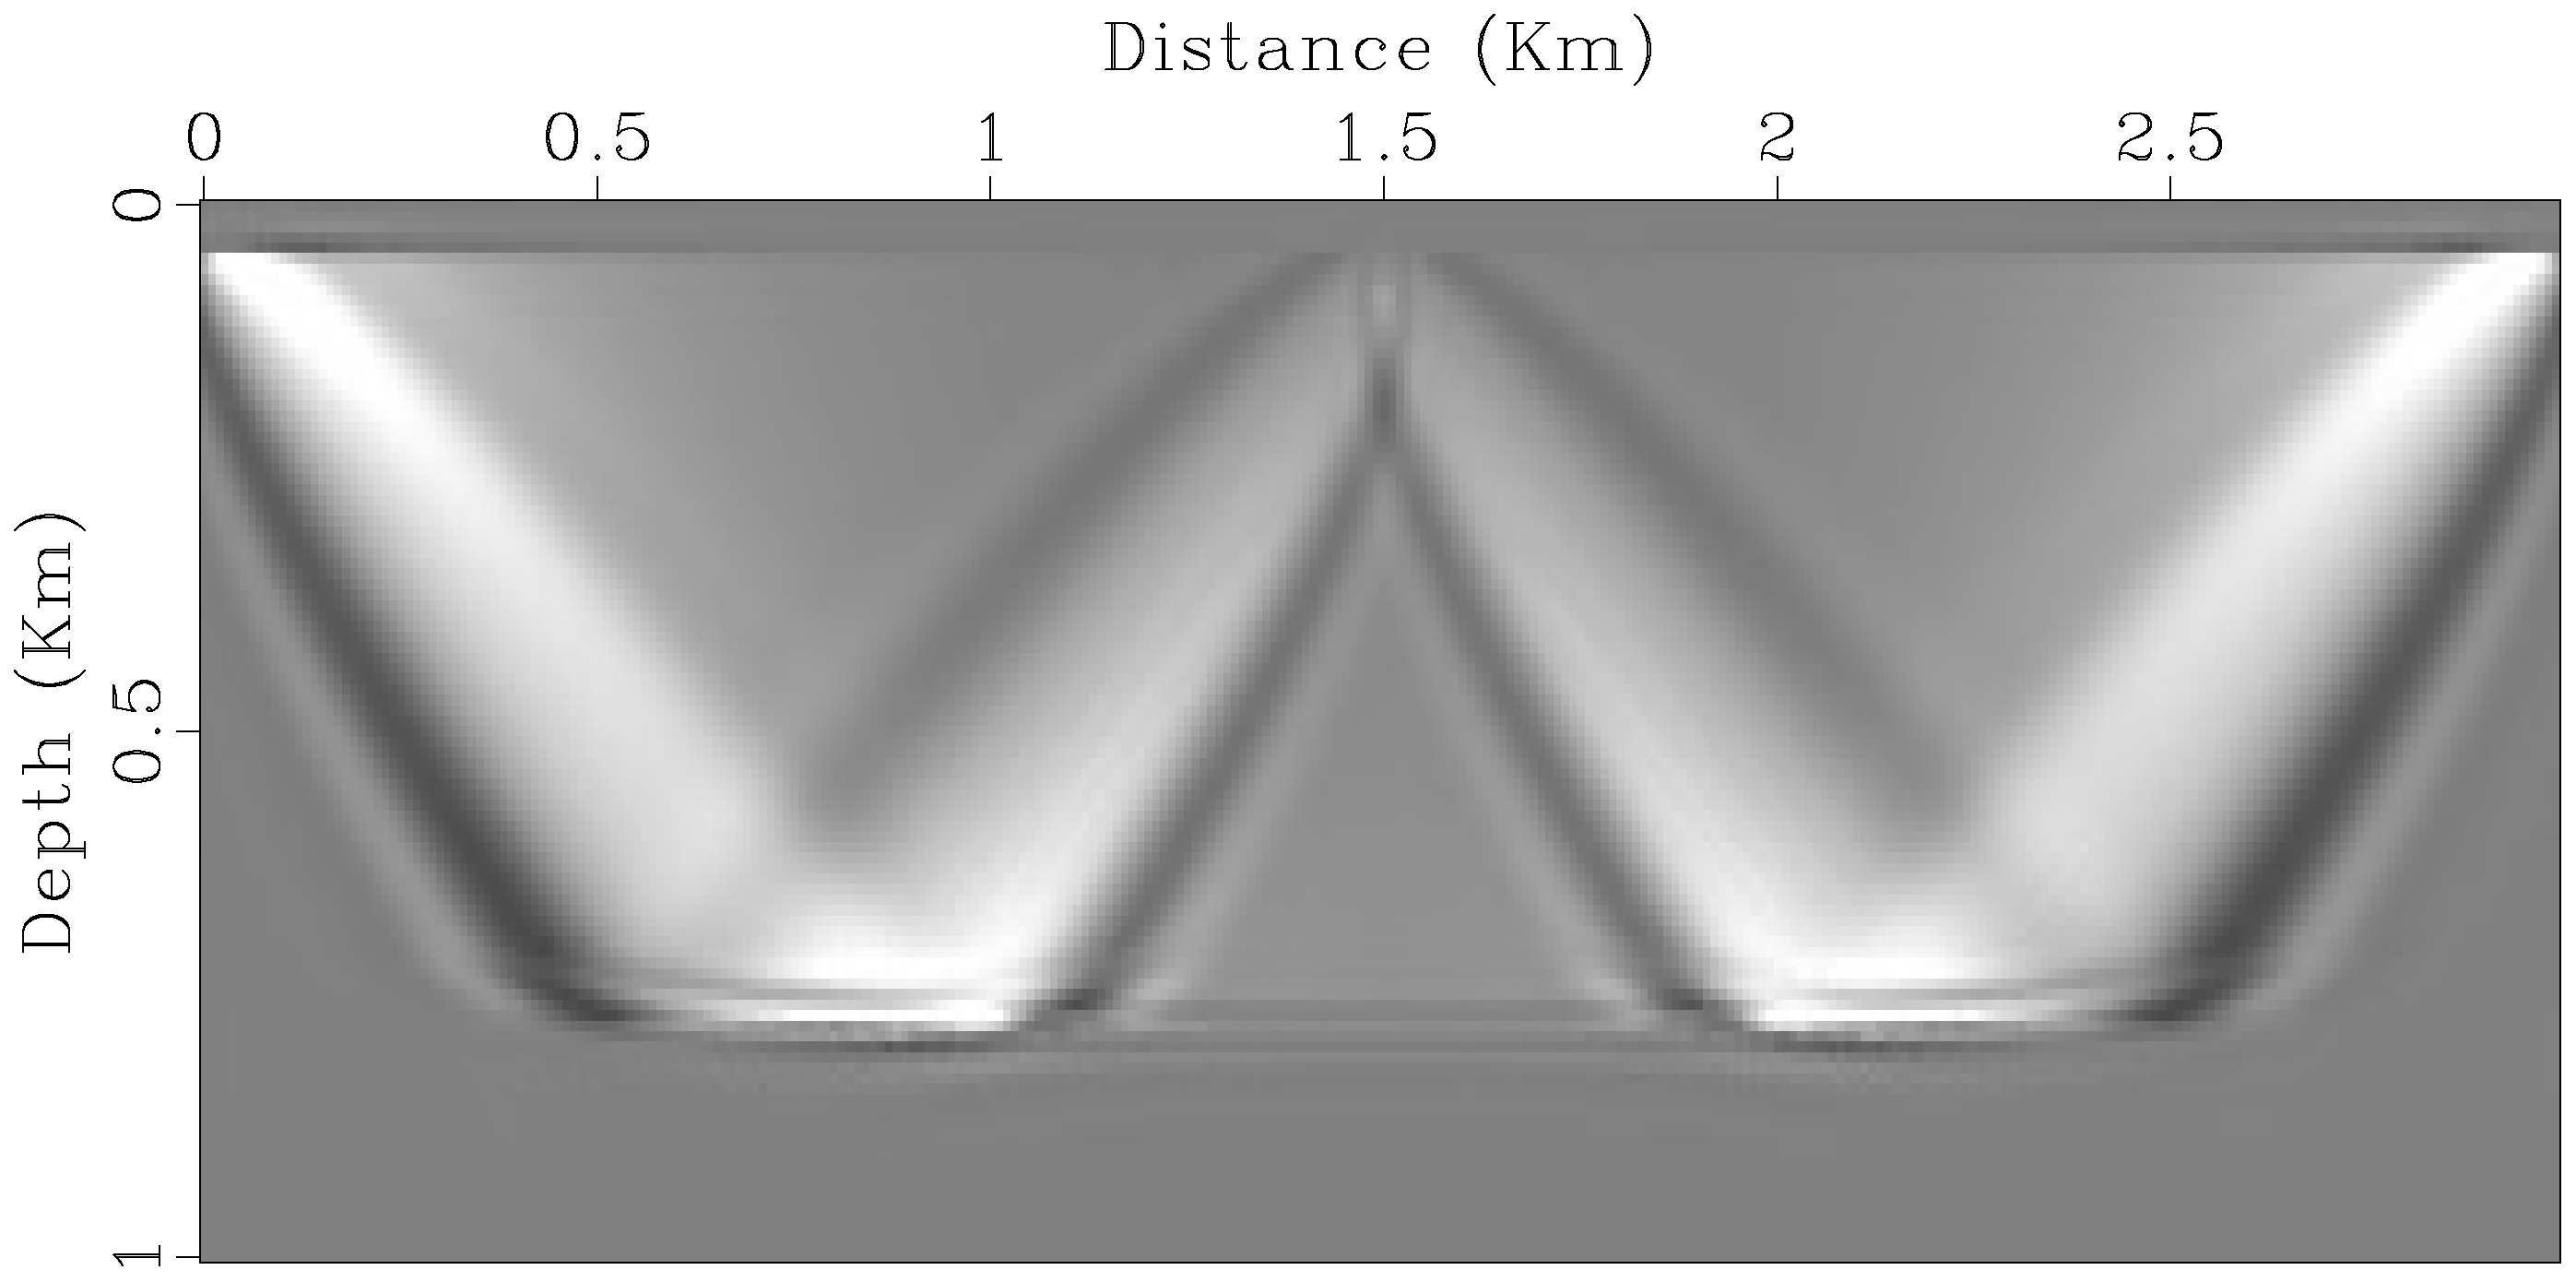
\includegraphics[width=0.49\linewidth]{figure/grad_rwi_poynting_oneshot}}
    \subfigure[]{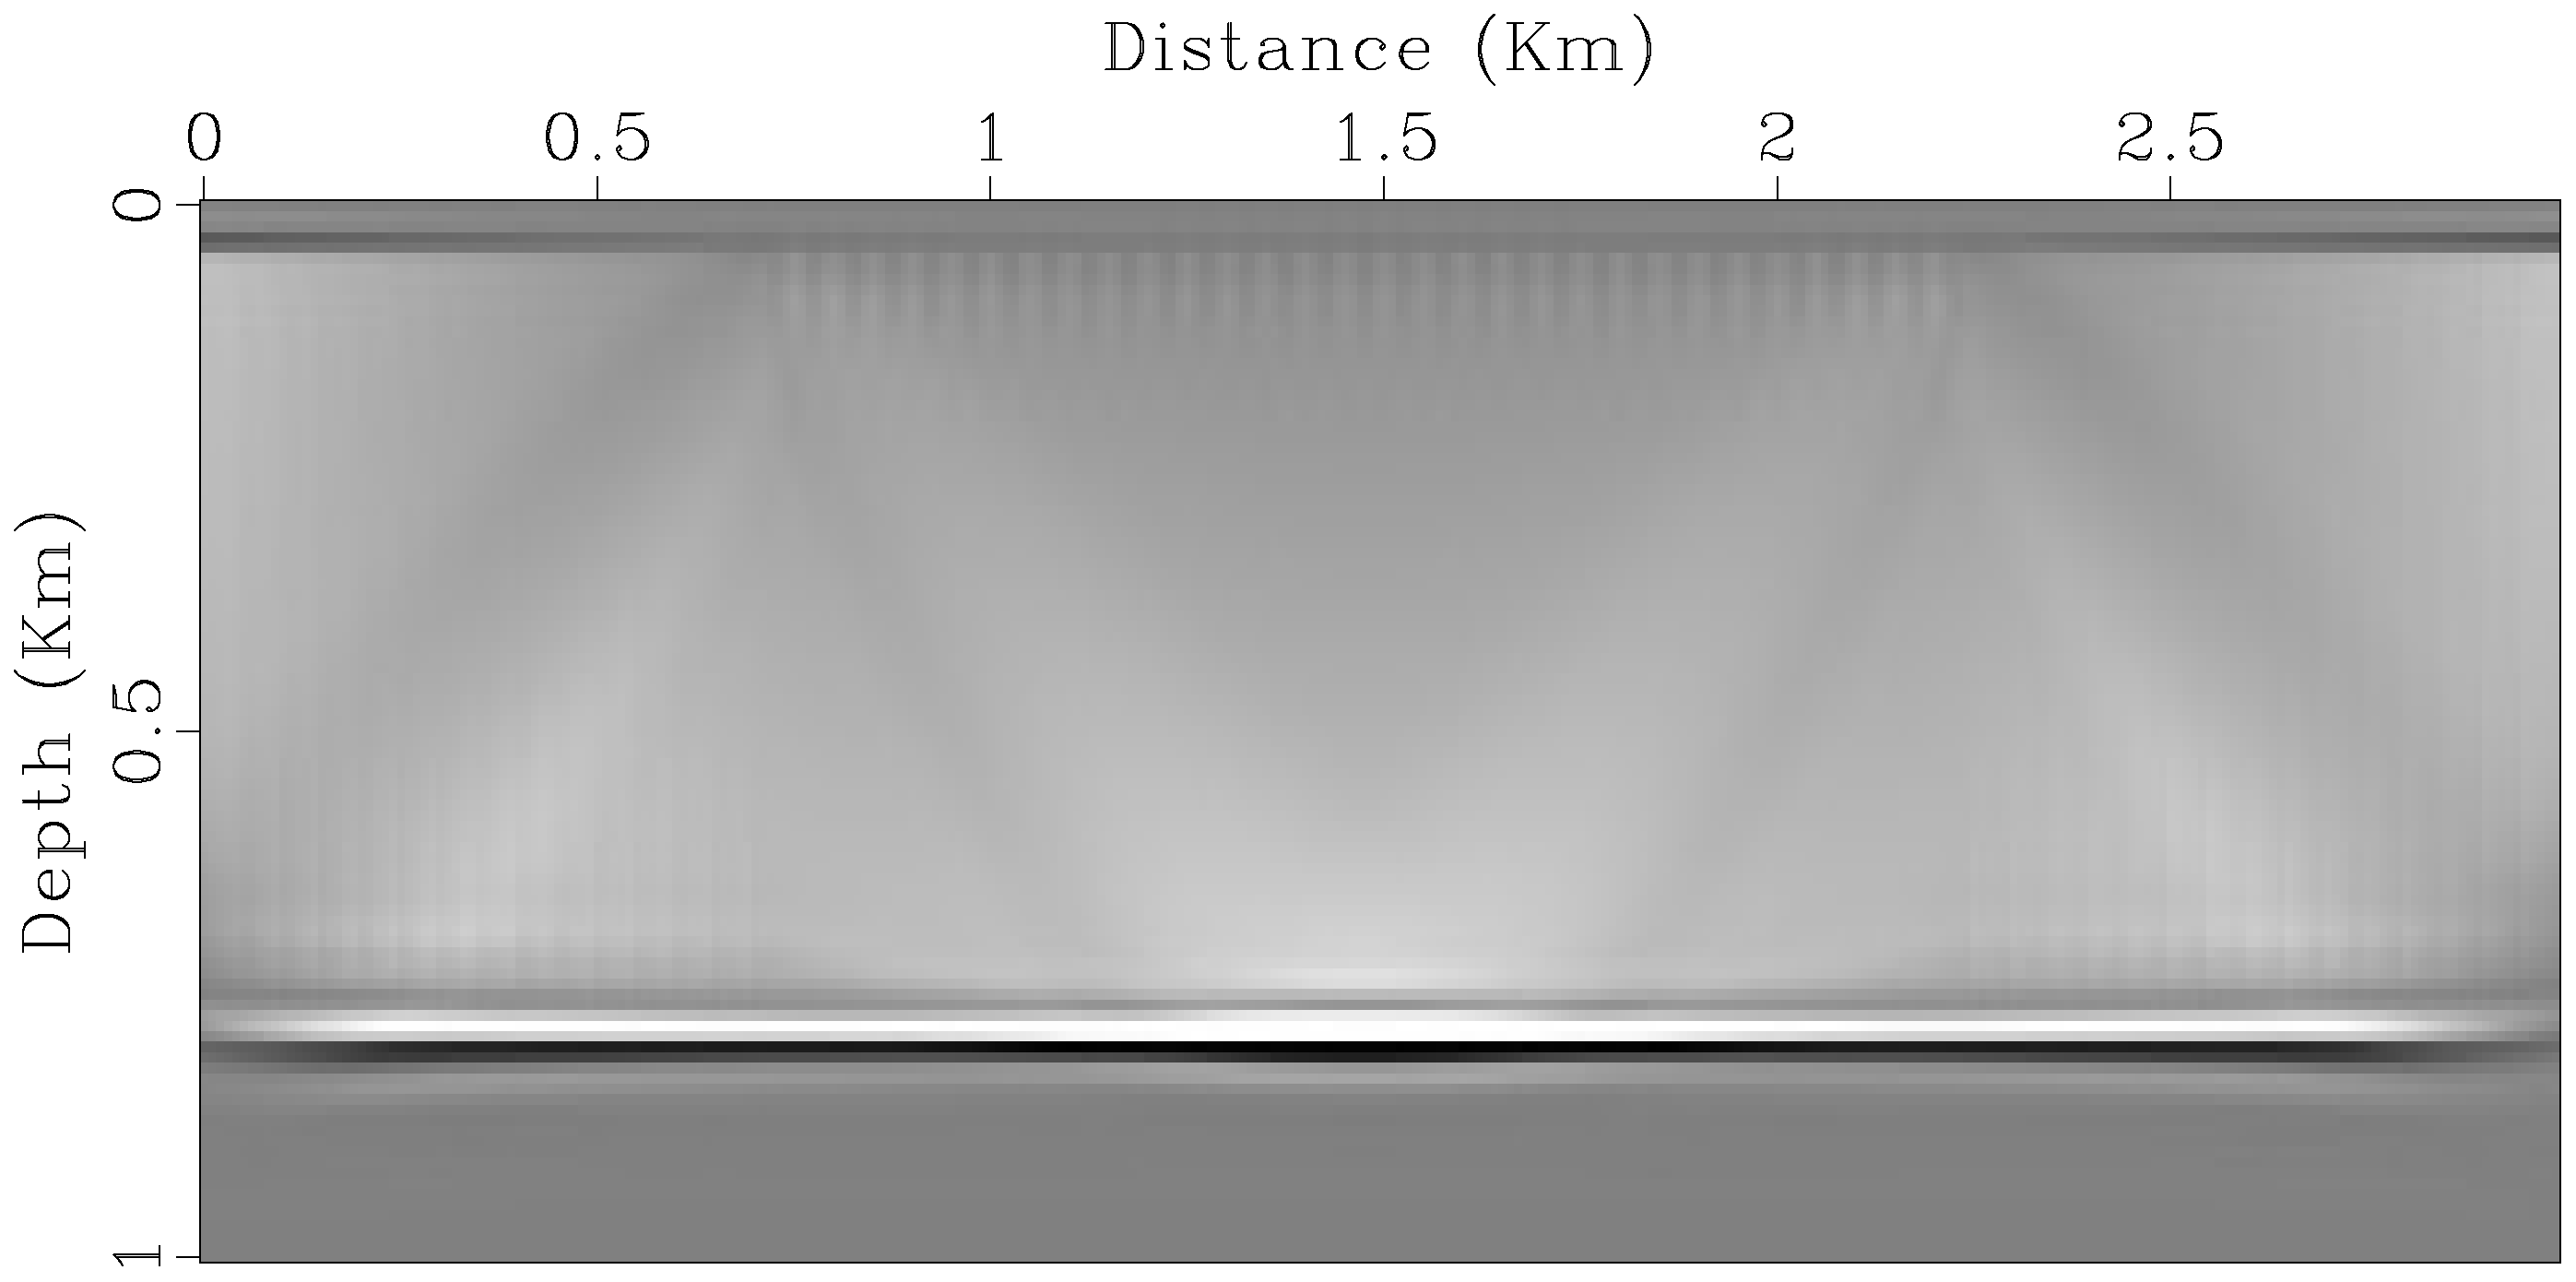
\includegraphics[width=0.49\linewidth]{figure/grad}}
    \subfigure[]{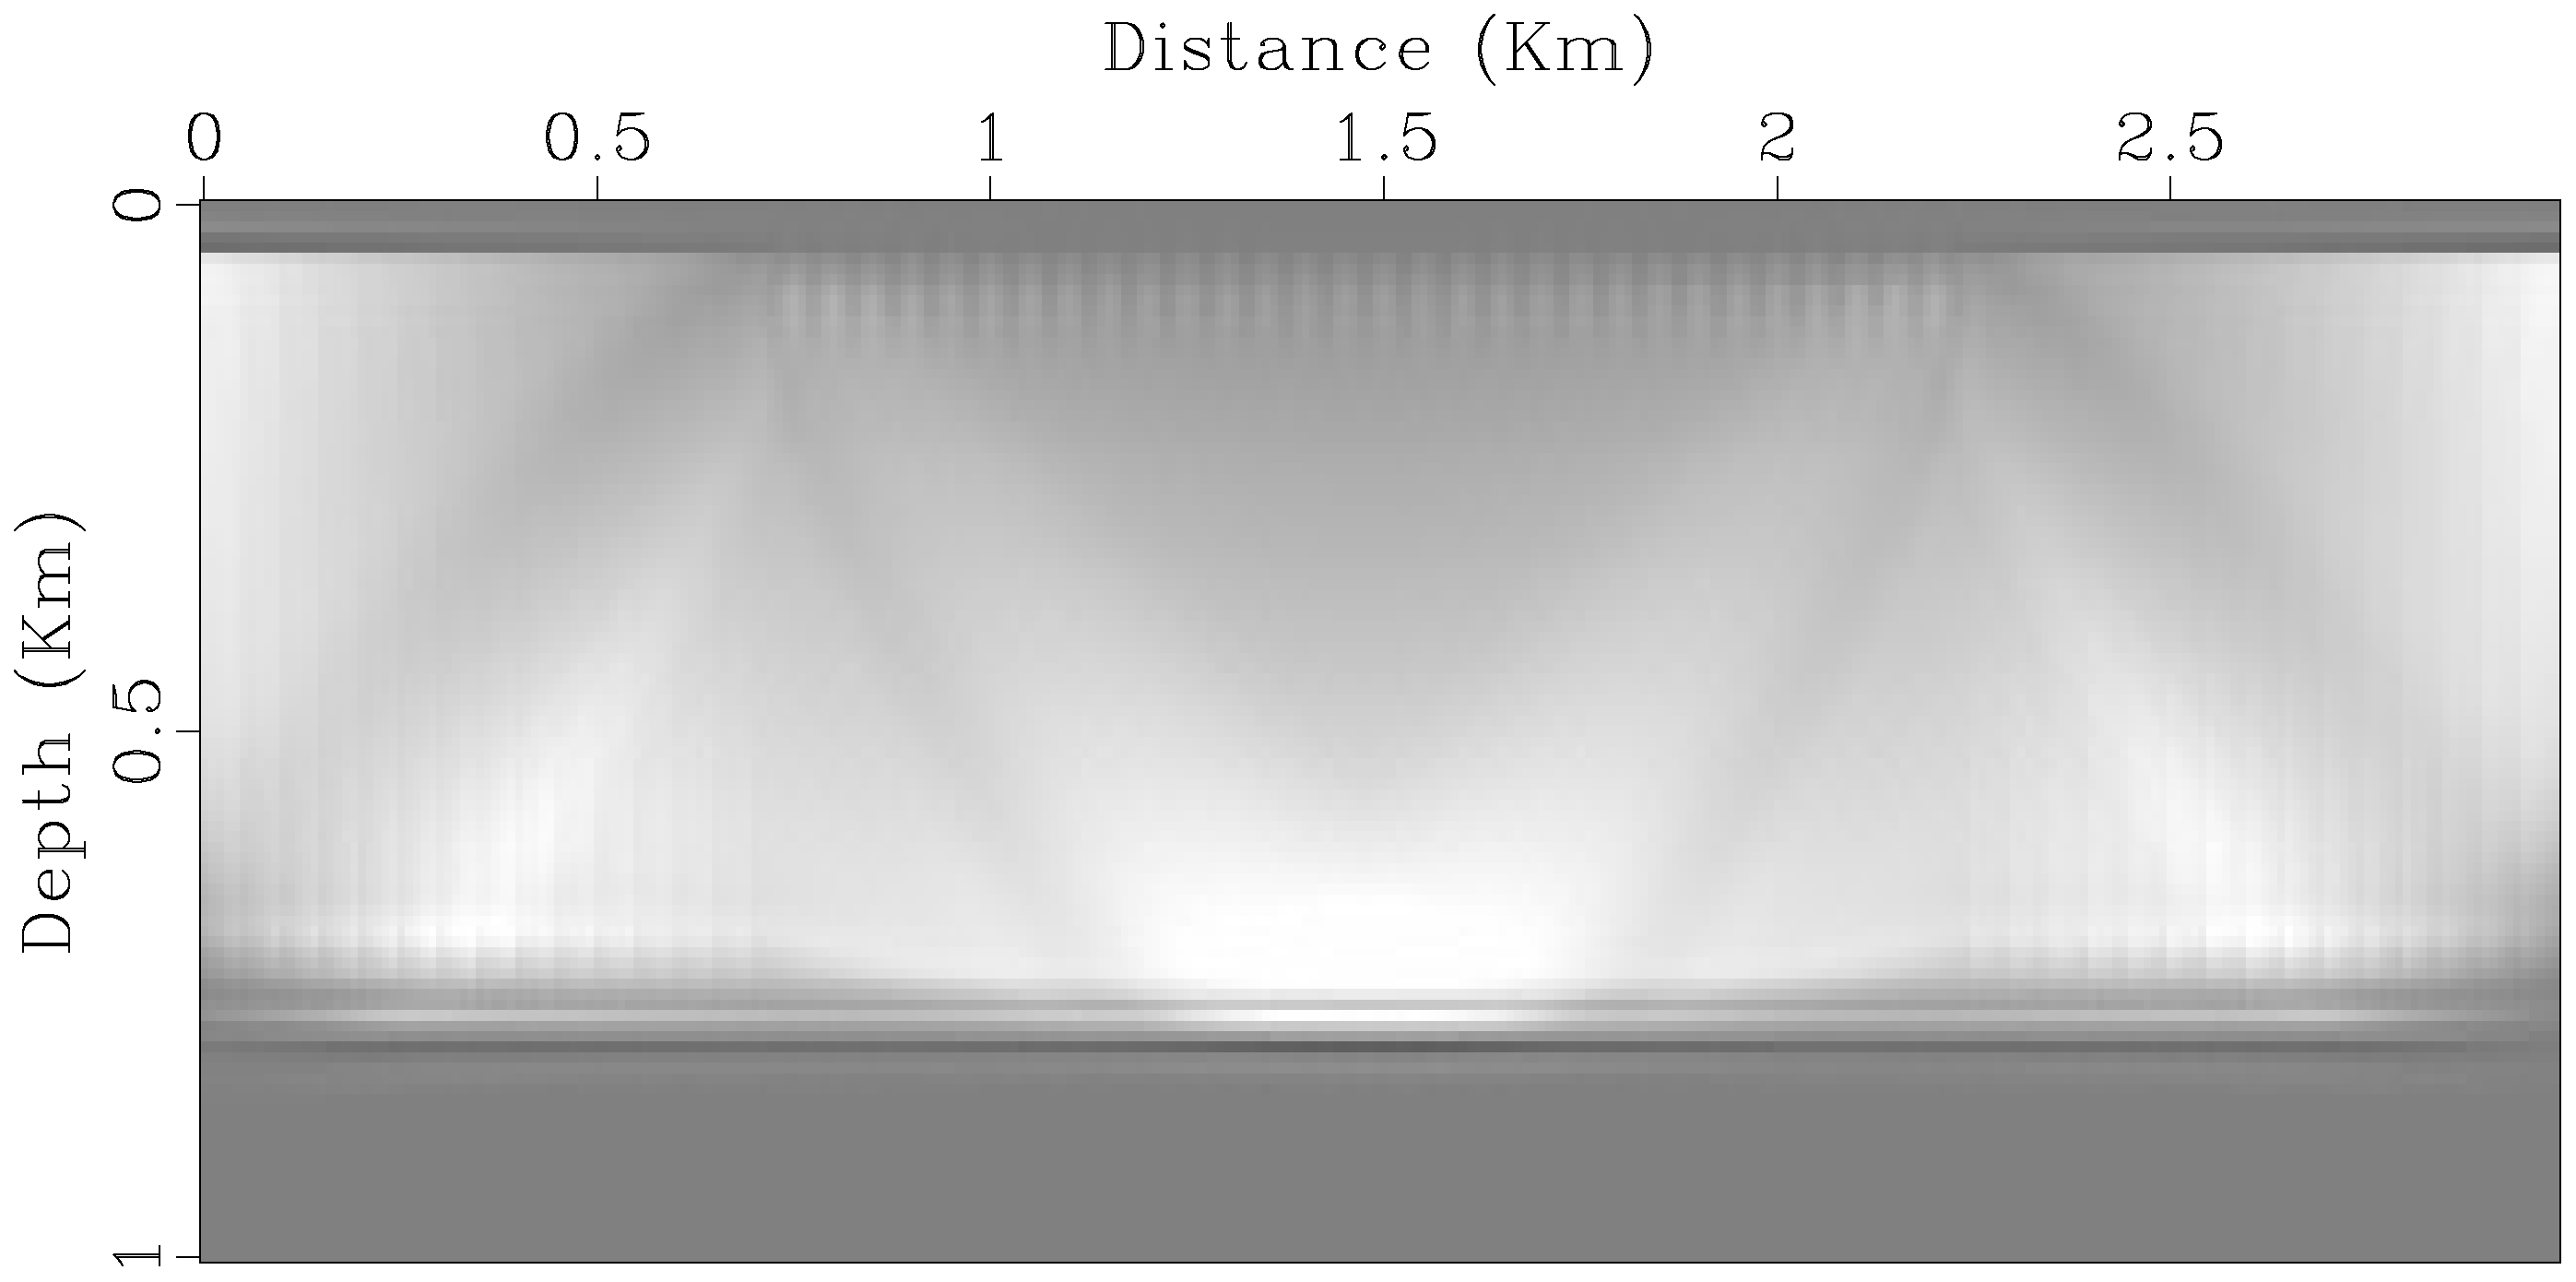
\includegraphics[width=0.49\linewidth]{figure/grad_poynting}}
    \fcaption{两层介质Poynting矢量预条件梯度对比,左边是没有预条件的梯度,右边是通过
	Poynting矢量上下行波分离预条件的梯度。(a,b)单炮单道;(c,d)单炮多道;
	(e,f)多炮多道。}{Comparison the gradients before and after using Poynting vector 
	for preconditing for simple two-layer model, the left column are before precondition 
	gradients and the righ column are after precondition results. (a, b) one shot and one 
	trance; (c, d) one shot and multi-trances; (e, f) multi-shots and multi-trances. 
	}[两层介质Poynting矢量预条件梯度对比]
    \label{fig:grad_poynting}
\end{figure*}

计算出梯度之后,$\tau(\mathbf{x})$可用最速下降法来迭代求解:
\begin{equation}
    \tau(\mathbf{x})^{(k+1)}=\tau(\mathbf{x})^k-\alpha \mathbf{P_c}(\mathbf{x})
    \frac{\partial \mathcal{L}}{\partial \tau(\mathbf{x})},
\end{equation}
式中$k$是迭代次数,$\mathbf{P}_c(\mathbf{x})$是预条件算子,步长$\alpha$可通过
任何反向追踪的线性搜索方法求解(\citeA{nocedal:1999})。在每一个迭代步内,
当$\tau(\mathbf{x})$更新之后可用方程~\ref{eq:tq}将其转换为$Q(\mathbf{x})$。


\newpage
\section{数值实验}
本节用一个层状模型(图~\ref{fig:lens_model})来验证$Q$-RWI的有效性。该模型
宽4km,深2.5km。在模型的表面均匀分布20炮,炮间距为200m,检波器对称分布于震源
的两端,间距为10m且最大偏移距为1km。用峰值频率为30Hz的雷克子波作为爆炸震源。
在模型的中深部包含一个强的$Q$异常体,最小$Q$值达到30。在反演的过程中认为体积
模量$K_0$和$\delta K$都是已知的,并且密度为常数。用均匀模型($Q=200$)作为
初始模型。

如图~\ref{fig:lens_model}c~所示,经过30次迭代之后,$Q$-RWI基本恢复了中深部
的$Q$异常。图~\ref{fig:chouxian}分别抽取了$x=1$km、2km、3km处的伪井曲线。
抽线的结果进一步证明了$Q$-RWI对中深部异常$Q$的恢复能力。由于反射数据在浅层
覆盖不够即波路径在近地表处变窄,使得$Q$-RWI在浅层只能得到一个光滑的等效解。
这也证实了地球物理反问题解的多解性,要处理好这种多解性,在反演时必需加入
先验信息的约束或者多种反演方法相结合,例如$Q$-FWI就能很好的反演浅层$Q$模型。
在模型的最底部,由于没有接收到反射数据,反射波路径没有穿过该区域,所以没法
正确反演。图~\ref{fig:misfit_model}展示了迭代过程中的收敛曲线,在这种理想
的合成数据中,目标泛函下降了七八个数量级,这也有力的证实了$Q$-FWI框架的合理
性。图~\ref{fig:record_diff}展示了在$x=2$km 处第10炮观测记录;观测数据与初始
模型模拟数据的残差以及观测记录与30次迭代之后模拟数据的残差。经过30次迭代之后
模拟数据与观测数据之间的残差基本为零,这也更好的证明了$Q$-RWI的有效性。

最后,我们用$Q$补偿的RTM来验证反演结果的可靠性。图~\ref{fig:rtm_model}
分别展示了初始$Q$模型补偿的RTM成像结果、真实$Q$模型补偿的RTM成像结果
以及反演$Q$模型补偿的RTM成像结果。从成像结果中可以看出,初始$Q$模型补偿的RTM
(图~\ref{fig:rtm_model}a)在强衰减区域能量损失严重,并且由于速度频散的影响其成像位
置不对。准确的$Q$模型不仅补偿了强衰减区损失的能量(图~\ref{fig:rtm_model}b),而且也
保持衰减介质中的速度频散关系,从而保证了成像位置的正确性。用$Q$-RWI反演的$Q$模型
补偿的RTM结果(图~\ref{fig:rtm_model}c)与用真实$Q$模型补偿的RTM具有相当的成像
结果。这也从$Q$补偿成像的角度证明了$Q$-RWI反演结果的可靠性。


\begin{figure*}[!htbp]
    \centering
    %{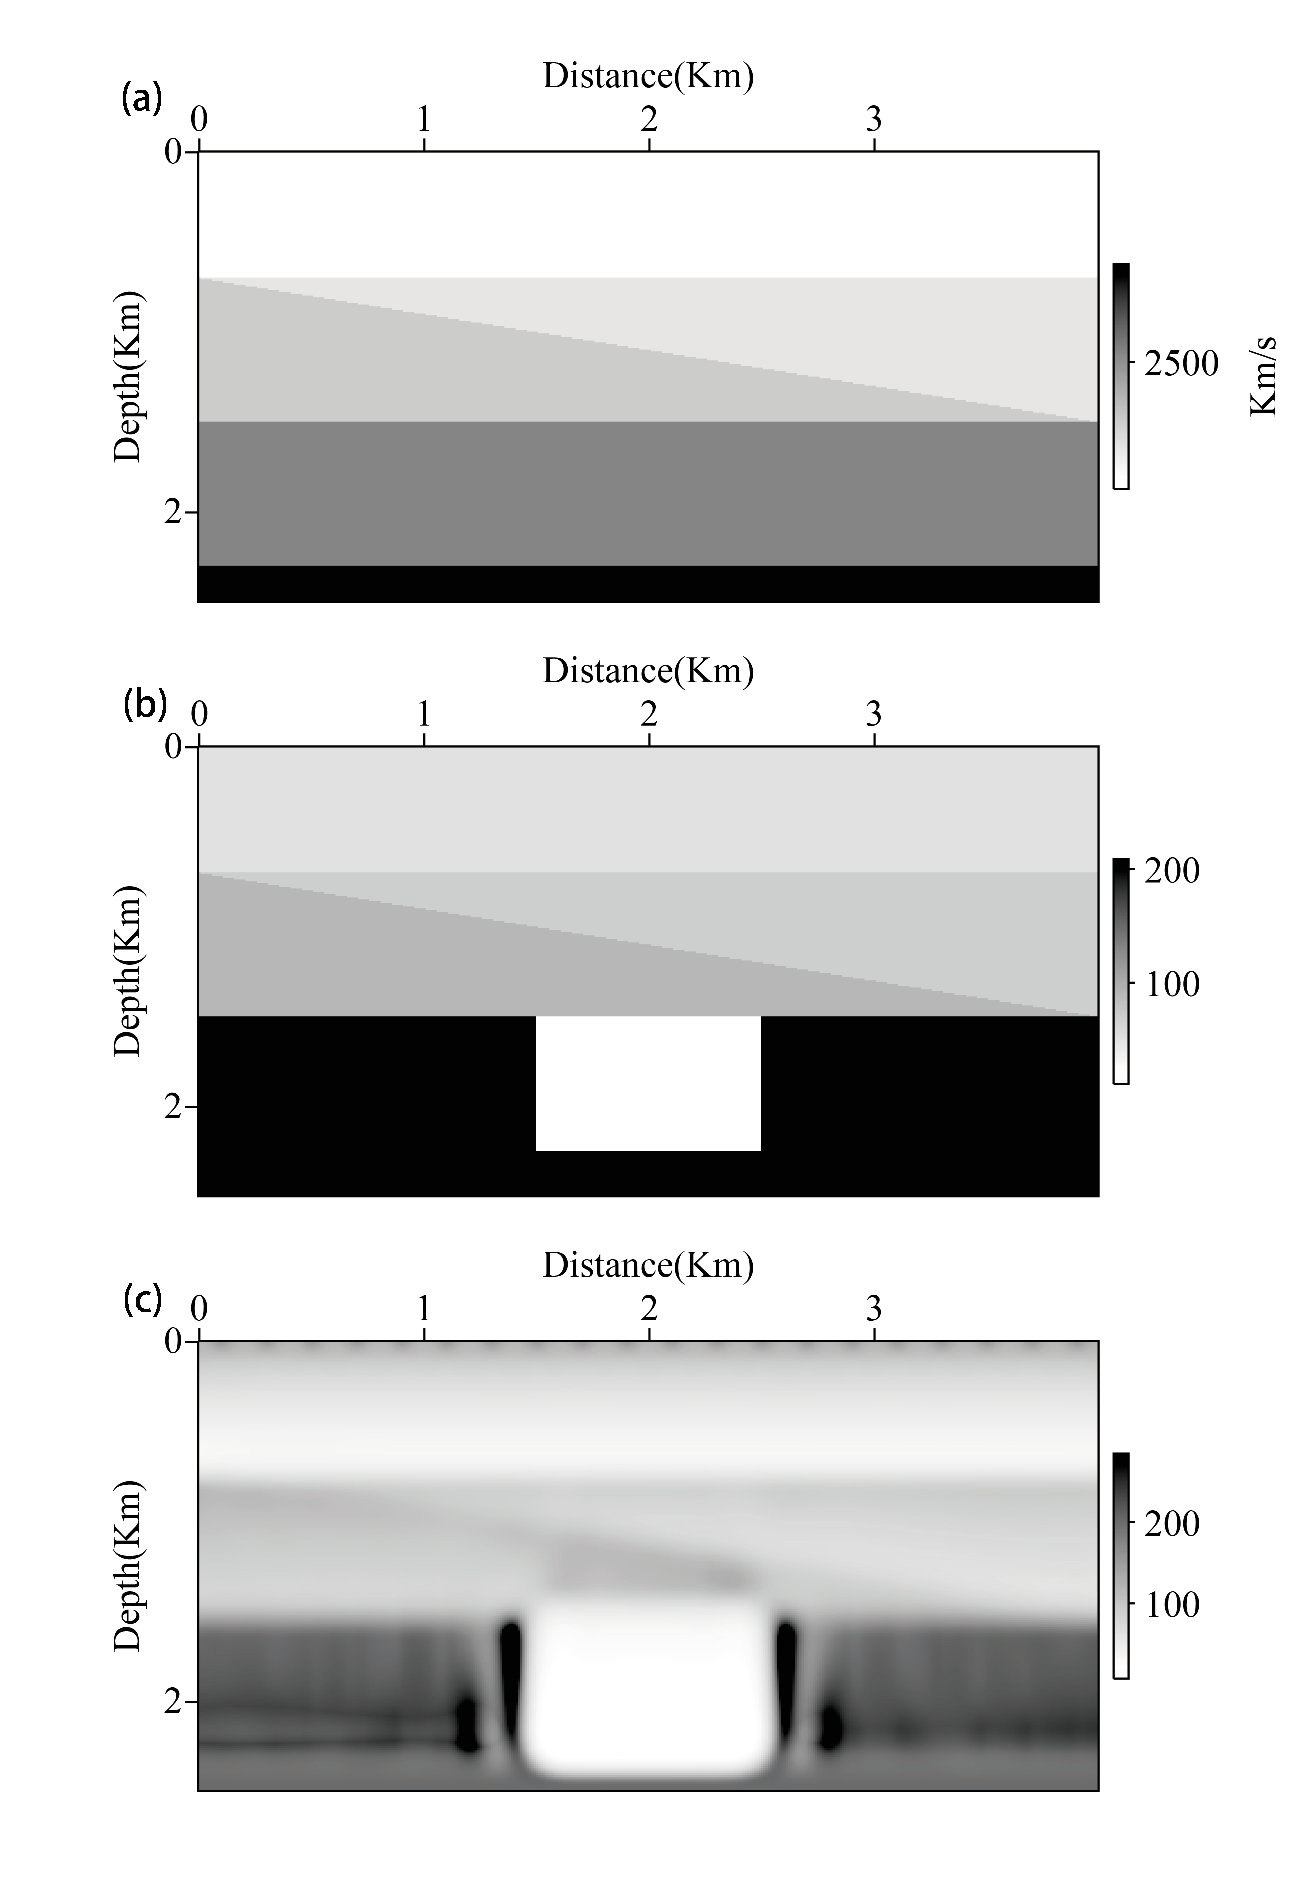
\includegraphics[width=0.85\linewidth]{figure/model}}
	\subfigure[]{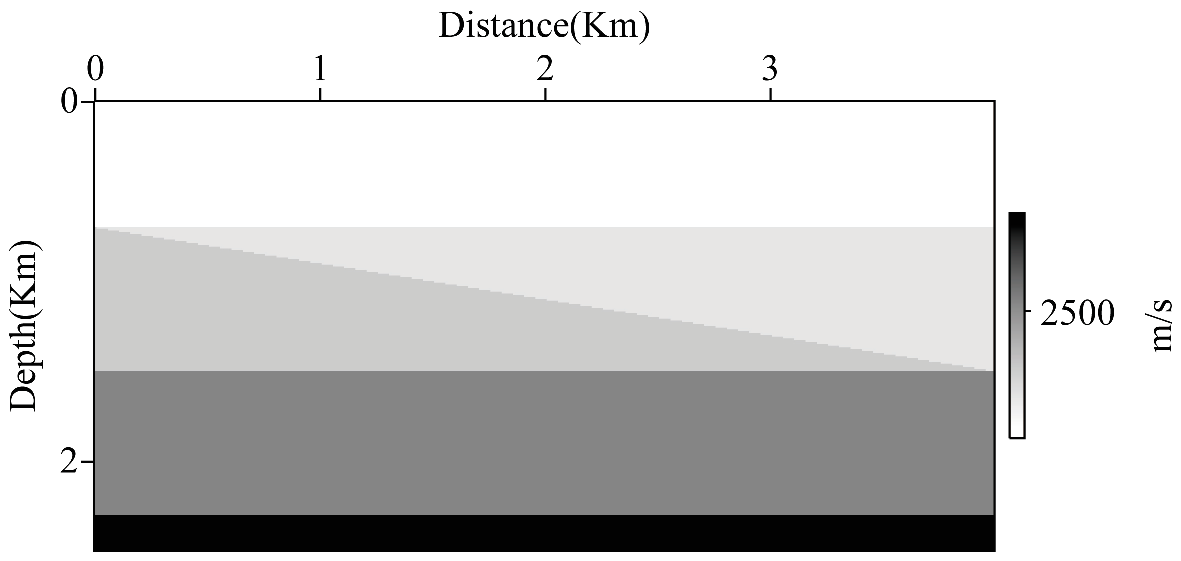
\includegraphics[width=0.82\linewidth]{figure/vel_400x250}}
	\subfigure[]{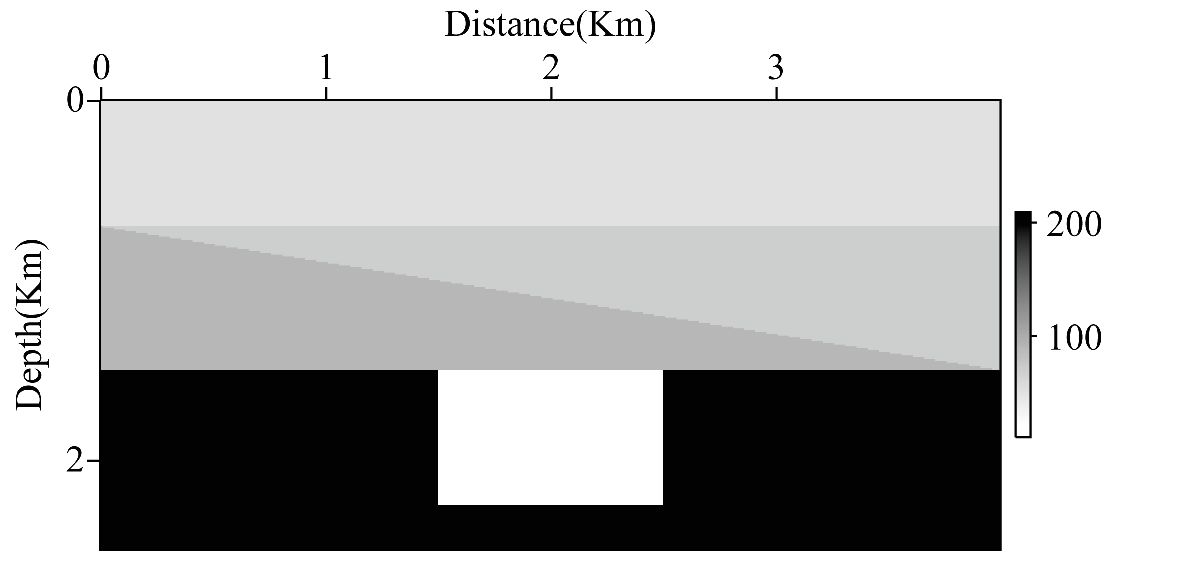
\includegraphics[width=0.82\linewidth]{figure/q_400x250}}
	\subfigure[]{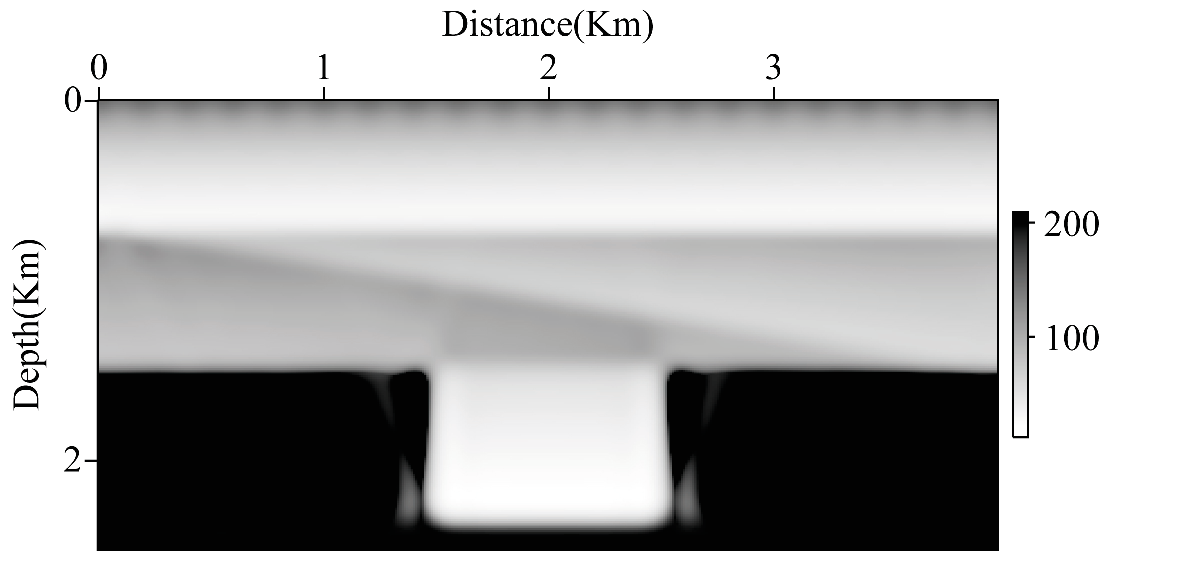
\includegraphics[width=0.82\linewidth]{figure/fq_400x250}}
	\fcaption{层状模型:(a)速度模型;(b)真实$Q$模型;(c)$Q$-RWI
	反演结果。}{The layered model:(a) the velocity model,
	(b) true $Q$ model and (c) inverted $Q$ model using $Q$-RWI.}
	[层状模型]
    \label{fig:lens_model}
\end{figure*}

\begin{figure*}[!htbp]
    \centering
	\subfigure[]{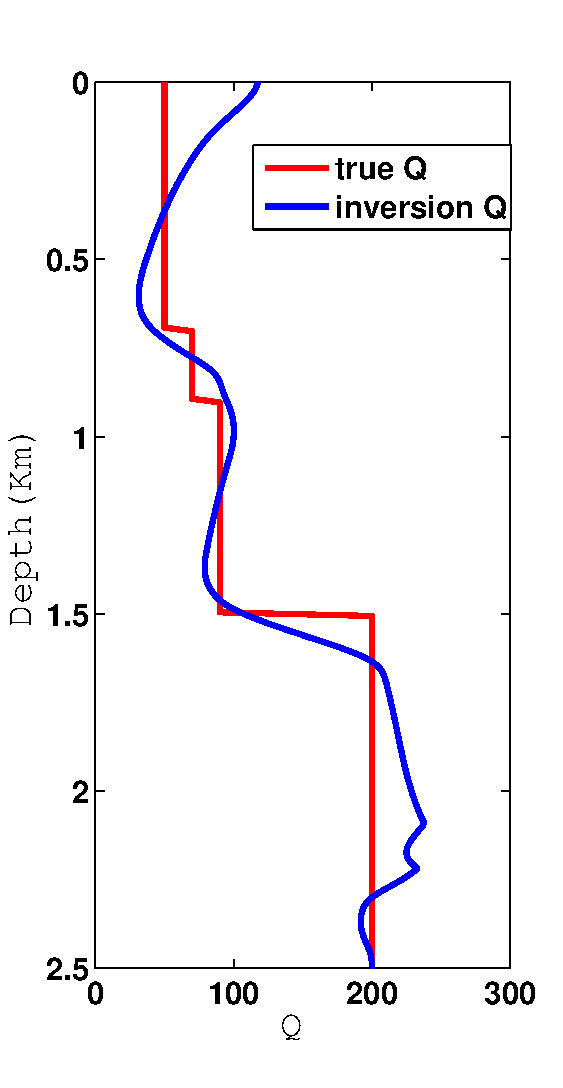
\includegraphics[width=0.32\linewidth]{figure/1km}}
	\subfigure[]{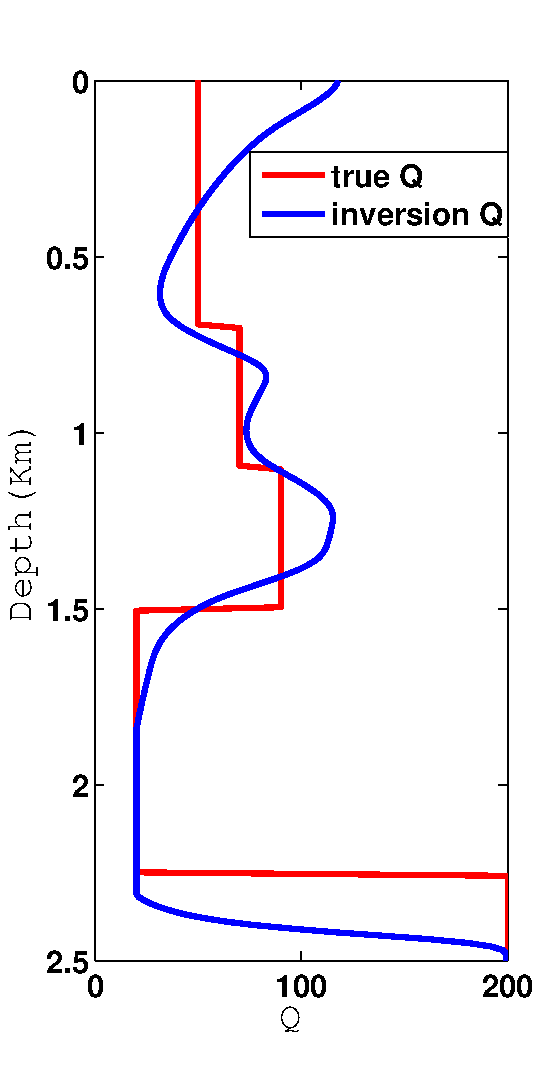
\includegraphics[width=0.32\linewidth]{figure/2km}}
	\subfigure[]{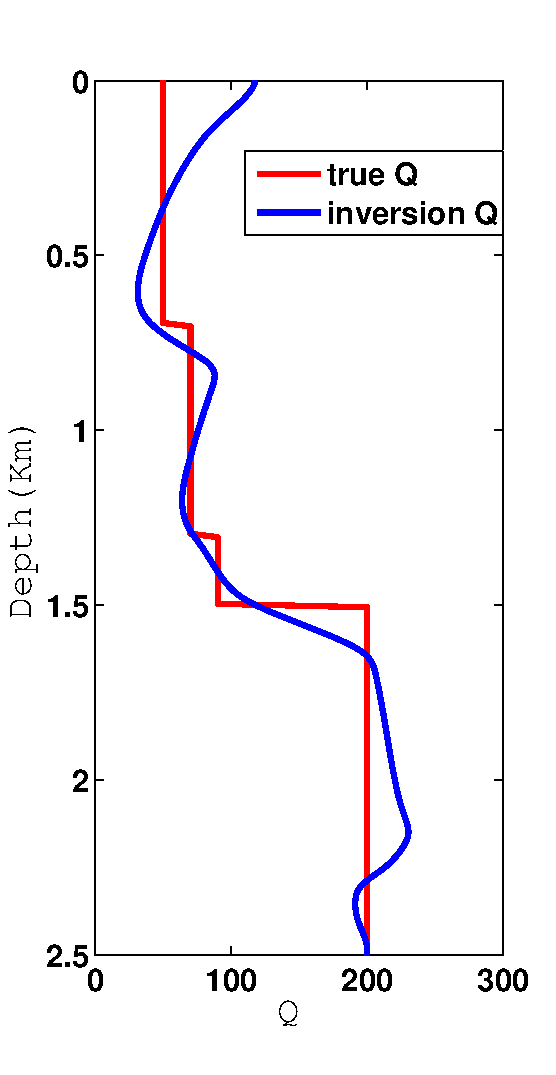
\includegraphics[width=0.32\linewidth]{figure/3km}}
	\fcaption{抽线对比:(a)1km处;(b)2km处;(c)3km处。}{Pseudowells comparison at (a) 1km, (b) 2km
	and (c) 3km.}[抽线对比结果]
    \label{fig:chouxian}
\end{figure*}

\begin{figure*}[!htbp]
    \centering
    {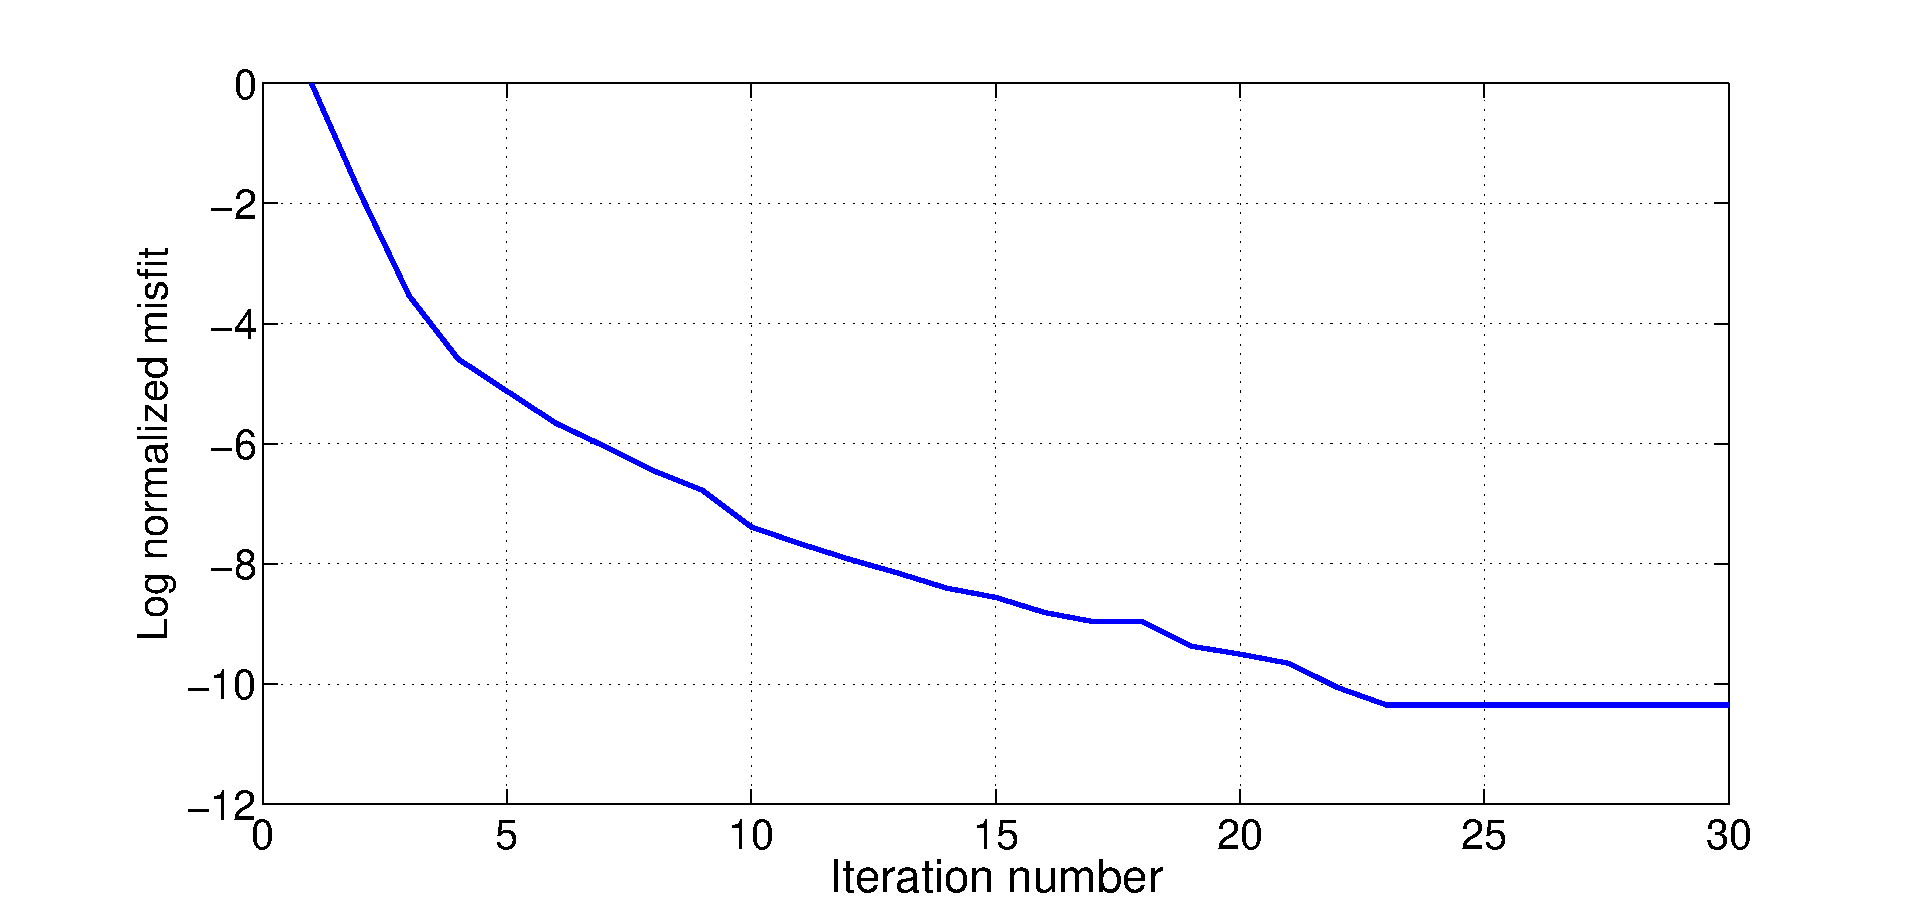
\includegraphics[width=1.0\linewidth]{figure/misfit}}
    \fcaption{收敛曲线}{The history of convergence.}[收敛曲线]
    \label{fig:misfit_model}
\end{figure*}

\begin{figure*}[!htbp]
    \centering
	\subfigure[]{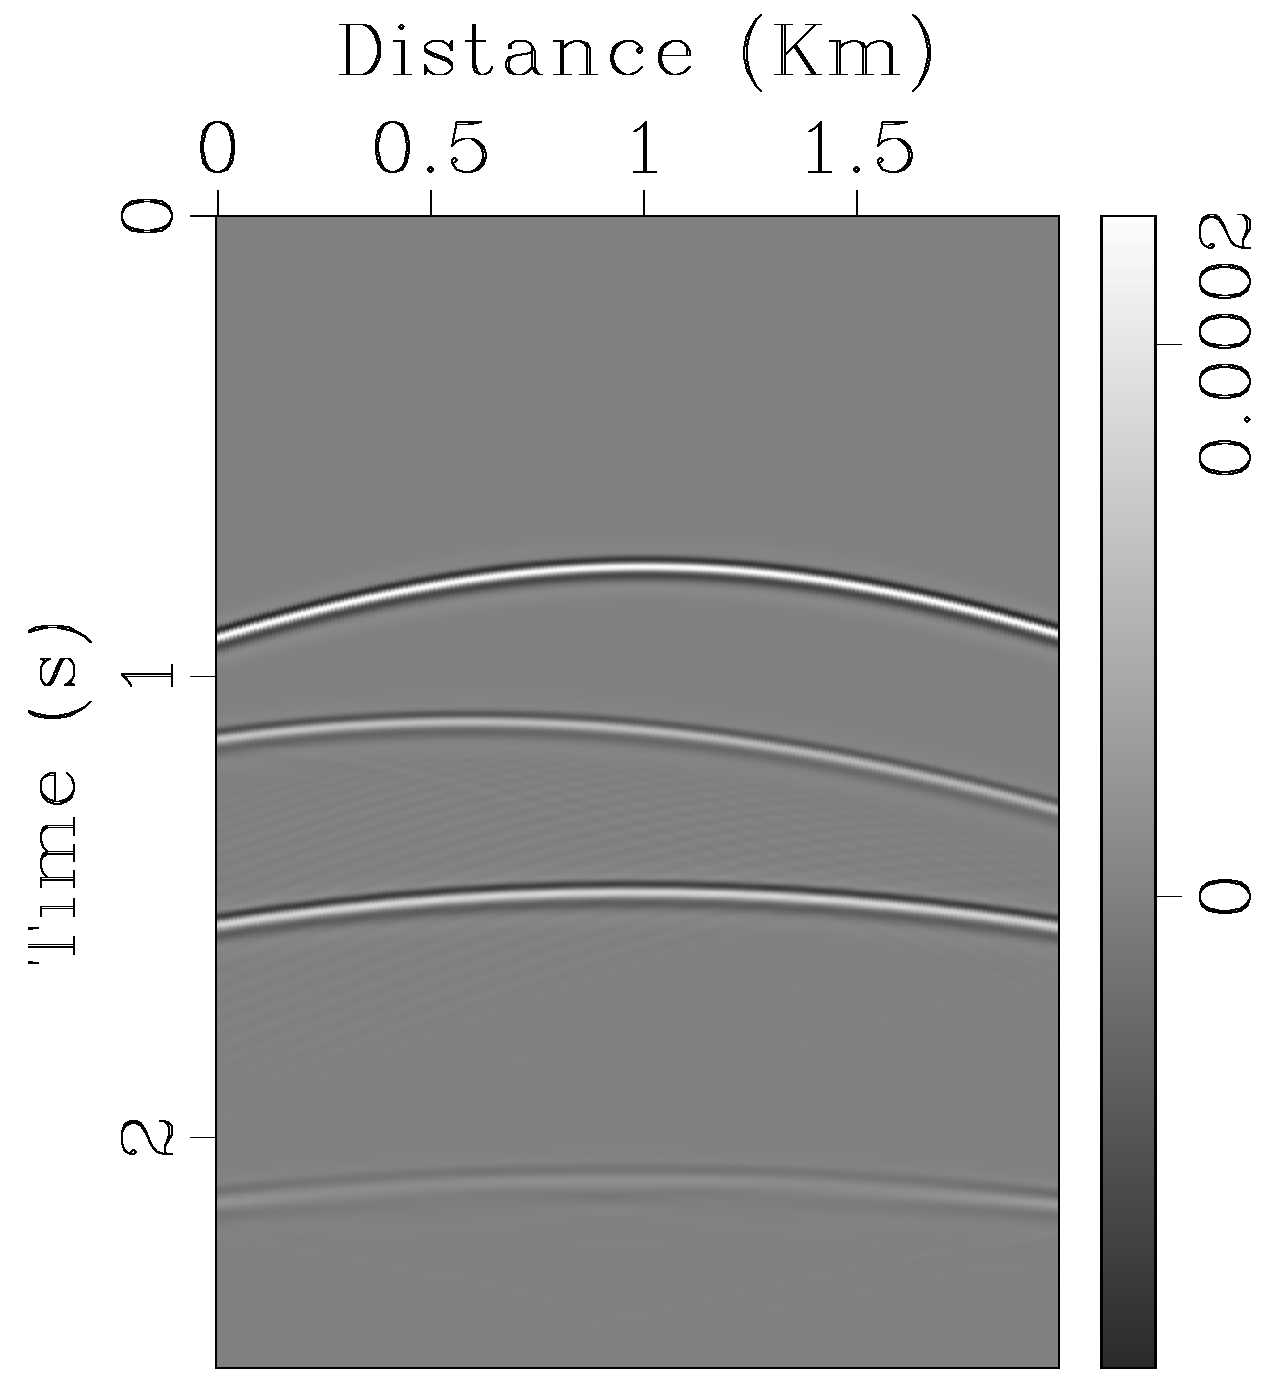
\includegraphics[width=0.47\linewidth]{figure/record}}
	\subfigure[]{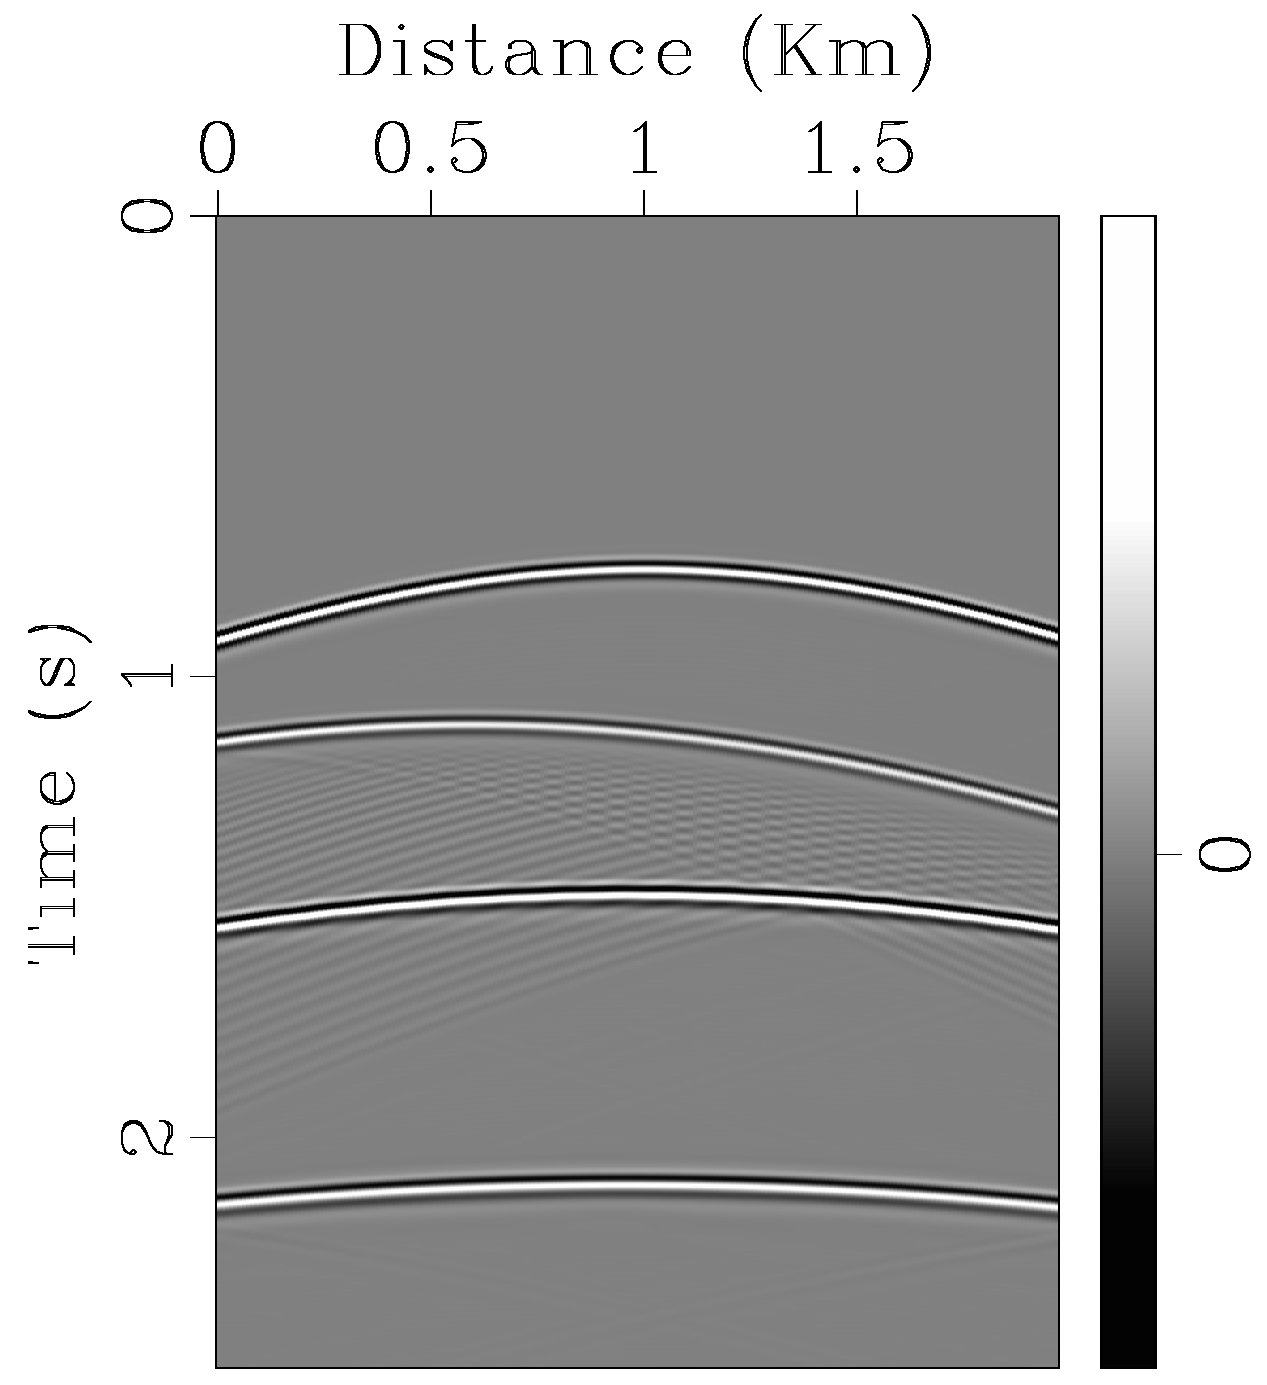
\includegraphics[width=0.47\linewidth]{figure/diff0}}
	\subfigure[]{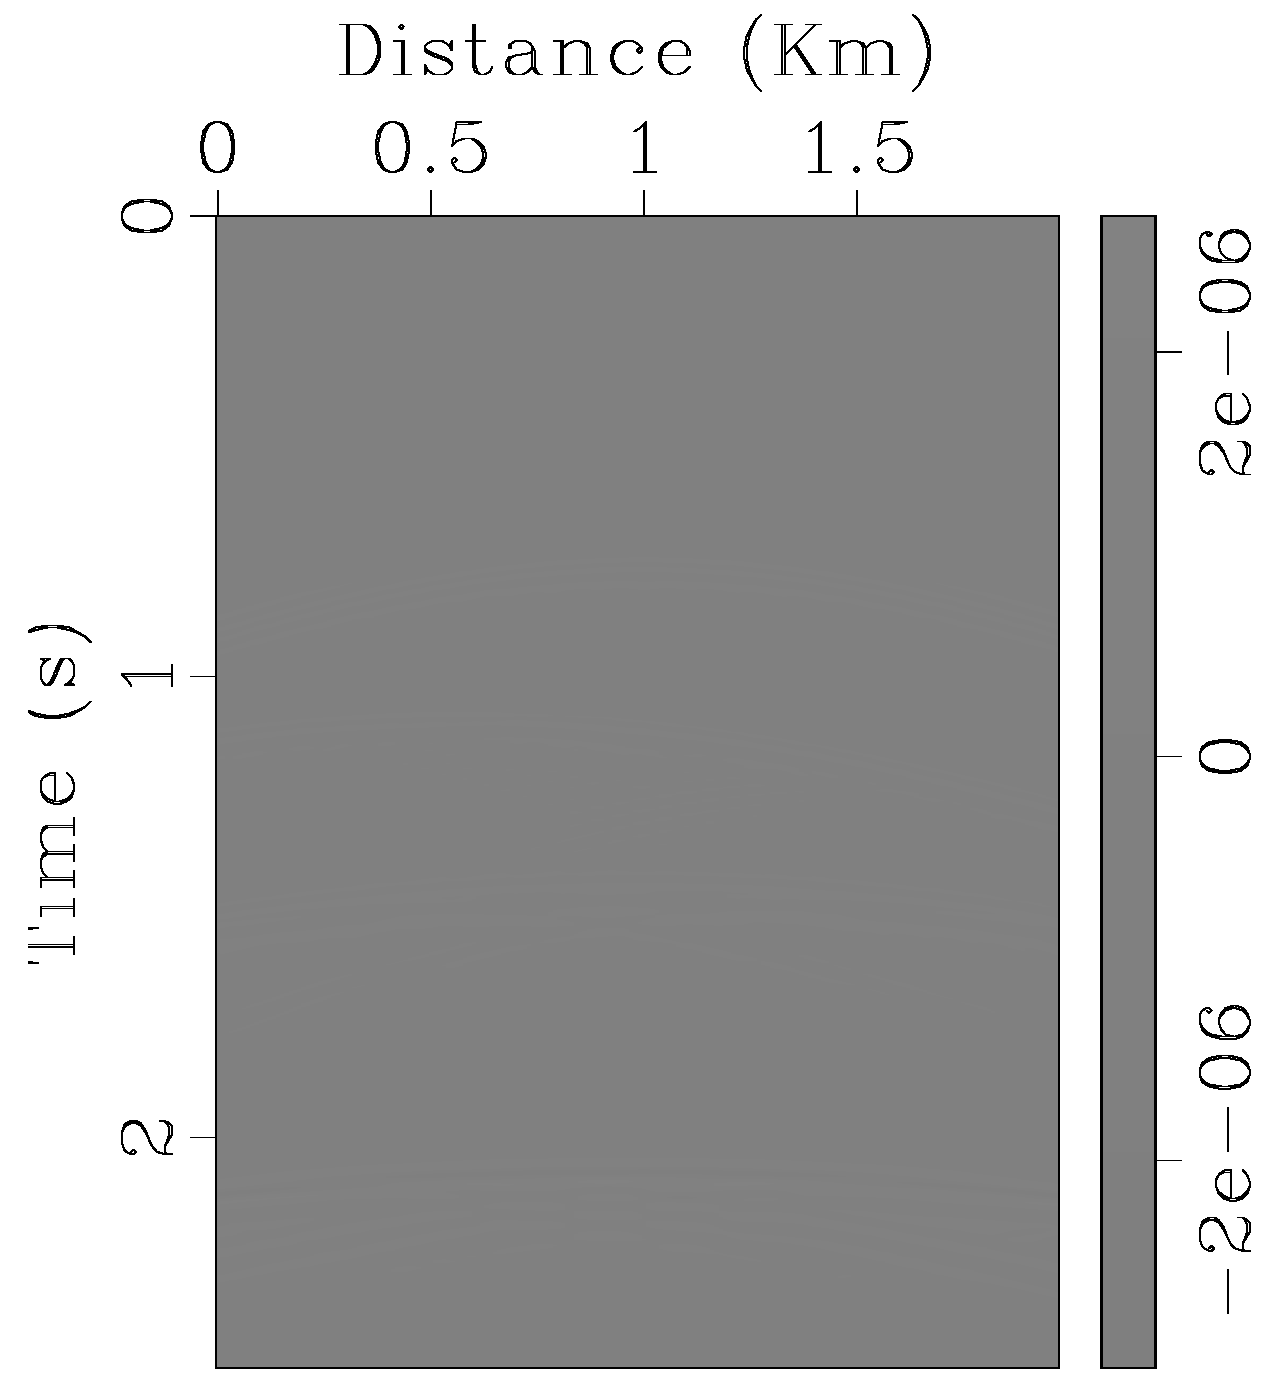
\includegraphics[width=0.47\linewidth]{figure/diff30}}
	\fcaption{数据残差比较:(a)在1km处的单炮记录;(b)跟初始模型正演数据的残差;
	(c)迭代30次后的数据残差。}{(a) The observed data for the shot
	at 1km, (b) the residual with the initial $Q$, and (c) the residual with the 
	$Q$-RWI inverted $Q$.}[数据残差对比结果]
    \label{fig:record_diff}
\end{figure*}

\begin{figure*}[!htbp]
    \centering
	\subfigure[]{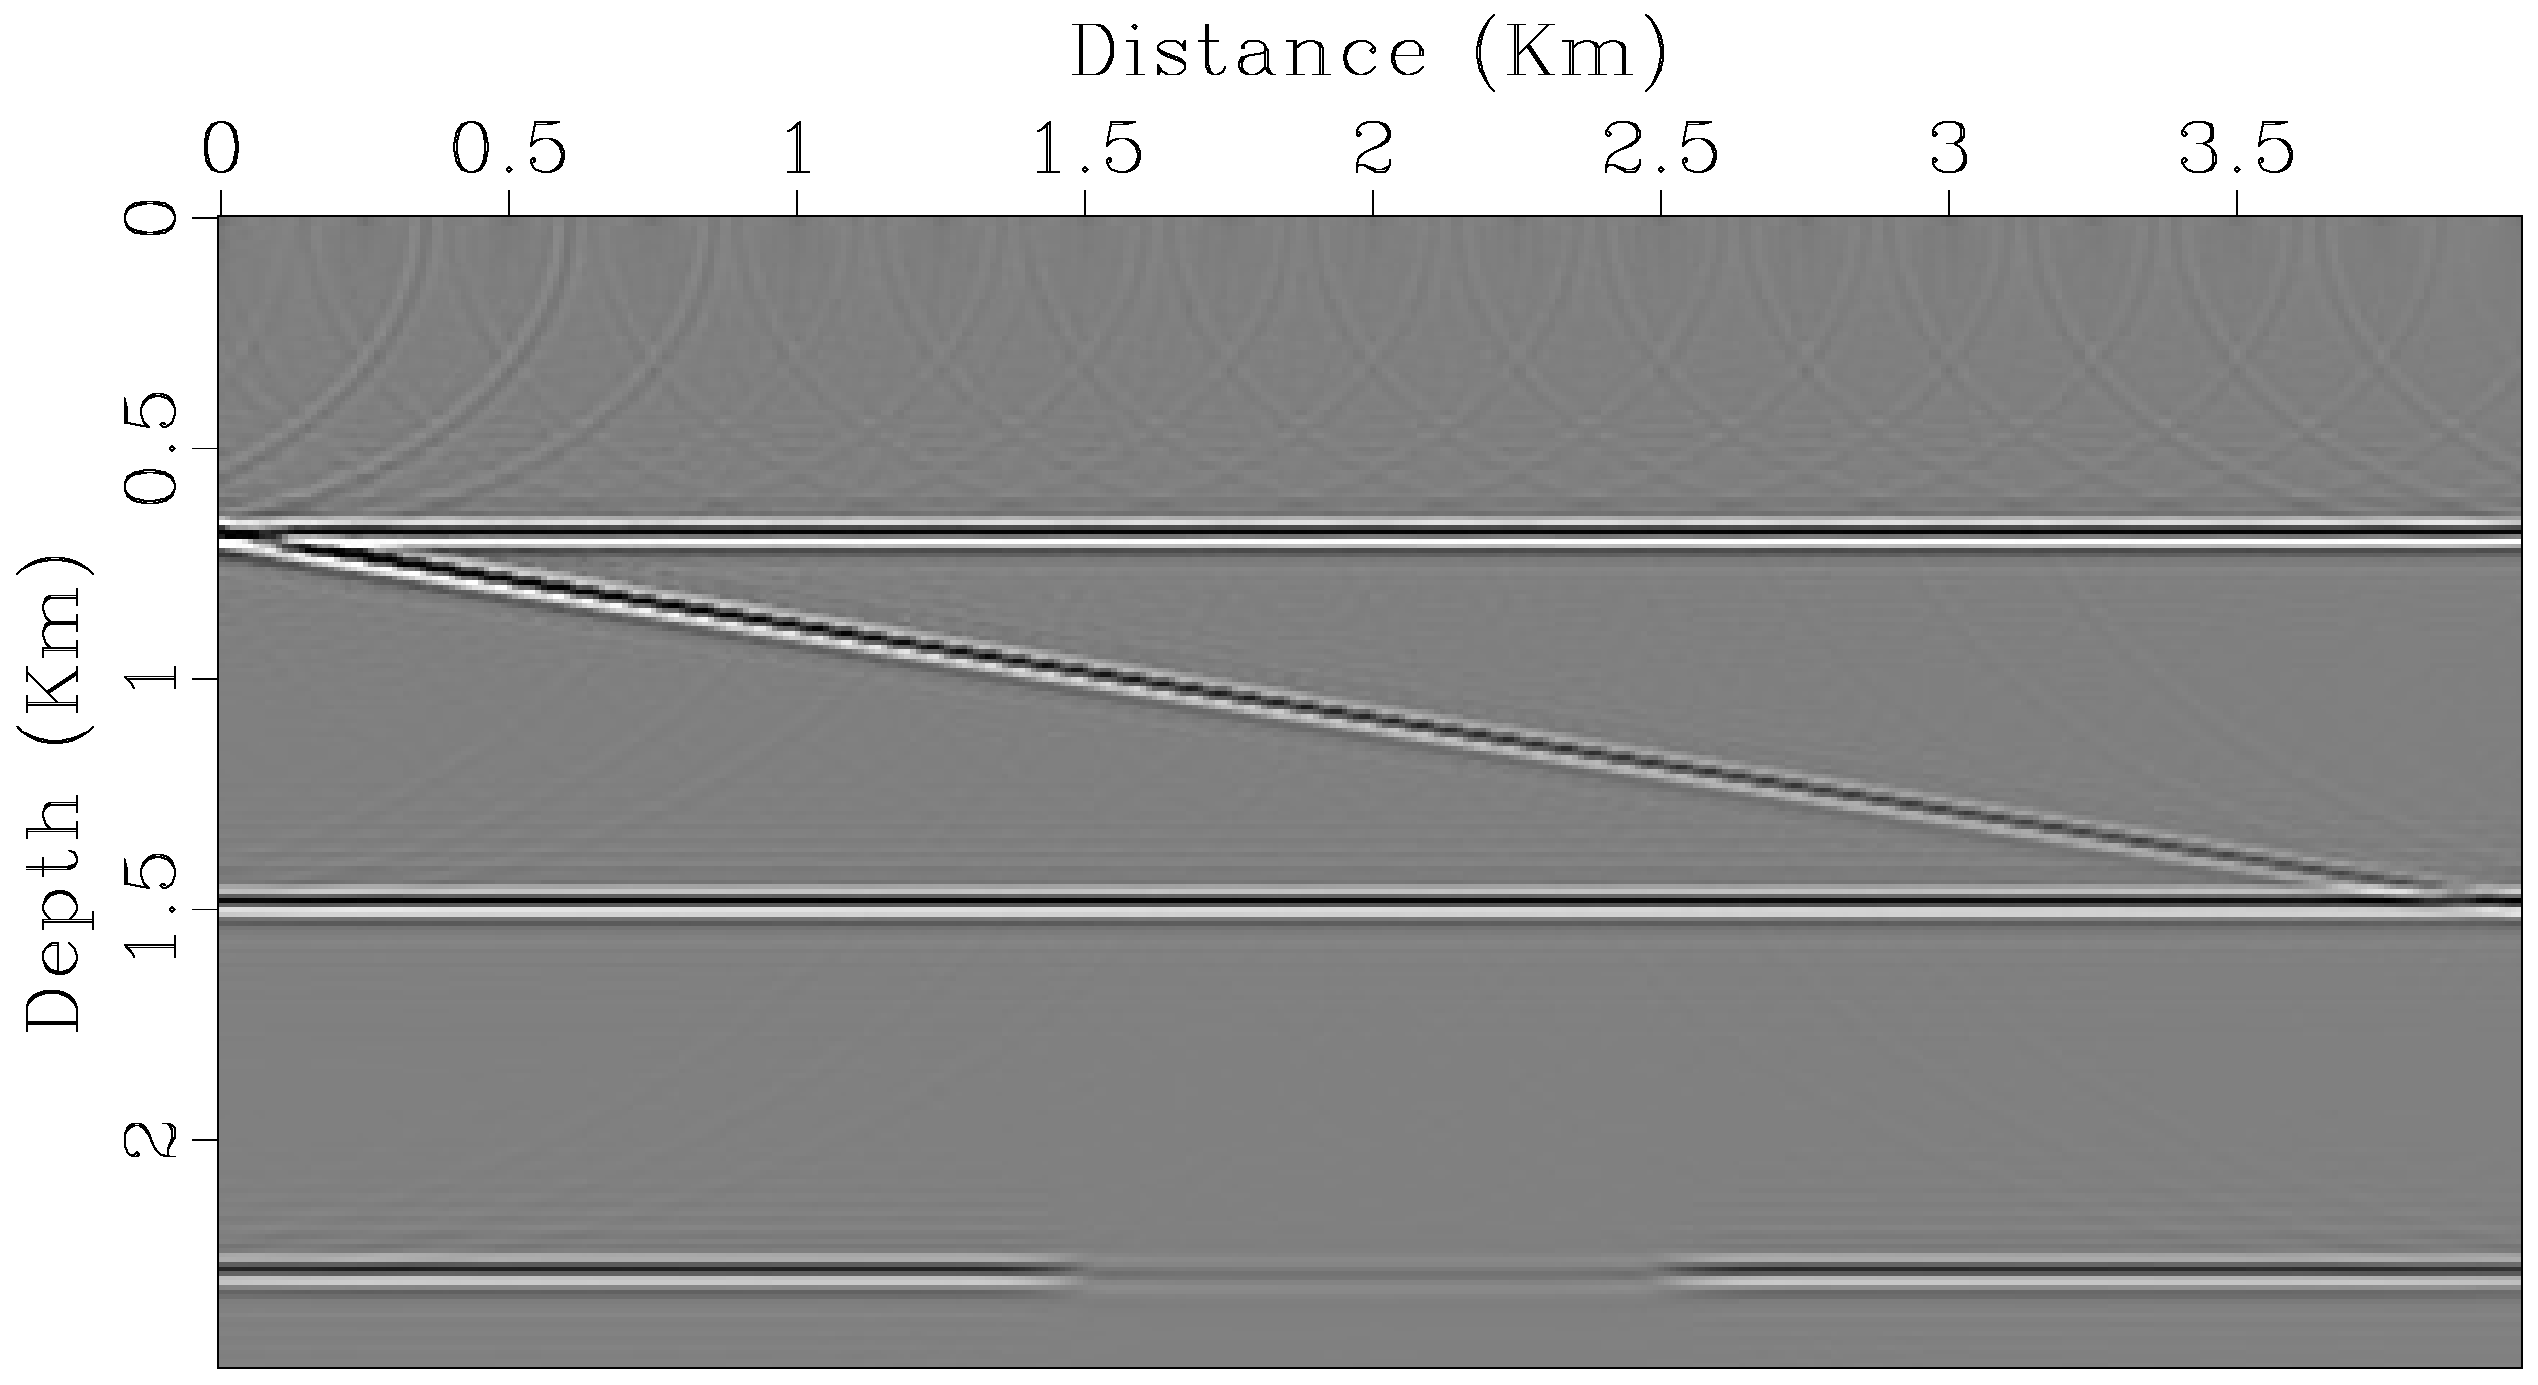
\includegraphics[width=0.72\linewidth]{figure/rtm_no400x250}}
	\subfigure[]{\includegraphics[width=0.72\linewidth]{figure/rtm_true400x250}}
	\subfigure[]{\includegraphics[width=0.72\linewidth]{figure/rtm_fq400x250}}
	\fcaption{$Q$-RTM成像结果:(a)初始$Q$补偿结果;(b)真实$Q$补偿结果;
	$Q$-RWI反演$Q$补偿结果。}{$Q$-compensated RTM images using initial
	$Q$ model (a); true $Q$ model (b) and $Q$-RWI inverted $Q$ model (c).}
	[$Q$-RTM成像结果]
    \label{fig:rtm_model}
\end{figure*}


%%==================================================
%% conclusion.tex for SJTU Master Thesis
%% based on CASthesis
%% modified by wei.jianwen@gmail.com
%% version: 0.3a
%% Encoding: UTF-8
%% last update: Dec 5th, 2010
%%==================================================

\chapter*{结论与展望\markboth{结论与展望}{}}
\addcontentsline{toc}{chapter}{结论与展望}

\newcommand{\backsection}[1]{\vskip 2.8ex
	\begin{flushleft}
		{\zihao{-3}\textbf{#1}}
	\end{flushleft}
	\vskip 0.8ex}


\backsection{结论}

地下介质普遍存在非弹性衰减,它对地震波传播、成像、弹性参数反演以及储层预测均有强烈
影响。本文第二章较系统地总结了地震衰减的数学物理描述,并比较了两类常用粘声
波方程的特性以及在成像、反演中的应用。
吸收衰减对地震波传播的宏观影响是一种沿波路径的累加效应。为了重构地下介质中深部
的衰减模型,本文利用反射波数据来增加波路径的照明深度,首次将$Q$反演纳入
RWI框架。在速度准确的情况下,$Q$-RWI能很好地恢复地下中深部宏观衰减模型。论文最后
通过引入峰值频率移动目标函数来降低$Q$-RWI对高波数速度模型的依赖性。通过论文
的研究,主要得到了以下几点认识:

(1)在勘探地震频段,SLS粘声波方程和常$Q$模型粘声方程均能很好描述地震波在衰减地层中的能量损失
和速度频散效应。在进行成像和反演时,既要进行能量补偿同时也必需要保证速度频散关系不变。
常$Q$模型对应的一些近似波动方程可以将能量损失项和速度频散项分开,在进行一次偏移成像时,
用其构造的反传方程能在补偿能量的同时保持速度频散关系不变。而SLS粘声波方程通过记忆变量
来控制能量损失和速度频散,很难用其构造将能量补偿和速度频散分开的反传方程。
两类方程的伴随方程虽对能量进行了二次衰减,但保持了原有的速度频散关系。在进行
迭代反演(如$Q$-LSRTM)时,这两类方程有相同的效果,因为多次迭代能补偿损失的能量。
在进行$Q$反演时,两类方程均可用,但要注意在进行反传时必需用其对应的伴随方程以保证物理关系
的正确性。

(2)在低波数和高波速速度成分均已知的情况下,$Q$-RWI利用反射波数据对中深部
模型进行照明,可以很好恢复中深部宏观$Q$模型。因为反射数据对浅层覆盖不足,$Q$-RWI
对浅层模型的分辨率不高且存在多解性,其浅层反演结果是一种等效模型。这种等效结果虽不能
满足储层预测需求,但足以满足中深层反射波数据$Q$-RTM的需要。

(3)地震数据的峰值频率属性主要与地震本征衰减有关。通过引入峰值频率移动目标函数,很大
程度降低了$Q$-RWI对高波数速度的依赖性。峰值频率对高波数速度的大小和极性不敏感,但
依赖于高波速模型的相对几何结构,即要保证Born正演中的高波数模型不能改变子波的形状。数值实验
证明用层状速度平滑差的结构作为Born正演中伪扰动模型是可行的。
在实际勘探中,常规处理流程可获取光滑背景速度,再通过偏移成像获得地下反射界面位置,
然后将统一伪扰动结构赋在反射界面处,就可以用作反射数据峰值频率模拟计算所需的高波数速度模型。

\backsection{创新点}

本论文的主要创新点有:

(1)首次将$Q$反演纳入RWI框架,用粘声波动方程作为引擎计算反射波路径以适应复杂地层
情况,通过反射波路径恢复中深部的衰减模型,其反演结果满足$Q$-RTM与$Q$-LSRTM
的需求。

(2)通过将最小化峰值频率移动作为目标函数,降低了$Q$-RWI对高波数速度的依赖性。
通过用层状速度平滑差的结构作为Born正演中的高波数扰动模型,使$Q$-RWI更加符合实际需要。

\backsection{不足与展望}

$Q$-RWI反演仍然存在很多尚待深入研究的问题。作者认为今后还应在以下几方面
继续研究:

(1)当背景速度不准确时,偏移再反偏移的数据与原始数据存在差异,此时$Q$-RWI由于数据匹配不准而
产生误差。如何克服背景速度误差的影响值得研究。

(2)本文是在顺序反演的框架下进行研究的,即先反演速度再反演$Q$值。在实际反演中,地震衰减的存在
也影响速度反演的精度,如何联合反演背景速度和$Q$模型也是非常有意义的研究课题。

(3)本文未进行实际地震数据测试。在实际数据中噪音、薄层调谐、子波形状如何影响峰值频率也是一个值得
研究的点。

(4)此外,除了地层本征衰减,强烈的介质非均匀性造成的散射也可能引起地震波振幅衰减与相位畸变。
因此,在实际应用中,有必要分析散射衰减是不是可以忽略。




\appendix	% 使用英文字母对附录编号,重新定义附录中的公式、图图表编号样式
\renewcommand\theequation{\Alph{chapter}--\arabic{equation}}	
\renewcommand\thefigure{\Alph{chapter}--\arabic{figure}}
\renewcommand\thetable{\Alph{chapter}--\arabic{table}}

\chapter{低秩近似求解DCQ方程}
\citeB{zhu.harris:2014}推导的DCQ方程有如下的频散关系:
\begin{equation}
    \frac{\omega^2}{c^2}=-\eta|\mathbf{k}|^{2\gamma+2}-i\omega\tau|\mathbf{k}|^{2\gamma+1},
	\label{eq:disp}
\end{equation}
求解方程(\ref{eq:disp})的$\omega$有,
\begin{equation}
	\omega=\frac{-ip_1+p_2}{2},
\end{equation}
其中
\begin{equation}
	p_1=\tau c^2|\mathbf{k}|^{2\gamma+1},
\end{equation}
\begin{equation}
	p_2=\sqrt{-\tau^2c^4|\mathbf{k}|^{4\gamma+2}-4\eta c^2|\mathbf{k}|^{2\gamma+2}}.
\end{equation}
在时间域决定波传播的相移函数可以定义为:
\begin{equation}
	\phi_1(\mathbf{x},\mathbf{k},\Delta t)=\mathbf{k}\cdot\mathbf{x}+\frac{-ip_1+p_2}{2}\Delta t,
	\label{eq:phase_func}
\end{equation}

在$Q$-RTM中,通过改变方程(\ref{eq:disp})右端第二项的符号来补偿振幅衰减,而频散控制项的符号
必须保持不变。因此,衰减补偿常$Q$方程对应的频散关系为:
\begin{equation}
    \frac{\omega^2}{c^2}=-\eta|\mathbf{k}|^{2\gamma+2}+i\omega\tau|\mathbf{k}|^{2\gamma+1},
	\label{eq:disp1}
\end{equation}
其对应的复共轭相位函数为:
\begin{equation}
	\phi_2(\mathbf{x},\mathbf{k},\Delta t)=\bar{\phi_1}(\mathbf{x},\mathbf{k},\Delta t)
    =\mathbf{k}\cdot\mathbf{x}+\frac{ip_1+p_2}{2}\Delta t,
	\label{eq:phase_func1}
\end{equation}
相位函数$\phi_1$和$\phi_2$都包含波数的分数阶指数,同时是空间位置$\mathbf{x}$和波数$\mathbf{k}$
的函数。\citeB{sun.zhu:2015}用这种相位函数来延拓粘声波场,并允许分数阶指数$\gamma(\mathbf{x})$
随空间变化。单步混合域算子可以整合成如下的Fourier积分算子:
\begin{equation}
	p(\mathbf{x},t+\Delta t)=\int \hat{p}(\mathbf{k},t)e^{i\phi(\mathbf{x},\mathbf{k},\Delta t)}
	d\mathbf{k},
	\label{eq:one_step}
\end{equation}
其中$\hat{p}$是$p$的空间Fourier变换。方程(\ref{eq:one_step})的伴随形式为:
\begin{equation}
	\hat{p}(\mathbf{k},t)=\int p(\mathbf{x},t+\Delta t)e^{-i\bar{\phi}(\mathbf{x},\mathbf{k},
	\Delta t)}d\mathbf{k},
\end{equation}
式中$\bar{\phi}$是$\phi$的共轭。
将方程(\ref{eq:phase_func})带入方程(\ref{eq:one_step})中可以显示得到粘声方程的正传算子
\begin{equation}
	\begin{aligned}
		p(\mathbf{x},t+\Delta t)&=\int \hat{p}(\mathbf{k},t)e^{i\phi_1(\mathbf{x},
		\mathbf{k},\Delta t)}d\mathbf{k}, \\
		&=\int \hat{p}(\mathbf{k},t)e^{i\mathbf{k}\cdot\mathbf{x}+(p_1+ip_2)\Delta t/2}d\mathbf{k}.
	\end{aligned}
	\label{eq:forward}
\end{equation}
其对应的伴随算子为:
\begin{equation}
	\begin{aligned}
		\hat{p}_{adj}(\mathbf{k},t)&=\int p(\mathbf{x},t+\Delta t)e^{-i\bar{\phi}_1(\mathbf{x},
		\mathbf{k},\Delta t)}d\mathbf{k}, \\
		&=\int \hat{p}(\mathbf{x},t+\Delta t)e^{-i\mathbf{k}\cdot\mathbf{x}+(p_1-ip_2)\Delta t/2}d\mathbf{k}.
	\end{aligned}
	\label{eq:adjoint}
\end{equation}
伴随算子(\ref{eq:adjoint})作为反传算子补偿了$Q$-RTM中的速度频散,但是会二次衰减波场的能量,所以不适合
$Q$-RTM。
在$Q$-RTM中,正传和反传波场都应该补偿能量的衰减,其对应的正传和反传算子如下:
\begin{equation}
	\begin{aligned}
		p_{comp}(\mathbf{x},t+\Delta t)&=\int \hat{p}(\mathbf{k},t)e^{i\phi_2(\mathbf{x},
		\mathbf{k},\Delta t)}d\mathbf{k}, \\
		&=\int \hat{p}(\mathbf{k},t)e^{i\mathbf{k}\cdot\mathbf{x}+(-p_1+ip_2)\Delta t/2}d\mathbf{k},
	\end{aligned}
	\label{eq:forward1}
\end{equation}
和
\begin{equation}
	\begin{aligned}
		\hat{p}_{comp-adj}(\mathbf{k},t)&=\int p(\mathbf{x},t+\Delta t)e^{-i\bar{\phi}_2(\mathbf{x},
		\mathbf{k},\Delta t)}d\mathbf{k}, \\
		&=\int \hat{p}(\mathbf{x},t+\Delta t)e^{-i\mathbf{k}\cdot\mathbf{x}+(-p_1-ip_2)\Delta t/2}d\mathbf{k}.
	\end{aligned}
	\label{eq:adjoint1}
\end{equation}

以上方程中的混合域算子$e^{i\phi(\mathbf{x},\mathbf{k},\Delta t)}$统一
用$W(\mathbf{x},\mathbf{k})$来表示,由于
其涉及空间-波数域的相互变换,导致数值计算非常昂贵。\citeB{fomel.ying:2013}用低秩近似来降低
混合域算子的计算量。其形式可以表示为如下形式:
\begin{equation}
	W(\mathbf{x},\mathbf{k})\approx\sum_{m=1}^M\sum_{n=1}^NW(\mathbf{x},\mathbf{k}_m)a_{mn}
	W(\mathbf{x}_n,\mathbf{k})
\end{equation}
因此$p(\mathbf{x},t+\Delta t)$的计算有如下的形式:
\begin{equation} 
	p(\mathbf{x},t+\Delta t)\approx\sum_{m=1}^MW(\mathbf{x},\mathbf{k}_m)\(\sum_{n=1}^Na_{mn}\(\int
	e^{i\mathbf{x}\mathbf{k}}W(\mathbf{x}_n,\mathbf{k})p(\mathbf{k},t)d\mathbf{k}\)\).
	\label{eq:lowrank}
\end{equation}
方程(\ref{eq:lowrank})的计算量相当于每个时间步做$N$次反Fourier变换,在实际中,$N<10$。


\chapter{DCQ方程反射全波形反演梯度推导}





\backmatter	% 文后无编号部分 

%% 参考资料

\bibliography{bib/preference}


%% 致谢、发表论文、参与项目、简历
%%==================================================
%% thanks.tex for SJTU Master Thesis
%% based on CASthesis
%% modified by wei.jianwen@gmail.com
%% version: 0.3a
%% Encoding: UTF-8
%% last update: Dec 5th, 2010
%%==================================================

\begin{thanks}
	
\zihao{4}\hangju{1}
时光荏苒,一晃七年已过。同济见证了一名懵懂少年变成合格硕士的全部历程,
我也见证了同济七年的辉煌。本硕七载青春,留在心里的是道不尽的感激,我
仍将怀着感激之情在母校的怀抱里攻读博士学位以谢母校的哺育之恩。

在这里我首先要感谢我的导师程玖兵教授。从大四至今已四年有余,我的每一
点进步都与您的悉心指导有关。您不仅传授我专业知识,还在生活中给予我巨大
的帮助。从概念到理论,从编程到撰文,您在科研中的每一处细节都用精益求精的
态度来要求自己和我们。每一次的讨论都让我茅塞顿开,每一次的谈话都让我
备受鼓舞。不仅如此,您从不懈怠的工作态度,助人为乐的崇高品格都在
潜移默化的影响着我。如今硕士论文已将完成,其中每一页里面都包含了您的心血
与付出。恩师之情,不轻于父母,无以为报。很荣幸能继续聆听您的教诲,
我将更加努力向您学习。

地震组大家庭是我梦想起航的地方,在这里付出了艰辛与努力,收获了知识、技能
与成长。在这里特别感谢董良国教授这几年来的关心与指导,最初是您的提点让我走上
了科研的道路。同时也感谢耿建华教授在储层地球物理课以及组会上的悉心指导,感谢
王华忠教授在成像与反演以及信号处理中的耐心研讨,感谢宋海滨教授填补的地震海洋学
方面的知识空缺,感谢杨锴教授在地震数据处理
课中的细心讲解,感谢钟广法和刘堂晏教授在地震解释、测井以及岩石物理方面的尽心
辅导,感谢刘玉柱教授在层析成像中的指点迷津,感谢赵峦啸、屠宁和王本锋老师在
组会讨论中的指点和帮助。再次由衷感谢各位老师的传道育人,让我们这些学子受益终身。

同门之谊令我终生难忘。特别感谢王腾飞、王晨龙两位博士师兄对我学习和计算机编程上的
耐心指导以及出差时的细心照顾。感谢已毕业的四位硕士师兄滕龙、康玮、段鹏飞、杨涛
以及尚颖霞师姐留下的丰厚研究成果,让我收益良多。感谢同组的杨亚丽、阮晟、徐文才、
刘学义、于洋、阮轮、熊一能在生活和学业上的无私帮助。此外,感谢一众博士师兄姐王雄文、
李晓波、王义、王毓伟、黄超、迟本鑫、杨积忠、于鹏飞、孙敏傲、张博、杨靖康,你们在
科研上的讨论使我少走了许多弯路。感谢何文俊、王毕文、刘伟刚、康昊的手足之情以及
同届同学三年的同窗之情。

最后,我要感谢父母的养育之恩、弟弟的手足之情,感谢所有亲朋好友在我读书期间
的支持。我特别感谢女朋友饶竹红女士,九年同窗、七年陪伴之情。此生有幸,在最美
的年华遇见你,夫复何求,良辰美景,愿此生与你共度。


\end{thanks}
 	%% 致谢
%%==================================================
%% pub.tex for SJTU Master Thesis
%% based on CASthesis
%% modified by wei.jianwen@gmail.com
%% version: 0.3a
%% Encoding: UTF-8
%% last update: Dec 5th, 2010
%%==================================================

\begin{publications}{99}

\item \textbf{P. Zou} and J.B. Cheng, Pseudo-spectral method using rotated 
	staggered grid for elastic wave propagation in 3D arbitrary anisotropic 
	media. \textit{Geophysical Prospecting}, 2018, 66, 47-61. \hspace{3ex}(SCI)

\vspace{-2ex}
\item J.B. Cheng, T. Alkhalifah, Z.D. Wu, \textbf{P. Zou} and C.L. Wang, 
	Simulating propagation of decoupled elastic waves using low-rank 
	approximate mixed-domain integral operators for anisotropic media.
	\textit{Geophysics}, 2016, 81(2), T63--T77. \hspace{3ex}(SCI)

\vspace{-2ex}
\item \textbf{P. Zou} and J.B. Cheng, Modified pseudo-spectral method for wave 
	propagation in arbitrary anisotropic media. \textit{78th EAGE 
	Conference \& Exhibition 2015}, Vienna, Austria. \hspace{3ex}(EI)

\vspace{-2ex} 
\item \textbf{P. Zou} and J.B. Cheng, Modified pseudo-spectral method for wave 
	propagation in general anisotropic media. \textit{SPG/SEG Beijing 
	2016 International Geophysical Conference}, Beijing, China.
    
\end{publications}


	%% 发表论文
%%==================================================
%% projects.tex for SJTU Master Thesis
%% based on CASthesis
%% modified by wei.jianwen@gmail.com
%% version: 0.3a
%% Encoding: UTF-8
%% last update: Dec 5th, 2010
%%==================================================

\begin{projects}{99}
%
    \item 各向异性弹性波模式分离与矢量分解及其全波成像应用,国家自然科学基金项目
		(\textit{NO. 41474099})
	\item 各向异性弹性波模式分离与矢量分解理论方法研究,上海市自然科学基金项目
		(\textit{NO.14ZR1442900})
	\item Full waveform inversion of seismic data for reservior attributes, the Competitive
		Research Grants Program funded by the University Research Fund of King Abdullah University
		of Science and Technology (KAUST), Saudi Arabia (\textit{Award 2230}).     
\end{projects}
  %% 参与的项目

\end{document}
